\chapter{Elektromagnetische Wellen}\label{emwellen}
 \section{Grundlagen} \label{emwellgrdl}
 \subsection{Felder}
 Es wird vom vollen Satz der Maxwell-Gleichungen ausgegangen ($\nearrow$\ref{ind},\ref{quellf},\ref{durchf},\ref{gauss}). Das Medium sei \textbf{linear, homogen, isotrop} ($\nearrow$\ref{matlinhomis}). Die Maxwell-Gleichungen können entkoppelt werden, wünschenswert sind Gleichungen in denen nur elektrische oder nur magnetische Feldgrößen vorkommen:
		        \begin{align}
			        \underbrace{\rot \rot }_{\nearrow \text{\ref{rotrot}} }\vec{E}                 & = -\frac{\partial }{\partial t}\rot \vec{B}  = -\frac{\partial}{\partial t}\left(\mu \vec{J}+\mu \varepsilon\frac{\partial \vec{E}}{\partial t}\right) \nonumber \\
			        \grad \div \vec{E}-\Delta \vec{E}                                    & = -\mu \frac{\partial \vec{J}}{\partial t}-\mu\varepsilon\frac{\partial^2 \vec{E}}{\partial t^2}                                                  \nonumber     \\
			        \grad \frac{\rho_\text{V}}{\varepsilon}-\Delta \vec{E}               & = -\mu \frac{\partial \vec{J}}{\partial t}-\mu \varepsilon\frac{\partial^2 \vec{E}}{\partial t^2}                                                    \nonumber  \\
			        \Aboxed{\Delta \vec{E}-\varepsilon\mu \frac{\partial^2\vec{E}}{\partial t^2} & = \grad \frac{\rho_\text{V}}{\varepsilon}+\mu \frac{\partial \vec{J}}{\partial t}} \label{Hentk}
		        \end{align}
		   Analog für $\vec{H} $:
		        \begin{align}
			        \rot \rot \vec{H}                                      & = \rot \vec{J} +\varepsilon\frac{\partial}{\partial t}\rot \vec{E} = \rot \vec{J}-\varepsilon\mu\frac{\partial^2}{\partial t^2}\vec{H}                     \nonumber   \\
			        \grad \underbrace{\div \vec{H} }_{=0} - \Delta \vec{H} & = \rot \vec{J}-\varepsilon\mu\frac{\partial^2}{\partial t^2}\vec{H} \nonumber \\
			        \Aboxed{ \Delta \vec{H} -\varepsilon\mu\frac{\partial^2}{\partial t^2}\vec{H} &= -\rot \vec{J}} \label{Eentk}
		        \end{align}
Auf der linken Seite wird jeweils der selbe Operator auf die Felder angewandt. Es handelt sich um \textbf{Wellengleichungen}.
\subsection{Potentiale}
		   Durch die Definition des \textbf{Skalarpotentials}  \(\phi\) ($\nearrow$\ref{potsdef}) und des \textbf{Vektorpotentials} \( \vec{A}\) ($\nearrow$\ref{potadef}) werden die homogenen Maxwell-Gleichungen automatisch erfüllt ($\nearrow$\ref{auterf1},\ref{auterf2}). Das Einsetzen der Potentialdefinitionen in die inhomogenen Maxwell-Gleichungen ($\nearrow$\ref{durchf}\ref{gauss}) ergibt \ref{bestphi} und \ref{besta}.
		   Unter Nutzung der \textbf{Lorenz-Eichung} ($\nearrow$\ref{lorenzbdg}) vereinfachen sich die Bestimmungsgleichungen wesentlich zu \ref{bestskalarpotlor} und \ref{bestvekpotlor}. Damit sind die partiellen Differentialgleichungen für die Potentiale \textbf{entkoppelt}. Mit der \textbf{Strahlungseichung} (Coulomb-Eichung, $\nearrow$\ref{coulbdg}) folgt ähnliches unter Beachtung von \ref{bestvekcoul}, wenn die Lösung nur in weiter Entfernung zu Ladungen interessiert (also \( \phi = 0 \) im Lösungsgebiet angenommen werden kann):
		        \begin{equation}
			        \boxed{\Delta  \vec{A}-\varepsilon\mu\frac{\partial^2 \vec{A}}{\partial t^2}=-\mu \vec{J}}
		        \end{equation}
 \section{Homogene Wellengleichung}
	  Es wird von den entkoppelten Gleichungen für die Felder ($\nearrow$\ref{Eentk},\ref{Hentk}) und für die Potentiale in \textbf{Lorenzeichung} ($\nearrow$\ref{bestskalarpotlor},\ref{bestvekpotlor}; homogen, linear, isotrop $\leftrightarrow$Vakuum:$\mu\leftrightarrow\mu_0,\varepsilon\leftrightarrow\varepsilon_0$) ausgegangen. Unter den \textbf{Annahmen} 
	  \begin{equation}\label{annhomwell}
	  \text{hli, }\quad\rho_\text{V}=0 \quad \text{ und }\quad\vec{J}=\vec{0},
	  \end{equation}
	   also keine Quellen im Lösungsgebiet, besteht immer die gleiche formale Struktur:
		        \begin{equation}\label{homwell}
			       \boxed{ (\Delta -\varepsilon\mu\frac{\partial^2}{\partial t^2})\Psi = \square\Psi = 0    }
		        \end{equation}
		        Dabei wird der \textbf{Wellenoperator} $\square$ (auch D'Alembert-Operator oder Quabla-Operator) definiert:
		        \begin{equation}
		        	\boxed{\square = \Delta - \varepsilon\mu\frac{\partial^2}{\partial t^2}}
		        \end{equation}
		        Gleichungen dieses Typs heißen Wellengleichungen. \(\Psi = \Psi(\vec{r} , t)\) steht für eine Komponente von \(\vec{E}\), \(\vec{B} \), \(\vec{D} \), \(\vec{H} \), \( \vec{A}\) oder \(\phi\), sofern die Potentiale in Lorenz-Eichung sind. Im Vakuum gilt \ref{vaklicht} (wobei $\mu_0$ seit 2019 ein experimenteller Wert mit geringem relativen Fehler zu $4\pi \dots$ ist). Ansonsten gilt
		        \begin{equation}\label{geschwepsmu}
		        \boxed{	\varepsilon\mu = \frac{1}{ v_\mathrm{c}^2}}
		        \end{equation}
		       Dabei ist \( v_\mathrm{c}\) die Lichtgeschwindigkeit im Medium. Es gilt:
		        \begin{equation}
			        c\ge  v_\mathrm{c} = \frac{1}{\sqrt{\varepsilon\mu}} = \frac{1}{\sqrt{\varepsilon_0\mu_0}\sqrt{\varepsilon_\mathrm{r}\mu_\mathrm{r}}} = \frac{c}{\sqrt{\varepsilon_\mathrm{r}\mu_\mathrm{r}}} =\frac{c}{n}     
		        \end{equation}
		        Dabei definiert man den \textbf{Brechungsindex}:
		        \begin{equation}
		        	\boxed{n = \sqrt{\varepsilon_\mathrm{r}\mu_\mathrm{r}}}
		        \end{equation} 
  \section{Ebene Wellen als Lösung der homogenen Wellengleichung}\label{ebwell}
  \subsection{Allgemeine ebene Wellen}
	   Im Folgenden soll die \textbf{Homogene Wellengleichung} ($\nearrow$\ref{homwell},\ref{geschwepsmu}) betrachtet werden:
		        \begin{equation}\label{homwell1}
			        \Delta \Psi (\vec{r} , t) - \frac{1}{ v_\mathrm{c}^2}\frac{\partial ^2}{\partial t^2}\Psi (\vec{r} , t) = 0 \qquad\quad \square \Psi (\vec{r} , t) = 0
		        \end{equation}
	Für diese Gleichung sollen Lösungen gefunden werden. Zunächst beschränkt sich die Betrachtung auf Lösungen, die sich nur in \textbf{einer Richtung ausbreiten} und daher \textbf{Ebene Wellen} genannt werden. Der \textbf{Ansatz} zur Lösung dieser Gleichung ist, dass $\Psi$ auf spezielle Weise von $\vec{r}$ und $t$ abhängt:
		        \begin{equation}\label{anseben}
			        \boxed{\Psi(\vec{r} , t) = \Psi (\omega t + \vec{k}\cdot\vec{r} )  = \Psi  (\omega t + k_x x+ k_y y + k_z z )}
		        \end{equation}
	Dabei wird  die \textbf{Phasenfunktion} definiert:
	\begin{equation}
		\varphi (\vec{r} , t) = \omega t + \vec{k}\cdot\vec{r}
	\end{equation}
		$\vec{k}$ wird \textbf{Wellenvektor} genannt und dessen Betrag $k$ \textbf{Wellenzahl}. Mit dem Ansatz kann man zunächst $\Delta \Psi$ und $ \frac{\partial^2}{\partial t^2}\Psi$ bilden:
		        \begin{equation*}\begin{split}
				         \Delta \Psi&= \frac{\partial^2 \Psi}{\partial x^2} + \frac{\partial^2 \Psi}{\partial y^2} + \frac{\partial^2 \Psi}{\partial z^2}=\frac{\partial}{\partial \varphi}\left(\frac{\partial \Psi}{\partial\varphi}\frac{\partial \varphi}{\partial x}\right)\frac{\partial \varphi}{\partial x} + \frac{\partial}{\partial \varphi}\left(\frac{\partial \Psi}{\partial\varphi}\frac{\partial \varphi}{\partial y}\right)\frac{\partial \varphi}{\partial y} + \frac{\partial}{\partial \varphi}\left(\frac{\partial \Psi}{\partial\varphi}\frac{\partial \varphi}{\partial z}\right)\frac{\partial \varphi}{\partial z} \\
				         &=  (k_x^2+k_y^2+k_z^2)\cdot\frac{\partial^2 \Psi}{\partial \varphi^2} =k^2\cdot\frac{\partial^2 \Psi}{\partial \varphi^2}  \\
				            \frac{\partial^2}{\partial t^2}\Psi &= \frac{\partial}{\partial \varphi}\left(\frac{\partial \Psi}{\partial\varphi}\frac{\partial \varphi}{\partial t}\right)\frac{\partial \varphi}{\partial t}\\
				            &=\omega^2\frac{\partial^2 \Psi}{\partial \varphi^2}\\
		\end{split}\end{equation*}
	Das kann man dann in \ref{homwell1} einsetzen:
		\begin{equation}\begin{split}
				         &0 = \left(  k^2 -\frac{\omega^2}{  v_\mathrm{c}^2}\right)\frac{\partial^2 \Psi}{\partial \varphi^2}\\
				         \Rightarrow &\vec{k}\cdot\vec{k}= \left(-\vec{k}\right)\cdot \left(-\vec{k}\right) =  k^2  \quad \quad \text{ mit }\quad \quad k:=|\pm\vec{k}|\\
				         \Rightarrow & \boxed{k= \frac{\omega}{v_\mathrm{c}}=\omega \sqrt{\mu\varepsilon} }
			        \end{split}\end{equation}
		      Den gerahmten Zusammenhang nennt man auch lineare \textbf{Dispersionsrelation}. Ohne Beschränkung der Allgemeinheit kann dabei $\omega\geq 0$ angenommen werden (wegen $\pm$). Für jeden Wert des Parameters \(\omega\) (\textbf{Kreisfrequenz}) gibt es zwei mögliche Werte für den \textbf{Wellenvektor} $\pm \vec{k}$ mit der gleichen Wellenzahl \textbf{Wellenzahl} \( k = |\pm\vec{k}|\). Die allgemeine Lösung (zum gewählten Ansatz) der homogenen Wellengleichung ist somit:
		        \begin{equation}\label{algebwell}\begin{split}
			        \Aboxed{ \Psi (\vec{r} , t) &= \sum_\omega \left( \Psi_+ (\omega t + \vec{k}\cdot\vec{r} ) + \Psi_- (\omega t - \vec{k}\cdot\vec{r} ) \right) }     \\ \vec{k} &=  k \frac{\vec{k}}{ k} = \frac{\omega}{ v_\mathrm{c}}\frac{\vec{k}}{ k} =\frac{\omega}{ v_\mathrm{c}} \vu{ k}
		       \end{split} \end{equation}
		  Da die $\omega$ i.A. überabzählbar sind, wäre statt dem Summenzeichen ein Integralzeichen exakter. Ist die \textbf{Phasenfunktion} \(\varphi_\pm (\vec{r} , t) = \omega t \pm \vec{k}\cdot\vec{r}  \) konstant, also \( \varphi (\vec{r} , t) = \const \), folgt daraus \( \Psi = \text{const}\). Betrachtet wird der Zeitpunkt \(t=t_0\):
		        \begin{equation}
			        \varphi_\pm (\vec{r} , t_0) = \omega t_0 \pm \vec{k}\cdot\vec{r}  \to \varphi_\pm=\const \Leftrightarrow  \vec{k}\cdot\vec{r} =\const
		        \end{equation}
		   Durch $\vec{k}\cdot\vec{r}=\const$ wird eine Ebene senkrecht zu $\vec{k}$ beschrieben:
	  \begin{center}
		  \resizebox{.5\textwidth}{!}{\input{res/ebeneWelle}}
	  \end{center}
	 Orte, die zu einem Zeitpunkt \(t=t_0\) gleiche Werte \(\varphi\) haben, liegen auf Ebenen senkrecht zu \(\vec{k}\).  Diese Orte nennt man \textbf{Wellenfront}. Hängt $\Psi$ bspw. periodisch von $\varphi$ ab, werden durch $\Psi=\const$ mehrere Ebenen beschrieben. Betrachtet man ein \(t_1 > t_0\) mit gleichem Wert für $\varphi=\varphi_0$, hat man Orte wiederkehrender Phase:
	   \begin{center}
	 	\resizebox{.5\textwidth}{!}{\input{res/ebeneWelle2}}
	 \end{center}
		        \begin{equation}\begin{split}
				        \varphi_0 &= \omega t_0 + \vec{k}\cdot\vec{r} _0 \stackrel{!}{=} \omega t_1 \pm \vec{k}\cdot\vec{r} _1\\
				        \Rightarrow \pm \vec{k}\cdot\vec{r} _1 &= \varphi_0 - \omega t_1  \\   \vec{k}\cdot\vec{r} _1 &= k r_{1\parallel}\quad \text{ mit } \quad r_{1\parallel}=\frac{\vec{k}\cdot\vec{r} _1}{ k}  \\
				        \Rightarrow \pm r_{1\parallel} &=\frac{\varphi_0}{ k} - \frac{\omega}{k} t_1\\
				        \Rightarrow r_{1\parallel} &= \pm\frac{\varphi_0}{ k} \mp \frac{\omega}{k} t_1\\
			        \end{split}\end{equation}
		  $r_{1\parallel} $ ist eine lineare Funktion der Zeit. Im Fall \(\omega t {+} \vec{k}\cdot\vec{r} \) bewegt sich die Wellenfront (also die Orte wiederkehrender Phase) in Richtung \(-\vec{k}\), im Fall \(\omega t {-} \vec{k}\cdot\vec{r} \) in Richtung $+\vec{k}$. Außerdem wird die
		   \textbf{Phasengeschwindigkeit} definiert, also die Geschwindigkeit, mit der sich  eine konstante Phase des Schwingungsterms (bspw. 0) ausbreitet. Mit dem Ansatz \(\omega t {-} \vec{k}\cdot\vec{r} =0\) folgt:
		   \begin{equation}
		   	\boxed{ v_\mathrm{p} =\frac{\dd r_{\parallel}}{\dd t} }\stackrel{\text{hier}}{=} \frac{\omega}{ k} \stackrel{\text{hier}}{=}{ v_\mathrm{c}}
		   \end{equation}
	Es ist zu beachten, dass die Phasengeschwindigkeit nicht immer gleich der Lichtgeschwindigkeit im jeweiligen Medium ist. 
 \subsection{Harmonische ebene Wellen}\label{harmebwell}
  		 \textbf{Ebene Wellen} sind Lösungen der homogenen Wellengleichung Gleichung, für die allgemein \ref{algebwell} gilt. Hier soll nur die \textbf{hinlaufende} Lösung für \textbf{einen} Wert von \(\omega\) betrachtet werden, also:
		        \begin{equation}
			        \Psi(\vec{r} , t) = \Psi(\varphi_-(\vec{r} , t)) = \Psi(\omega t - \vec{k}\cdot\vec{r} )
		        \end{equation}
		   Außerdem soll eine spezielle Phasenfunktion \(\varphi\) gewählt werden, sodass \(\Psi\) einer Funktion mit \textbf{harmonischer Zeitabhängigkeit} entspricht:
		        \begin{equation}\begin{split}
			        \Aboxed{\underline{\Psi}(\vec{r} , t) &= \underline{\Psi}_0  \mathrm{e}^{\mathrm{j}(\omega t -\vec{k} \cdot \vec{r} )} }  \\ \Psi(\vec{r} , t) &= \re{\underline{\Psi}(\vec{r} , t)}
		        \end{split}\end{equation}
	     Beachte, dass hier im Gegensatz zu \ref{phasoren} die Zeitabhängigkeit mit in $\underline{\Psi}$ hinein definiert wird. Es wird also nur noch der Realteil gebildet und auf die Normierung auf $\mathrm{e}^{\mathrm{j}\omega t}$ verzichtet ($\nearrow$\ref{ansig}).
  \subsubsection{Wellenlänge und Frequenz}
	 	 Zu einem \textbf{festen Zeitpunkt} haben Flächen gleicher Werte einen festen Abstand $\Delta r_\Vert$. Die Bedingung dafür, dass die Flächen den gleichen Wert haben ist bei harmonischer Zeitabhängigkeit:
	 	 \begin{equation}
	 	 	\Delta\vec{r} \cdot\vec{k} = \Delta r_\Vert \cdot  k  = 2\pi n \quad \quad n\in\IZ  
	 	 \end{equation}
	 	 Für den Fall $n=1$ wird $\Delta r_\Vert$ als \textbf{Wellenlänge} $\lambda$ definiert:
	 	 \begin{equation}
	 	 	\Delta r_\Vert \cdot  k  = 2\pi                           \quad\implies\quad \boxed{\Delta r_\Vert = \frac{2\pi}{ k} =\lambda}
	 	 \end{equation}
	 	 Damit folgt:
 		        \begin{equation}
			      k = \frac{2\pi}{\lambda}   = \frac{\omega}{ v_{\mathrm{p}}} \quad \implies \quad \boxed{ v_{\mathrm{p}}=\frac{\omega}{2\pi}\cdot \lambda}  =  v_\mathrm{c} \underset{\substack{\varepsilon = \varepsilon_0 \\ \mu = \mu_0}}{=} c
		        \end{equation}
		  An einem \textbf{festen Ort} wiederholen sich gleiche Werte nach einer festen Zeit $\Delta t$. Die Bedingung dafür, dass $\Psi$ den gleichen Wert hat ist bei harmonischer Zeitabhängigkeit:
		  \begin{equation}
		  	 \Delta t \omega     = 2\pi  n     \quad \quad n\in \IZ                              
		  \end{equation}
		  Für den Fall $n=1$ wird $\Delta t$ als \textbf{Periodendauer} $T$ definiert. Außerdem führt man die \textbf{Kreisfrequenz} $\omega$ und die \textbf{Frequenz} $f$ ein: 
		  \begin{equation}
		  	\Delta t \omega = 2\pi \quad\implies\quad \boxed{\Delta t = T  = \frac{2\pi}{\omega} = \frac{1}{f}}
		  \end{equation}
		  Damit gilt:
		        \begin{equation}
			     \boxed{ v_{\mathrm{p}}= f \cdot \lambda}  =  v_\mathrm{c}\underset{\substack{\varepsilon = \varepsilon_0                                            \\ \mu = \mu_0}}{=} c
		        \end{equation}
  \subsubsection{$E-$ und $B-$Feld: TEM-Wellen}\label{tem}
	Zunächst wird angenommen, dass \(\vec{E}\) und \(\vec{B} \) unterschiedliche Kreisfrequenzen und Wellenvektoren haben könnten:
		        \begin{align}\label{ebharm}
			        \ubar{\vec{E}} & = \ubar{\vec{E}}_0  \mathrm{e}^{\mathrm{j}(\omega t - \vec{k}\cdot\vec{r} )} & \vec{\ubar{B}} & = \vec{\ubar{B}}_0  \mathrm{e}^{\mathrm{j}(\omega ' t - \vec{k} \ensuremath{'}\cdot\vec{r} )}
		        \end{align}
		  Einerseits gilt das Induktionsgesetz \ref{ind}:
		        \begin{equation}\begin{split}
				        \rot \ubar{\vec{E}} = -\frac{\partial \vec{\ubar{B}}}{\partial t}= -\mathrm{j}\omega ' \vec{\ubar{B}}
		\end{split}\end{equation}  
	Andererseits lässt sich mit $\ubar{\vec{E}} = \ubar{\vec{E}}_0  \mathrm{e}^{\mathrm{j}(\omega t - \vec{k}\cdot\vec{r} )}$ analytisch ein Ausdruck für $ \rot \ubar{\vec{E}} $ berechnen. Die Rechnung erfolgt beispielsweise in kartesischen Koordinaten. Wenn das Ergebnis dann wieder koordinatenfrei geschrieben werden kann, hat man eine in allen Koordinatensystemen gültige Aussage gefunden. Dieses Prinzip kann man häufig anwenden. Hier resultiert:
\begin{equation}\begin{split} 
				        \rot \ubar{\vec{E}}& = -\mathrm{j}\left( \vec{k} \times \ubar{\vec{E}}\right)\\
				        \Rightarrow  -\mathrm{j}\left( \vec{k} \times \ubar{\vec{E}}_0 \right)  \mathrm{e}^{\mathrm{j}\left(\omega t - \vec{k}\cdot\vec{r} \right)}  &\stackrel{!}{=} -\mathrm{j}\omega' \vec{\ubar{B}}_0  \mathrm{e}^{\mathrm{j}\left(\omega' t -\vec{k}'\cdot\vec{r} \right)}
			        \end{split}\end{equation}
		 Dieser Ausdruck muss für alle \(t\) und alle \(\vec{r} \) gelten. Damit folgt:
		        \begin{equation}\begin{split}
				         \left. \begin{array}{l}
					        \omega = \omega', \quad    \vec{k} = \vec{k}' \\
					        \vec{k}\times\ubar{\vec{E}}_0 = \omega\vec{\ubar{B}}_0
				        \end{array}
				        \right\rbrace \vec{\ubar{B}}_0 = \frac{1}{\omega} \vec{k} \times\ubar{\vec{E}}_0 \quad\implies \quad \boxed{\vec{\ubar{B}} = \frac{1}{\omega} \vec{k} \times\ubar{\vec{E}}}\\
			        \end{split}\end{equation}
		  Es folgt also, dass \( \ubar{\vec{E}}\) und \(\vec{\ubar{B}}\) \textbf{in Phase} sind und \(\vec{\ubar{B}}\) senkrecht auf der von \(\vec{k}\) und \(\ubar{\vec{E}}\) aufgespannten Ebene steht:
		        \begin{equation}
			       \boxed{ \vec{\ubar{B}}_0 \Vert \left(\vec{k} \times \ubar{\vec{E}}_0 \right)}
		        \end{equation}
 	Nun wird mit \ref{gauss} (Annahme: \(\rho_\text{V} = 0\)) und \ref{quellf} weiter gerechnet. $E$ und $B$ haben dabei die Form aus \ref{ebharm}, durch formale Divergenzbildung folgt:
		        \begin{align}
			        \div \vec{E} & = 0 & \Rightarrow \quad -\vec{k}\cdot \ubar{\vec{E}}_0 & = 0 & \curvearrowright &  & \boxed{\vec{k}\bot \ubar{\vec{E}}_0} \\
			        \div \vec{B} & = 0 & \Rightarrow \quad -\vec{k}\cdot \vec{\ubar{B}}_0 & = 0 & \curvearrowright &  & \boxed{\vec{k}\bot \vec{\ubar{B}}_0}
		        \end{align}
	Mit \ref{durchf} (Annahme: \(\vec{J}=\vec{0}\)) folgt durch formale Rotationsbildung:
		        \begin{align}
			        \rot \vec{\ubar{B}} &= \frac{1}{ v_{\mathrm{p}}^2}\frac{\partial \ubar{\vec{E}}}{\partial t} \nonumber\\
			         -\mathrm{j}\vec{k}\times\vec{\ubar{B}}_0 &= \mathrm{j}\omega\frac{1}{ v_{\mathrm{p}}^2}\ubar{\vec{E}}_0 \nonumber\\
			          \ubar{\vec{E}}_0 &= -\frac{ v_{\mathrm{p}}^2}{\omega}\vec{k} \times \vec{\ubar{B}}_0 \nonumber\\
			                                                                                                                                                                                                               & \Rightarrow  \boxed{\ubar{\vec{E}}_0 \| \left(\vec{\ubar{B}}_0 \times \vec{k} \right)}
		        \end{align}
 \begin{minipage}{.7\textwidth}
 	 \(\vec{E}\), \(\vec{B} \) und \(\vec{k}\) bilden ein \textbf{orthogonales Rechtssystem}. Sowohl $E$ als auch $B$ sind transversal zur Ausbreitungsrichtung. Man spricht von \textbf{Transversalen Elektromagnetischen Wellen (TEM-Wellen)}, weil $E$ und $B$ keine Komponente longitudinal zur Ausbreitungsrichtung haben. 
 \end{minipage}
 \begin{minipage}{.29\textwidth}
 	\raggedleft
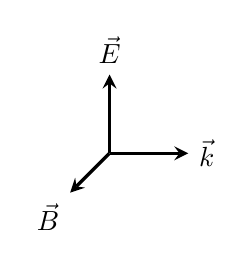
\begin{tikzpicture}[line width = 1.2pt, line join=round,x={(.5cm,.5cm)},y={(1cm, 0cm)},z={(0cm,1cm)},>=stealth]
	% x-Richtung
	\draw [->] (0,0,0) -- (-1,0,0) node[anchor=north east] {$\vec{B}$};
	% y-Richtung
	\draw [->] (0,0,0) -- (0,1,0) node[anchor=west] {$\vec{k}$};
	% z-Richtung
	\draw [->] (0,0,0) -- (0,0,1) node[anchor=south] {$\vec{E}$};
\end{tikzpicture}
 \end{minipage}\\
 Es ist anzumerken, dass $E$ und $B$ nur in sehr vielen Spezialfällen senkrecht zueinander sind. Da $H$ und $E$ bei ebenen Wellen über den Feldwellenwiderstand zusammenhängen, ist es schwierig durch Superposition ebener Wellen einen nicht senkrechten Fall zu konstruieren (beide Wellen müssen im gleichen Medium das gleiche $H/E$-Verhältnis haben). Dennoch gilt, dass die Rotation eines Vektors ist nicht immer senkrecht zum Vektor selber ist, das Kreuzprodukt mit dem Nabla-Operator wirkt also nicht wie ein \enquote{normales} Kreuzprdukt. Das Induktionsgesetz ($\nearrow$\ref{ind}) ist demnach bspw. kein Grund, warum $E$ und $B$ stets senkrecht sein sollten.
 \subsubsection{Zusammenfassung der Formeln für harmonische Ebene Wellen}
 Zusammenfassend gelten für harmonische ebene Wellen die folgenden Formeln:
 \begin{equation}\label{ebwellzsfg}\begin{split}
 		\ubar{\vec{E}}(\vec{r} , t) & =\ubar{\vec{E}}_0 \mathrm{e}^{\mathrm{j}(\omega t - \vec{k}\cdot\vec{r} )} \\
 		\vec{\ubar{B}}(\vec{r} , t)  &=\vec{\ubar{B}}_0 \mathrm{e}^{\mathrm{j}(\omega t - \vec{k}\cdot\vec{r} )}  \\
 		 \vec{\ubar{B}}_0 &= \frac{1}{\omega} \left(\vec{k} \times \ubar{\vec{E}}_0\right)= \frac{ k}{\omega} \left(\vu{k} \times \ubar{\vec{E}}\right) = \frac{1}{ v_\mathrm{p}} \left(\vu{k} \times \ubar{\vec{E}}\right) = \sqrt{\varepsilon\mu} \left(\vu{k} \times \ubar{\vec{E}}\right) \\
 		 |\vec{\ubar{B}}_0|^2 &= \frac{1}{ v_\mathrm{c}^2} |\ubar{\vec{E}}_0|^2 \\
 		v_\mathrm{c} &= \frac{1}{\sqrt{\varepsilon\mu}} = \frac{\omega}{ k} = v_\mathrm{p}\\
 			\vec{\ubar{H}} &= \frac{1}{\mu}\vec{\ubar{B}} = \frac{1}{\mu}\sqrt{\varepsilon\mu} \left(\vu{k} \times \ubar{\vec{E}}\right) = \sqrt{\frac{\varepsilon}{\mu}} \left(\vu{k} \times \ubar{\vec{E}}\right) = \frac{1}{Z} \left(\vu{k} \times \ubar{\vec{E}}\right)\\
	\ubar{\vec{E}} &= -Z \left(\vu{k} \times \vec{\ubar{H}}\right)
 \end{split}\end{equation}
Neu wurde hierbei noch die \textbf{Feldwellenimpedanz} (auch Feldwellenwiderstand) eingeführt:
\begin{equation}\label{feldwellenwid}
	\boxed{Z=\sqrt{\frac{\varepsilon}{\mu}}}
\end{equation}
  \subsubsection{Beispiel}        
     Es wird \(\vec{k} =  k \cdot \vu{z}\) gesetzt. Damit folgt:
      \begin{equation*}\begin{split}
         \ubar{\vec{E}}&=\left( \ubar{E}_{0x} \vu{x} + \ubar{E}_{0y}\vu{y}\right)  \mathrm{e}^{\mathrm{j}(\omega t - k z)}  ;\quad \ubar{E}_{0x}, \ubar{E}_{0y} \in \IC\\
        \vec{\ubar{B}} &= \left( \ubar{B}_{0x} \vu{x} + \ubar{B}_{0y}\vu{y}\right) \mathrm{e}^{\mathrm{j}(\omega t -  k z)}  ;\quad \ubar{B}_{0x}, \ubar{B}_{0y} \in \IC
       \end{split}\end{equation*}
	Außerdem gilt ($\ubar{E}_{0x}=\left|\ubar{E}_{0x}\right|\mathrm{e}^{\mathrm{j}\varphi_x}$):
		        \begin{equation*}\begin{split}
		        \vec{E}&=\re{\vec{\ubar{E}}}=\left|\ubar{E}_{0x}\right|\vu{x}\cos (\omega t - kz +\varphi_x)+\left|\ubar{E}_{0y}\right|\vu{y}\cos (\omega t - kz +\varphi_y)\\
			      \vec{B} &= \frac{1}{\omega}\vec{k}\times \vec{E} =  \frac{1}{ v_{\mathrm{p}}}\vu{k}\times\vec{E} = \frac{1}{ v_{\mathrm{p}}}\vu{z}\times\vec{E}       
		        \end{split}\end{equation*}
		 Das kann man visualisieren (hier $E\parallel \vu{x}$):
	  \begin{center}
		  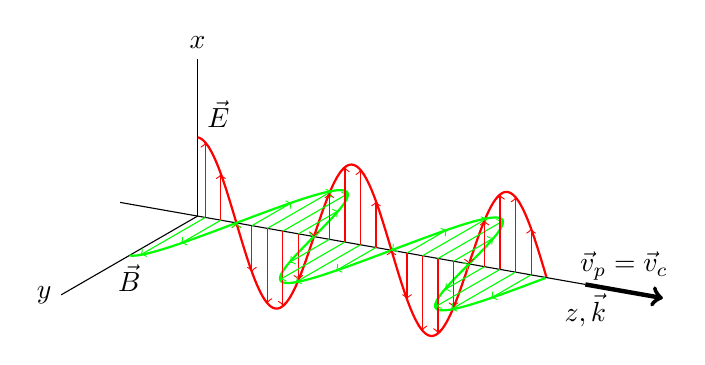
\begin{tikzpicture}[x={(-10:1cm)},y={(90:1cm)},z={(210:1cm)}]
	% Axes
	\draw (-1,0,0) -- (5,0,0) node[below] {$z, \vec{k}$};
	\draw (0,0,0) -- (0,2,0) node[above] {$x$};
	\draw (0,0,0) -- (0,0,2) node[left] {$y$};
	% Propagation
	\draw[->,ultra thick] (5,0,0) -- node[above] {$\vec{v}_p=\vec{v}_c$} (6,0,0);
	% Waves
	\draw[red,thick] plot[domain=0:4.5,samples=200] (\x,{cos(deg(pi*\x))},0);
	\draw[green,thick] plot[domain=0:4.5,samples=200] (\x,0,{cos(deg(pi*\x))});
	% Arrows
	\foreach \x in {0.1,0.3,...,4.4} {
			\draw[->,red] (\x,0,0) -- (\x,{cos(deg(pi*\x))},0);
			\draw[->,green] (\x,0,0) -- (\x,0,{cos(deg(pi*\x))});
		}
	% Labels
	\node[above right] at (0,1,0) {$\vec{E}$};
	\node[below] at (0,0,1) {$\vec{B}$};
\end{tikzpicture}
		  \begin{minipage}{.5\linewidth}
			  \[
				  v_\mathrm{p} = \frac{\omega}{k} = \frac{|\vec{E}|}{|\vec{B}|} \stackrel{\text{hier}}{=} v_\mathrm{c}
			  \]
			  \begin{tabular}{r@{${}={}$}p{.8\linewidth}}
				  $E$   & Amplitude des elektrischen Feldes                                            \\
				  $B$   & Amplitude der Magnetflussdichte                                              \\
				  $v_\mathrm{p}$ & Phasengeschwindigkeit                                                        \\
				  $v_\mathrm{c}$ & Lichtgeschwindigkeit im Medium                                               \\
				  $c$   & \raggedright   Vakuum Lichtgeschwindigkeit $= 299792458\mathrm{\frac{m}{s}}$
			  \end{tabular}
		  \end{minipage}%
		  \begin{minipage}{.5\linewidth}
			  \[
				  v_\mathrm{c} = \frac{1}{\sqrt{\mu \varepsilon}} =\frac{c}{\sqrt{\mu_r \varepsilon_r}} = \frac{c}{n}
			  \]
			  \begin{tabular}{r@{${}={}$}p{.8\linewidth}}
				  $\mu_0$         & magnetische Permitivität des Vakuums $= 4\pi\cdot 10^{-7}\mathrm{\frac{H}{m}}$ \\
				  $\varepsilon_0$ & \raggedright  elektrische Permeabilität des Vakuums $= \frac{1}{\mu_0 c^2}$
			  \end{tabular}
		  \end{minipage}
	  \end{center}
 \subsection{Polarisation ebener Wellen}\label{poleb}
		 Es werden \textbf{monochromatische ebene Wellen} (eine Frequenz), die in \(+z\)-Richtung propagieren betrachtet:
		        \begin{align}\label{polallglsg}
			        \ubar{\vec{E}} & = \left( \ubar{E}_{0x}\vu{x} + \ubar{E}_{0y}\vu{y}\right) \mathrm{e}^{\mathrm{j}( \omega t -  k z)}                         &
			        \vec{\ubar{B}} & = \frac{1}{ v_{\mathrm{p}}}\left(-\ubar{E}_{0y}\vu{x} +\ubar{E}_{0x}\vu{y}\right)  \mathrm{e}^{\mathrm{j}(\omega t -  k z)} & v_{\mathrm{p}}= \frac{\omega}{k} \stackrel{\text{hier}}{=}  v_{\mathrm{c}}
		        \end{align}
		  Dabei sind:
		        \begin{equation}\begin{split}
				        \ubar{E}_{0x} &= \vert \ubar{E}_{0x} \vert \cdot  \mathrm{e}^{\mathrm{j}\varphi_x} \text{ - komplexe Komponente in \(x\)-Richtung bei \(t=0, z=0\)}\\
				        \ubar{E}_{0y} &= \vert \ubar{E}_{0y} \vert \cdot  \mathrm{e}^{\mathrm{j}(\varphi_x+ \delta)} \text{ - analog für \(y\)-Komponente}\\
				        \vec{E} (\vec{r} , t) &= \re{\ubar{E}(\vec{r} , t)} = E_x \vu{x} + E_y \vu{y} \text{ - Physikalische Lösung}\\
				        E_x &= \vert \ubar{E}_{0x} \vert \cos(\omega t -  k z + \varphi_x )\\
				        E_y &= \vert \ubar{E}_{0y} \vert \cos(\omega t -  k z + \varphi_x +\delta)\\
				        \varphi_x &: \text{ - gemeinsamer Phasenwinkel \(\to\) relativ unwichtig}\\
				        \delta &: \text{ - relative Phase \(\to\) \textbf{Fallunterscheidung}}
			        \end{split}\end{equation}
		 Anhand der relativen Phase wird unterschieden:
		        \begin{enumerate}
			        \item \(\delta = 0, \pm \pi , \pm 2\pi, \ldots\)
			        \item \(  \delta = \pm \frac{\pi}{2}, \pm \frac{3\pi}{2},\ldots \quad ;\quad\vert \ubar{E}_{0x} \vert = \vert \ubar{E}_{0y} \vert = \hat{E} \)
			        \item \( \delta = \pm \frac{\pi}{2}, \pm \frac{3\pi}{2},\ldots \quad ;\quad\vert \ubar{E}_{0x} \vert \neq \vert \ubar{E}_{0y} \vert \)
			        \item \(\delta\) und \(\vert \ubar{E}_{0x} \vert, \vert \ubar{E}_{0y} \vert\) beliebig
		        \end{enumerate}
		        Die Fälle werden im Folgenden diskutiert.
  \subsubsection{1. Fall: Lineare Polarisation}
		  Es wird \(\delta = z \cdot \pi ,\quad z \in \IZ\quad\rightarrow\quad \delta = \textcolor{green!70}{0}, \textcolor{red}{\pm \pi} , \textcolor{green!70}{\pm 2\pi}, \ldots\) betrachtet. Für den Cosinus gilt die Beziehung:
		        \begin{equation}\begin{split}
				        \begin{split}
					        \cos ( \alpha + \delta ) = \pm \cos \alpha \quad;\quad &\textcolor{green!70}{+} :   0,\pm 2\pi, \pm 4\pi, \ldots\\
					        & \textcolor{red}{-} :   \pm \pi, \pm 3\pi, \ldots
				        \end{split}
			        \end{split}\end{equation}
		   Hiermit ergibt sich für das elektrische Feld:
		        \begin{equation}\begin{split}
				        \Rightarrow \vec{E}&= \underbrace{(\vert \ubar{E}_{0x} \vert \vu{x} \pm \vert \ubar{E}_{0y}\vert \vu{y})}_{\substack{\text{fester Vektor, orts- und}\\ \text{zeitunabhängig}}} \cos (\omega t -  k z + \varphi_x)\\
				        &= \hat{E}\cdot \vu{E}\cos (\omega t -  k z + \varphi_x )\\
				        \hat{E} &= \vert \vec{E} \vert = \sqrt{\vert \ubar{E}_{0x} \vert ^2 + \vert \ubar{E}_{0y} \vert ^2}
			        \end{split}\end{equation}
		  Weil $E$ immer in der selben Richtung $\vu{E}$ schwingt, spricht man von linearer Polarisation. Der \textbf{Polarisationswinkel} ist folgendermaßen definiert:
	  \begin{center}
		  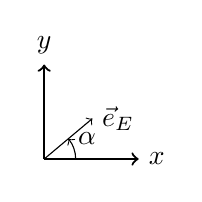
\begin{tikzpicture}[scale=0.4]
	% Achsen zeichnen
	\draw[->,thick] (0,0) -- (3,0) node[right] {$x$};
	\draw[->,thick] (0,0) -- (0,3) node[above] {$y$};
	%Plot
	\draw[->] (0,0) --(40:2) node[right] {$\vec{e}_E$};
	\draw[->] (0:1)arc(0:40:1) node[right] {$\alpha$};
\end{tikzpicture}
		  \raisebox{.75cm}{\(\Rightarrow\tan \alpha = \pm \dfrac{|\ubar{E}_{0y}|}{|\ubar{E}_{0x}|}\) }
	  \end{center}
	  Die allgemeine Lösung ($\nearrow$ \ref{polallglsg})ist eine Überlagerung zweier linear polarisierter Beiträge in \(x\)- bzw. \(y\)-Richtung. \textbf{Somit ist jede beliebige Polarisation darstellbar als Überlagerung zweier zueinander senkrechter linearer Polarisationen.} Somit müssen nur zwei Fälle unterschieden werden um jede beliebige Polarisation zu diskutieren. Sendet man beispielsweise ein linear polarisiertes Signal aus, dann kann es passieren, dass eine Komponente (Zerlegung in $x$- und $y$-Komponente) aufgrund von Inhomogenitäten auf dem Weg stärker gedämpft wird. So kann sich die Polarisation drehen. Das ist insbesondere bei der Dimensionierung von Antennen zu beachten.
  \subsubsection{2. Fall: Zirkulare Polarisation}
		  Nun wird \(\delta = (2m+1) \frac{\pi}{2}, \quad m \in \mathbb{Z} , \quad\delta = \pm \frac{\pi}{2}, \pm \frac{3\pi}{2},\ldots \quad ;\quad\vert E_{0x} \vert = \vert E_{0y} \vert = \hat{E} \) betrachtet. Für den Cosinus gilt die Beziehung:
		        \begin{equation}\begin{split}
				        \begin{split}
					        \cos ( \alpha + \delta ) = \mp \sin \alpha \quad;\quad &\textcolor{red}{+} :   -\frac{\pi}{2} + m (2\pi) \quad\textcolor{green!70}{-} :    +\frac{\pi}{2} + m (2 \pi), \quad m \in \IZ
				        \end{split}
			        \end{split}\end{equation}
		  Hiermit ergibt sich für das elektrische Feld:
		        \begin{equation}\begin{split}
				        \vec{E} &= \hat{E}(\cos(\omega t -  k z + \varphi_x)\vu{x} \mp \sin (\omega t -  k z + \varphi_x)\vu{y})
			        \end{split}\end{equation}
		  Für ein festes \(z\) oder \(t\) ist das ein Kreis mit Radius \(\hat{E}\). Deshalb spricht man von \textbf{zirkularer Polarisation}. Zur Unterscheidung rechts vs. links schaut man an einem festen Ort in $\vec{k}$-Richtung und beobachtet, wie sich der Zeiger dreht. In der folgenden Grafik ist $\vec{k}$ aus der Ebene hinaus definiert, entsprechend muss man aus der Ebene hinausschauen.
		        \begin{center}
			        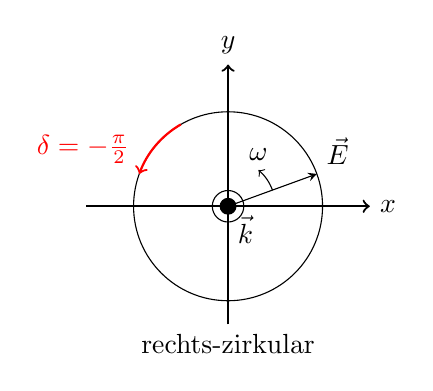
\begin{tikzpicture}[]
	% Achsen zeichnen
	\draw[->,thick] (-1.8,0) -- (1.8,0) node[right] {$x$};
	\draw[->,thick] (0,-1.5) -- (0,1.8) node[above] {$y$};
	%Plot
	%\draw[style=dashed] (-1.27,-1.05) rectangle (1.27,1.05);
	\draw (0, 0) circle (1.2);
	\draw (0, 0) circle (.2);
	\draw[fill=black] (0, 0) circle (.1);
	\draw (0,0) node[below right] {$\vec{k}$};
	\draw[->,>=stealth] (0,0)--(20:1.2) node[above right] {$\vec{E}$};
	\draw[->] (20:.6) arc (20:50:.6) node [above] {$\omega$};
	\draw [->,thick,color=red] (120:1.2) arc (120:160:1.2) node[above left] {$\delta = -\frac{\pi}{2}$};
	\draw (0,-1.5) node[below]{rechts-zirkular};
\end{tikzpicture}
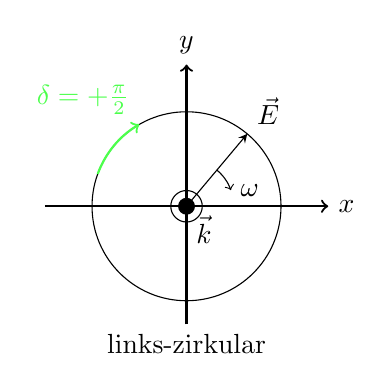
\begin{tikzpicture}[]
	% Achsen zeichnen
	\draw[->,thick] (-1.8,0) -- (1.8,0) node[right] {$x$};
	\draw[->,thick] (0,-1.5) -- (0,1.8) node[above] {$y$};
	%Plot
	%\draw[style=dashed] (-1.27,-1.05) rectangle (1.27,1.05);
	\draw (0, 0) circle (1.2);
	\draw (0, 0) circle (.2);
	\draw[fill=black] (0, 0) circle (.1);
	\draw (0,0) node[below right] {$\vec{k}$};
	\draw[->,>=stealth] (0,0)--(50:1.2) node[above right] {$\vec{E}$};
	\draw[->] (50:.6) arc (50:20:.6) node [right] {$\omega$};
	\draw [->,thick,color=green!70] (160:1.2) arc (160:120:1.2) node[above left] {$\delta = +\frac{\pi}{2}$};
	\draw (0,-1.5) node[below]{links-zirkular};
\end{tikzpicture}
		        \end{center}

		  Di \textbf{Überlagerung} zweier links und rechts umlaufender zirkular polarisierter Wellen (\textbf{unterschiedlicher Amplitude}) ergibt wieder eine \textbf{beliebig polarisierte Welle}. Bei \textbf{gleicher Amplitude} ist die resultierende Welle \textbf{linear polarisiert}.
  \subsubsection{3. Fall: Elliptische Polarisation}
	  Weiter wird \(\delta = (2m+1) \frac{\pi}{2}, \quad m \in \mathbb{Z} , \quad\delta = \pm \frac{\pi}{2}, \pm \frac{3\pi}{2},\ldots \quad ;\quad\vert E_{0x} \vert \neq \vert E_{0y} \vert  \) untersucht. Analog zur zirkularen Polarisation folgt für das elektrische Feld:
		        \begin{equation}\begin{split}
				        E_x &= \vert E_{0x} \vert \cos (\omega t -  k r + \varphi_x)\\
				        E_y &= \mp \vert E_{0y} \vert \sin (\omega t -  k r + \varphi_x) \quad (\textcolor{red}{+},\textcolor{green}{-})\\
				        \Rightarrow &\left[ \frac{E_x}{\vert \ubar{E}_{0x}\vert}\right]^2+\left[\frac{E_y}{\vert \ubar{E}_{0y}\vert}\right]^2 = 1\quad
			        \end{split}\end{equation}
		Durch diese Gleichung wird eine Ellipse mit den Halbachsen $\vert E_{0x} \vert , \vert E_{0y} \vert$ beschrieben. Man spricht deshalb von einer (rechts- bzw. linksumlaufenden) \textbf{elliptisch polarisierten Welle}. Visualisierung:
		        \begin{center}
			        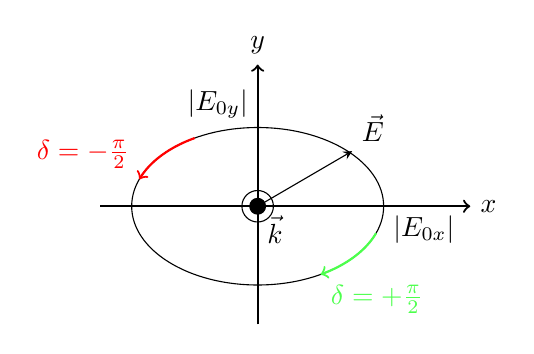
\begin{tikzpicture}
	% Achsen zeichnen
	\draw[->,thick] (-2,0) -- (2.7,0) node[right] {$x$};
	\draw[->,thick] (0,-1.5) -- (0,1.8) node[above] {$y$};
	%Plot
	%\draw[style=dashed] (-1.27,-1.05) rectangle (1.27,1.05);
	\draw (0, 0) ellipse (1.6 and 1);
	\draw(1.6,0) node[below right] {$|E_{0x}|$} ;
	\draw(0,1.3) node[left] {$|E_{0y}|$} ;
	\draw[->,>=stealth] (0,0)--(1.2,0.7) node[above right] {$\vec{E}$};
	%\draw[->,color=green] (40:1) arc (40:160:1.3);
	\draw [->,thick,color=green!70] plot[domain=340:300] ({cos(\x)*1.6},{sin(\x)}) node[below right] {$\delta = +\frac{\pi}{2}$};
	\draw [->,thick,color=red] plot[domain=120:160] ({cos(\x)*1.6},{sin(\x)}) node[above left] {$\delta = -\frac{\pi}{2}$};
	\draw (0, 0) circle (.2);
	\draw[fill=black] (0, 0) circle (.1);
	\draw (0,0) node[below right] {$\vec{k}$};
\end{tikzpicture}
		        \end{center}
  \subsubsection{4. Fall: keine Einschränkungen}
		  Abschließend gibt es keine Einschränkungen für \(\delta\) und \(\vert E_{0x} \vert\) bzw. \(\vert E_{0y} \vert  \) mehr. Analog zur zirkularen Polarisation folgt ohne weitere Herleitung:
		        \begin{itemize}
			        \item Das Ergebnis ist \textbf{elliptisch polarisiert} (Stichwort: \href{https://en.wikipedia.org/wiki/Jones_calculus}{Jones-Vektor}).
			        \item Die Halbachsen sind gegen das \(x\)-\(y\)-System gedreht.
			              \begin{center}
				              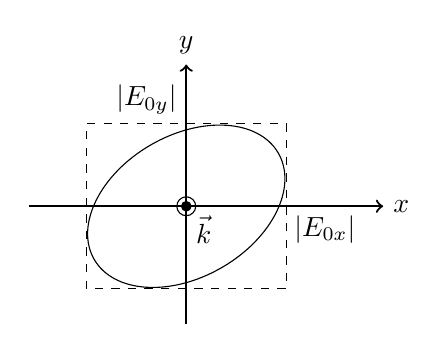
\begin{tikzpicture}
	% Achsen zeichnen
	\draw[->,thick] (-2,0) -- (2.5,0) node[right] {$x$};
	\draw[->,thick] (0,-1.5) -- (0,1.8) node[above] {$y$};
	%Plot
	\draw[style=dashed] (-1.27,-1.05) rectangle (1.27,1.05);
	\draw[rotate=30] (0, 0) ellipse (1.35 and 0.9);
	\draw(1.25,0) node[below right] {$|E_{0x}|$} ;
	\draw(0,1.05) node[above left] {$|E_{0y}|$} ;
	\draw (0, 0) circle (.12);
	\draw[fill=black] (0, 0) circle (.06);
	\draw (0,0) node[below right] {$\vec{k}$};
\end{tikzpicture}
			              \end{center}
		        \end{itemize}
		       Eine beliebige Polarisation lässt sich zusammensetzen aus:
		        \begin{itemize}
			        \item 2 linear polarisierten Wellen, die zueinander senkrecht stehen
			        \item 2 zirkular polarisierten Wellen, die entgegenlaufend sind
		        \end{itemize}
		        \href{https://emanim.szialab.org}{Online-Visualisierung.}
 \subsection{Wellenpakete}
 \subsubsection{Polychromatische Wellen}
 Die ebenen Wellen, die sich in den Wellenpaketen bewegen, können beliebig polarisiert sein. Für die Anschauung kann man von linearer Polarisation ausgehen, denn aus der Überlagerung von 2 linear polarisierten Wellen, die zueinander senkrecht stehen lässt sich eine beliebige Polarisation herleiten. Weiter werden Lösungen der homogenen Wellengleichung ($\nearrow$\ref{homwell}) betrachtet. Lösungen, die sich nur in einer Richtung (aber hin- und rücklaufend) ausbreiten, haben die allgemeine Form der ebenen Welle aus Gleichung \ref{algebwell}. Eine alternative Schreibweise betrachtet die Überlagerung für verschiedene Wellenvektoren (\(\vec{k} =  k\; \vu{k} = \omega\sqrt{\varepsilon\mu}\;\vu{k}\to\) $k$ und $\omega$ hängen zusammen, nun Überlagerung der $k$). $k$ und $\omega$ sind kontinuierlich, deshalb ist die folgende integrale Schreibweise sinnvoll:
		        \begin{equation}
			        \boxed{\Psi (\vec{r} , t) = \int\limits_{0}^\infty \left[ A_+(k) \Psi_+ (\omega t + \vec{k}\cdot\vec{r} ) + A_-(k) \Psi_- (\omega t - \vec{k}\cdot\vec{r} ) \right] \dd  k}
		        \end{equation}
		        Solch eine Überlagerung für verschiedene $k$ (und damit für verschiedene $\omega$) nennt man \textbf{polychromatische Welle}. Hier sind zudem die expliziten Vorfaktoren eingeführt, die homogenen Lösungen können mit beliebigen Konstanten gewichtet überlagert werden und bilden immer noch eine homogene Lösung. Außerdem wurde in \ref{algebwell} das Integral als Summe geschrieben (obwohl es sich um kontinuierliche Variablen handelt). 
		   Ohne Beschränkung der Allgemeinheit kann \(\vec{k} =  k \vu{z}   \implies \vec{k}\cdot\vec{r}  =  k z\), also eine Ausbreitung entlang der \(z\)-Richtung angenommen werden.
  \subsubsection{Dispersion}
 In der Regel sind die Materialparameter \textbf{frequenzabhängig}:
		        \begin{align}
			        \varepsilon & = \varepsilon_0\varepsilon_r = \varepsilon_0\varepsilon_r(\omega) & \mu & = \mu_0\mu_r = \mu_0\mu_r(\omega)
		        \end{align}
Somit haben \textbf{Teilwellen unterschiedliche Phasengeschwindigkeiten}:
		        \begin{equation}
			        v_\mathrm{p} (\omega) =  v_\mathrm{c}(\omega) = \frac{1}{\sqrt{\varepsilon\mu}} = \frac{1}{\sqrt{\varepsilon_0\mu_0}} \frac{1}{\sqrt{\varepsilon_r(\omega)\mu_r(\omega)}}=\frac{c}{n(\omega)}
		        \end{equation}
Dies tritt insbesondere bei \textbf{Wellenpaketen} in Erscheinung. Unter einem Wellenpaket mit \textbf{harmonischer Zeitabhängigkeit}, das in \textbf{\(+z\)-Richtung} propagiert, versteht man eine Überlagerung der Form
		        \begin{equation}
			        \Psi (\vec{r} , t) = \int\limits_{-\infty}^\infty \underline{A}(k) \mathrm{e}^{\mathrm{j}(\omega t -  k z)} \dd  k\; , \text{ mit } \underline{A}(-k) = \underline{A}^\star(k)
		        \end{equation}
		  Ein häufiger Spezialfall ist $\underline{A}(k) = A(k)$ reelwertig mit $A(-k) = A(k)$. Hierbei soll \(A(k)\) zunächst \textbf{konzentriert} sein um \( k =  k_0\), also:
		        \begin{center}
			        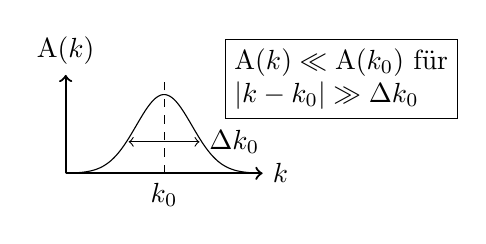
\begin{tikzpicture}[scale=0.5, samples=200, domain=0:5]
	% Achsen zeichnen
	\draw[->,thick] (0,0) -- (5,0) node[right] {$ k$};
	\draw[->,thick] (0,0) -- (0,2.5) node[above] {$\mathrm{A}( k)$};
	%Plot
	\draw plot (\x,{exp(-(\x-2.5)^2)*2});
	\draw [style=dashed] (2.5,0) node[below] {$ k_0$} --(2.5,2.4);
	\draw[<->] (1.6,.8)--(3.4,.8) node[right] {$\Delta  k_0$};
	\node[draw,align=left] at (7,2.4) {$\mathrm{A}( k) \ll \mathrm{A}( k_0)$ für\\ $| k- k_0| \gg \Delta  k_0$};
\end{tikzpicture}
		        \end{center}
		   Da die Wichtungsfunktion \(A( k)\) um \( k =  k_0\) konzentriert ist, bietet sich eine \textbf{Taylorentwicklung} von \(\omega( k)\) um \( k_0\) an, in den Bereichen nahe $k_0$ approximiert diese \(\omega( k)\) gut.
		        \begin{align}
			        \omega( k) & = \omega( k_0) + \left.\frac{\dd \omega}{\dd  k}\right|_{ k_0} ( k -  k_0) + \ldots                                                                                                                                          \\
			                   & \cong \underbrace{\omega( k_0)}_{=\omega_0} +  v_{\mathrm{g}}( k- k_0)              & \rightarrow\boxed{ v_{\mathrm{g}} = \left.\frac{\dd \omega}{\dd  k}\right|_{ k_0}}
		        \end{align}
		        $v_{\mathrm{g}}$ wird dabei \textbf{Gruppengeschwindigkeit} genannt.
		   Den Verlauf \(\omega( k)\) nennt man auch \textbf{Dispersionsrelation}. Es gilt allgemein $k=\omega\sqrt{\mu(\omega)\varepsilon(\omega)}$, praktisch leitet man $\omega(k)$ selten mikroskopisch her, sondern setzt Modelle an. Bei bestimmten Dispersionsrelationen kann es auch negative Gruppengeschwindigkeiten für bestimmte $k$ geben. Wenn man einen Puls auf ein Material mit einer solchen Relation gibt, kann ein Maximum in positive und eines in negative Richtung propagieren. Im Fall von Dispersion (bei negativen Gruppengeschwindigkeiten würde die Kurve auch monoton falled) resultiert die linke Grafik, im Fall ohne Dispersion die rechte Grafik.
		  
		        \begin{center}
			        \begin{tikzpicture}[domain=0:2.5]
	% Achsen zeichnen
	\draw[->,thick] (0,0) -- (5,0) node[right] {$ k$};
	\draw[->,thick] (0,0) -- (0,3) node[above] {$\omega( k)$};
	%Plot
	\draw plot (\x,{0.2*exp(\x)-0.2});
	% Beschriftung
	\draw (-.1,1.25) -- (.1,1.25) node[left=4pt] {$\omega_0$};
	\draw (2,-.1) -- (2,.1) node[below=4pt] {$ k_0$};
	\draw[style=dashed] (.2,1.25)--(2,1.25) node[right=8pt] {$ v_{\mathrm{g}}$} -- (2, .2);
	\draw (1.25,0.25)--(2.75,2.25);
\end{tikzpicture}
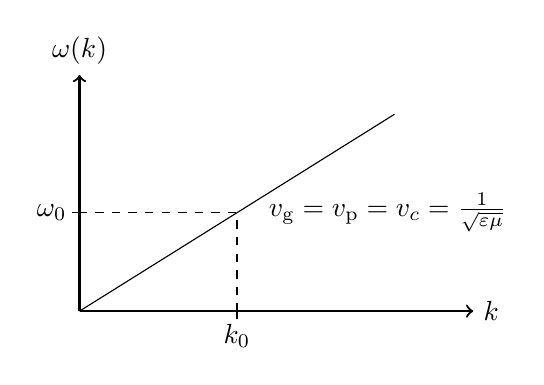
\begin{tikzpicture}
	% Achsen zeichnen
	\draw[->,thick] (0,0) -- (5,0) node[right] {$ k$};
	\draw[->,thick] (0,0) -- (0,3) node[above] {$\omega( k)$};
	% Plott
	\draw (0,0) -- (4,2.5);
	% Beschriftung
	\draw (-.1,1.25) -- (.1,1.25) node[left=4pt] {$\omega_0$};
	\draw (2,-.1) -- (2,.1) node[below=4pt] {$ k_0$};
	\draw[style=dashed] (.2,1.25)--(2,1.25)node[right=8pt] {$ v_{\mathrm{g}}= v_{\mathrm{p}}= v_{c} = \frac{1}{\sqrt{\varepsilon\mu}}$} -- (2, .2);
\end{tikzpicture}
		        \end{center}
		        Allgemein gilt bei ebenen Wellen immer $v_{\mathrm{c}}=v_{\mathrm{p}}$, aber nicht $v_{\mathrm{g}}=v_{\mathrm{c}}$. Das Phänomen der Frequenzabhängigkeit der Phasengeschwindigkeit heißt \textbf{Dispersion}. 
  \subsubsection{Dispersion von Wellenpaketen}
	  Die Taylor-Entwicklung kann man in e-Funktion einsetzen:
		        \begin{equation}
			        \mathrm{e}^{\mathrm{j}(\omega t -  k z)} \cong  \mathrm{e}^{\mathrm{j}(\omega_0 t -  k_0 z)}  \mathrm{e}^{\mathrm{j}(\overbrace{ k -  k_0}^{=q})( v_{\mathrm{g}} t - z)}
		        \end{equation}
		Damit folgt für das Wellenpaket:
		        \begin{equation}\begin{split}
				        \Psi (\vec{r} , t) &\cong \underbrace{\int\limits_{-\infty}^{\infty} \underbrace{A( k_0 + q)}_{A( k)} \mathrm{e}^{\mathrm{j}q ( v_{\mathrm{g}} t - z)}\dd q}_{\mathrm{H}( v_{\mathrm{g}} t -z)} \cdot\;  \mathrm{e}^{\mathrm{j}( \omega_0 t -  k_0 z)}\\
				        & \cong \underbrace{\mathrm{H}( v_{\mathrm{g}} t -z)}_{\substack{\text{Einhüllende}\\ \text{propagiert mit } v_{\mathrm{g}}\\ \text{in Richtung $z$}}}\cdot\; \underbrace{ \mathrm{e}^{\mathrm{j}(\omega_0 t -  k_0 z)}}_{\substack{\text{ebene Welle,}\\ \omega = \omega_0\\  k =  k_0}}
			        \end{split}\end{equation}
		        Für die konzentrierte Wichtungsfunktion resultiert also eine Hüllkurve, die mit $v_{\mathrm{g}}$ in $z$-Richtung propagiert und \textbf{eine} (durch die Linearisierung) ebene Welle. Visuell sieht man, dass die Phasengeschwindigkeit von der Gruppengeschwindigkeit abweicht (die Maxima von roter und blauer kurve sind bei $t_2$ gegeneinander verschoben):
	  \begin{center}
		  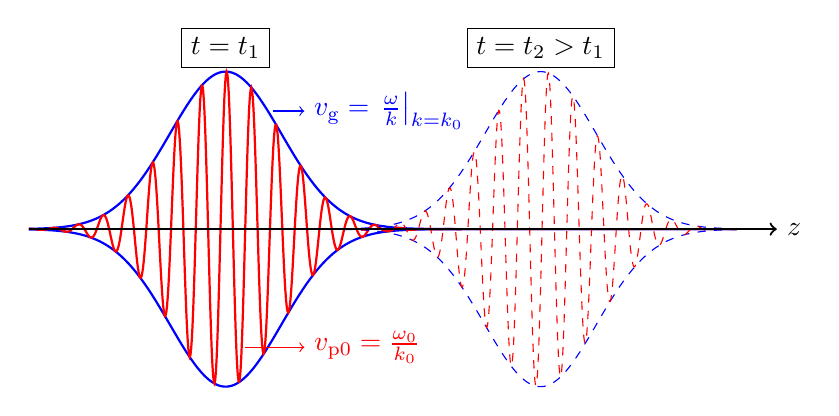
\begin{tikzpicture}[samples=1000, domain=0:9]
	%Plotten
	\draw [color=blue, thick] plot (\x,{exp(-(\x-2.5)^2)*2});
	\draw [color=blue, thick] plot (\x,{-exp(-(\x-2.5)^2)*2});
	\draw [color=red, thick] plot (\x,{cos(deg(\x*20))*exp(-(\x-2.5)^2)*2});

	\draw [style=dashed, color=blue] plot (\x,{exp(-(\x-6.5)^2)*2});
	\draw [style=dashed, color=blue] plot (\x,{-exp(-(\x-6.5)^2)*2});
	\draw [style=dashed, color=red] plot (\x,{cos(deg(\x*20))*exp(-(\x-6.5)^2)*2});

	%\draw[color=red] (0.5,0) sin(0.7,0.5) cos(0.9,0) sin(1.1,-0.66) cos(1.3,0) sin(1.5,1) cos(1.7,0) sin(1.9,-1.37) cos(2.1,0) sin(2.3,1.8) cos(2.5,0) sin(2.7,-2.15) cos(2.9,0) sin(3.1,2.38) cos(3.3,0) sin(3.5,-2.5) cos(3.7,0) sin(3.9,2.38) cos(4.1,0) sin(4.3,-2.15) cos(4.5,0) sin(4.7,1.8) cos(4.9,0) sin(5.1,-1.37) cos(5.3,0) sin(5.5,1) cos(5.7,0) sin(5.9,-0.66) cos(6.1,0) sin(6.3,0.5) cos(6.5,0);
	%\draw (0.5,0.5) cos(2,1.5) sin(3.5,2.5) cos(5,1.5) sin(6.5,0.5);% cos (8,0);
	%\draw (0.5,-0.5) cos(2,-1.5) sin(3.5,-2.5) cos(5,-1.5) sin(6.5,-0.5);% cos (8,0);
	% \begin{axis}
	%        \addplot[samples=500,domain=0:180]{sin(x)*2*sin(20*x)};%x in degrees, 500 samples into the domain
	% \end{axis}

	%Beschriftung
	\draw[->, color=blue] (3.1,1.5)--(3.5,1.5) node[right] {$ v_{\mathrm{g}}=\left.\frac{\dd \omega}{\dd  k}\right|_{ k= k_0}$};
	\draw[->, color=red] (2.75,-1.5)--(3.5,-1.5) node[right] {$ v_{\mathrm{p0}}=\frac{\omega_0}{ k_0}$};
	\node[draw] at (2.5,2.3) {$t=t_1$};
	\node[draw] at (6.5,2.3) {$t=t_2>t_1$};
	% Achse zeichnen
	\draw[->,thick] (0,0) -- (9.5,0) node[right] {$z$};
\end{tikzpicture}
	  \end{center}
		  Die Dispersionsrelation \(\omega( k)\) wurde um \(\omega_0\) nach Taylor bis zur ersten Ordung entwickelt (\textbf{linearisiert}) und so das Wellenpaket mit Einhüllender und Träger erhalten. Aus der Herleitung ist klar, dass das ganze nur sinnvoll ist, wenn \(A(k)\) um \(k_0\) \textbf{konzentriert} ist. Die Taylor-Approximation ist dann für $k$ mit großer Amplitude (also für einen Großteil des Signals im Sinne von Energie) gut. Bei breitbandiger Überlagerung enthält das Wellenpaket viele Frequenzanteile, die in der Regel alle mit \textbf{unterschiedlicher Phasengeschwindigkeit} \( v_\mathrm{p}(\omega)\) propagieren, eine Taylor-Entwicklung um den Konzentrationspunkt ist hier nicht sinnvoll. Die Form der Einhüllenden verändert sich durch die unterschiedlichen Phasengeschwindigkeiten. Auch dies wird häufig \textbf{Dispersion} genannt. Das \textbf{Zerfließen} eines Wellenpakets (Signals) ist eine wichtige Begrenzung beim technischen Einsatz (z.B. Signalübertragung über lange Distanzen in Glasfaser-Kabeln). Die folgende Grafik ist auch als \href{https://github.com/hgkdd/TET/tree/main/programs/wave_packet_dispersion}{Animation} verfügbar. Man erkennt, dass das Wellenpaket im Fall einer konstanten Phasengeschwindigkeit, also einem tatsächlich linearen $\omega(k)-$Zusammenhang, nicht zerfließt. Die Linearisierung ist in diesem Fall exakt. Bei einer nicht konstanten Phasengeschwindigkeit (hier abgebildet) ist das Zerfließen zu erkennen.
	  \begin{center}
		  \resizebox{0.6\textwidth}{!}{%% Creator: Matplotlib, PGF backend
%%
%% To include the figure in your LaTeX document, write
%%   \input{<filename>.pgf}
%%
%% Make sure the required packages are loaded in your preamble
%%   \usepackage{pgf}
%%
%% Also ensure that all the required font packages are loaded; for instance,
%% the lmodern package is sometimes necessary when using math font.
%%   \usepackage{lmodern}
%%
%% Figures using additional raster images can only be included by \input if
%% they are in the same directory as the main LaTeX file. For loading figures
%% from other directories you can use the `import` package
%%   \usepackage{import}
%%
%% and then include the figures with
%%   \import{<path to file>}{<filename>.pgf}
%%
%% Matplotlib used the following preamble
%%   
%%   \usepackage{fontspec}
%%   
%%   \makeatletter\@ifpackageloaded{underscore}{}{\usepackage[strings]{underscore}}\makeatother
%%
\begingroup%
\makeatletter%
\begin{pgfpicture}%
\pgfpathrectangle{\pgfpointorigin}{\pgfqpoint{5.952826in}{4.370365in}}%
\pgfusepath{use as bounding box, clip}%
\begin{pgfscope}%
\pgfsetbuttcap%
\pgfsetmiterjoin%
\pgfsetlinewidth{0.000000pt}%
\definecolor{currentstroke}{rgb}{0.000000,0.000000,0.000000}%
\pgfsetstrokecolor{currentstroke}%
\pgfsetstrokeopacity{0.000000}%
\pgfsetdash{}{0pt}%
\pgfpathmoveto{\pgfqpoint{0.000000in}{0.000000in}}%
\pgfpathlineto{\pgfqpoint{5.952826in}{0.000000in}}%
\pgfpathlineto{\pgfqpoint{5.952826in}{4.370365in}}%
\pgfpathlineto{\pgfqpoint{0.000000in}{4.370365in}}%
\pgfpathlineto{\pgfqpoint{0.000000in}{0.000000in}}%
\pgfpathclose%
\pgfusepath{}%
\end{pgfscope}%
\begin{pgfscope}%
\pgfsetbuttcap%
\pgfsetmiterjoin%
\pgfsetlinewidth{0.000000pt}%
\definecolor{currentstroke}{rgb}{0.000000,0.000000,0.000000}%
\pgfsetstrokecolor{currentstroke}%
\pgfsetstrokeopacity{0.000000}%
\pgfsetdash{}{0pt}%
\pgfpathmoveto{\pgfqpoint{0.804460in}{0.521603in}}%
\pgfpathlineto{\pgfqpoint{5.764460in}{0.521603in}}%
\pgfpathlineto{\pgfqpoint{5.764460in}{4.217603in}}%
\pgfpathlineto{\pgfqpoint{0.804460in}{4.217603in}}%
\pgfpathlineto{\pgfqpoint{0.804460in}{0.521603in}}%
\pgfpathclose%
\pgfusepath{}%
\end{pgfscope}%
\begin{pgfscope}%
\pgfpathrectangle{\pgfqpoint{0.804460in}{0.521603in}}{\pgfqpoint{4.960000in}{3.696000in}}%
\pgfusepath{clip}%
\pgfsetrectcap%
\pgfsetroundjoin%
\pgfsetlinewidth{0.803000pt}%
\definecolor{currentstroke}{rgb}{0.690196,0.690196,0.690196}%
\pgfsetstrokecolor{currentstroke}%
\pgfsetdash{}{0pt}%
\pgfpathmoveto{\pgfqpoint{0.804460in}{0.521603in}}%
\pgfpathlineto{\pgfqpoint{0.804460in}{4.217603in}}%
\pgfusepath{stroke}%
\end{pgfscope}%
\begin{pgfscope}%
\pgfsetbuttcap%
\pgfsetroundjoin%
\definecolor{currentfill}{rgb}{0.000000,0.000000,0.000000}%
\pgfsetfillcolor{currentfill}%
\pgfsetlinewidth{0.803000pt}%
\definecolor{currentstroke}{rgb}{0.000000,0.000000,0.000000}%
\pgfsetstrokecolor{currentstroke}%
\pgfsetdash{}{0pt}%
\pgfsys@defobject{currentmarker}{\pgfqpoint{0.000000in}{-0.048611in}}{\pgfqpoint{0.000000in}{0.000000in}}{%
\pgfpathmoveto{\pgfqpoint{0.000000in}{0.000000in}}%
\pgfpathlineto{\pgfqpoint{0.000000in}{-0.048611in}}%
\pgfusepath{stroke,fill}%
}%
\begin{pgfscope}%
\pgfsys@transformshift{0.804460in}{0.521603in}%
\pgfsys@useobject{currentmarker}{}%
\end{pgfscope}%
\end{pgfscope}%
\begin{pgfscope}%
\definecolor{textcolor}{rgb}{0.000000,0.000000,0.000000}%
\pgfsetstrokecolor{textcolor}%
\pgfsetfillcolor{textcolor}%
\pgftext[x=0.804460in,y=0.424381in,,top]{\color{textcolor} \fontsize{10.000000}{12.000000}\selectfont \ensuremath{-}5}%
\end{pgfscope}%
\begin{pgfscope}%
\pgfpathrectangle{\pgfqpoint{0.804460in}{0.521603in}}{\pgfqpoint{4.960000in}{3.696000in}}%
\pgfusepath{clip}%
\pgfsetrectcap%
\pgfsetroundjoin%
\pgfsetlinewidth{0.803000pt}%
\definecolor{currentstroke}{rgb}{0.690196,0.690196,0.690196}%
\pgfsetstrokecolor{currentstroke}%
\pgfsetdash{}{0pt}%
\pgfpathmoveto{\pgfqpoint{1.513032in}{0.521603in}}%
\pgfpathlineto{\pgfqpoint{1.513032in}{4.217603in}}%
\pgfusepath{stroke}%
\end{pgfscope}%
\begin{pgfscope}%
\pgfsetbuttcap%
\pgfsetroundjoin%
\definecolor{currentfill}{rgb}{0.000000,0.000000,0.000000}%
\pgfsetfillcolor{currentfill}%
\pgfsetlinewidth{0.803000pt}%
\definecolor{currentstroke}{rgb}{0.000000,0.000000,0.000000}%
\pgfsetstrokecolor{currentstroke}%
\pgfsetdash{}{0pt}%
\pgfsys@defobject{currentmarker}{\pgfqpoint{0.000000in}{-0.048611in}}{\pgfqpoint{0.000000in}{0.000000in}}{%
\pgfpathmoveto{\pgfqpoint{0.000000in}{0.000000in}}%
\pgfpathlineto{\pgfqpoint{0.000000in}{-0.048611in}}%
\pgfusepath{stroke,fill}%
}%
\begin{pgfscope}%
\pgfsys@transformshift{1.513032in}{0.521603in}%
\pgfsys@useobject{currentmarker}{}%
\end{pgfscope}%
\end{pgfscope}%
\begin{pgfscope}%
\definecolor{textcolor}{rgb}{0.000000,0.000000,0.000000}%
\pgfsetstrokecolor{textcolor}%
\pgfsetfillcolor{textcolor}%
\pgftext[x=1.513032in,y=0.424381in,,top]{\color{textcolor} \fontsize{10.000000}{12.000000}\selectfont 0}%
\end{pgfscope}%
\begin{pgfscope}%
\pgfpathrectangle{\pgfqpoint{0.804460in}{0.521603in}}{\pgfqpoint{4.960000in}{3.696000in}}%
\pgfusepath{clip}%
\pgfsetrectcap%
\pgfsetroundjoin%
\pgfsetlinewidth{0.803000pt}%
\definecolor{currentstroke}{rgb}{0.690196,0.690196,0.690196}%
\pgfsetstrokecolor{currentstroke}%
\pgfsetdash{}{0pt}%
\pgfpathmoveto{\pgfqpoint{2.221603in}{0.521603in}}%
\pgfpathlineto{\pgfqpoint{2.221603in}{4.217603in}}%
\pgfusepath{stroke}%
\end{pgfscope}%
\begin{pgfscope}%
\pgfsetbuttcap%
\pgfsetroundjoin%
\definecolor{currentfill}{rgb}{0.000000,0.000000,0.000000}%
\pgfsetfillcolor{currentfill}%
\pgfsetlinewidth{0.803000pt}%
\definecolor{currentstroke}{rgb}{0.000000,0.000000,0.000000}%
\pgfsetstrokecolor{currentstroke}%
\pgfsetdash{}{0pt}%
\pgfsys@defobject{currentmarker}{\pgfqpoint{0.000000in}{-0.048611in}}{\pgfqpoint{0.000000in}{0.000000in}}{%
\pgfpathmoveto{\pgfqpoint{0.000000in}{0.000000in}}%
\pgfpathlineto{\pgfqpoint{0.000000in}{-0.048611in}}%
\pgfusepath{stroke,fill}%
}%
\begin{pgfscope}%
\pgfsys@transformshift{2.221603in}{0.521603in}%
\pgfsys@useobject{currentmarker}{}%
\end{pgfscope}%
\end{pgfscope}%
\begin{pgfscope}%
\definecolor{textcolor}{rgb}{0.000000,0.000000,0.000000}%
\pgfsetstrokecolor{textcolor}%
\pgfsetfillcolor{textcolor}%
\pgftext[x=2.221603in,y=0.424381in,,top]{\color{textcolor}\fontsize{10.000000}{12.000000}\selectfont 5}%
\end{pgfscope}%
\begin{pgfscope}%
\pgfpathrectangle{\pgfqpoint{0.804460in}{0.521603in}}{\pgfqpoint{4.960000in}{3.696000in}}%
\pgfusepath{clip}%
\pgfsetrectcap%
\pgfsetroundjoin%
\pgfsetlinewidth{0.803000pt}%
\definecolor{currentstroke}{rgb}{0.690196,0.690196,0.690196}%
\pgfsetstrokecolor{currentstroke}%
\pgfsetdash{}{0pt}%
\pgfpathmoveto{\pgfqpoint{2.930175in}{0.521603in}}%
\pgfpathlineto{\pgfqpoint{2.930175in}{4.217603in}}%
\pgfusepath{stroke}%
\end{pgfscope}%
\begin{pgfscope}%
\pgfsetbuttcap%
\pgfsetroundjoin%
\definecolor{currentfill}{rgb}{0.000000,0.000000,0.000000}%
\pgfsetfillcolor{currentfill}%
\pgfsetlinewidth{0.803000pt}%
\definecolor{currentstroke}{rgb}{0.000000,0.000000,0.000000}%
\pgfsetstrokecolor{currentstroke}%
\pgfsetdash{}{0pt}%
\pgfsys@defobject{currentmarker}{\pgfqpoint{0.000000in}{-0.048611in}}{\pgfqpoint{0.000000in}{0.000000in}}{%
\pgfpathmoveto{\pgfqpoint{0.000000in}{0.000000in}}%
\pgfpathlineto{\pgfqpoint{0.000000in}{-0.048611in}}%
\pgfusepath{stroke,fill}%
}%
\begin{pgfscope}%
\pgfsys@transformshift{2.930175in}{0.521603in}%
\pgfsys@useobject{currentmarker}{}%
\end{pgfscope}%
\end{pgfscope}%
\begin{pgfscope}%
\definecolor{textcolor}{rgb}{0.000000,0.000000,0.000000}%
\pgfsetstrokecolor{textcolor}%
\pgfsetfillcolor{textcolor}%
\pgftext[x=2.930175in,y=0.424381in,,top]{\color{textcolor}\fontsize{10.000000}{12.000000}\selectfont 10}%
\end{pgfscope}%
\begin{pgfscope}%
\pgfpathrectangle{\pgfqpoint{0.804460in}{0.521603in}}{\pgfqpoint{4.960000in}{3.696000in}}%
\pgfusepath{clip}%
\pgfsetrectcap%
\pgfsetroundjoin%
\pgfsetlinewidth{0.803000pt}%
\definecolor{currentstroke}{rgb}{0.690196,0.690196,0.690196}%
\pgfsetstrokecolor{currentstroke}%
\pgfsetdash{}{0pt}%
\pgfpathmoveto{\pgfqpoint{3.638746in}{0.521603in}}%
\pgfpathlineto{\pgfqpoint{3.638746in}{4.217603in}}%
\pgfusepath{stroke}%
\end{pgfscope}%
\begin{pgfscope}%
\pgfsetbuttcap%
\pgfsetroundjoin%
\definecolor{currentfill}{rgb}{0.000000,0.000000,0.000000}%
\pgfsetfillcolor{currentfill}%
\pgfsetlinewidth{0.803000pt}%
\definecolor{currentstroke}{rgb}{0.000000,0.000000,0.000000}%
\pgfsetstrokecolor{currentstroke}%
\pgfsetdash{}{0pt}%
\pgfsys@defobject{currentmarker}{\pgfqpoint{0.000000in}{-0.048611in}}{\pgfqpoint{0.000000in}{0.000000in}}{%
\pgfpathmoveto{\pgfqpoint{0.000000in}{0.000000in}}%
\pgfpathlineto{\pgfqpoint{0.000000in}{-0.048611in}}%
\pgfusepath{stroke,fill}%
}%
\begin{pgfscope}%
\pgfsys@transformshift{3.638746in}{0.521603in}%
\pgfsys@useobject{currentmarker}{}%
\end{pgfscope}%
\end{pgfscope}%
\begin{pgfscope}%
\definecolor{textcolor}{rgb}{0.000000,0.000000,0.000000}%
\pgfsetstrokecolor{textcolor}%
\pgfsetfillcolor{textcolor}%
\pgftext[x=3.638746in,y=0.424381in,,top]{\color{textcolor}\fontsize{10.000000}{12.000000}\selectfont 15}%
\end{pgfscope}%
\begin{pgfscope}%
\pgfpathrectangle{\pgfqpoint{0.804460in}{0.521603in}}{\pgfqpoint{4.960000in}{3.696000in}}%
\pgfusepath{clip}%
\pgfsetrectcap%
\pgfsetroundjoin%
\pgfsetlinewidth{0.803000pt}%
\definecolor{currentstroke}{rgb}{0.690196,0.690196,0.690196}%
\pgfsetstrokecolor{currentstroke}%
\pgfsetdash{}{0pt}%
\pgfpathmoveto{\pgfqpoint{4.347318in}{0.521603in}}%
\pgfpathlineto{\pgfqpoint{4.347318in}{4.217603in}}%
\pgfusepath{stroke}%
\end{pgfscope}%
\begin{pgfscope}%
\pgfsetbuttcap%
\pgfsetroundjoin%
\definecolor{currentfill}{rgb}{0.000000,0.000000,0.000000}%
\pgfsetfillcolor{currentfill}%
\pgfsetlinewidth{0.803000pt}%
\definecolor{currentstroke}{rgb}{0.000000,0.000000,0.000000}%
\pgfsetstrokecolor{currentstroke}%
\pgfsetdash{}{0pt}%
\pgfsys@defobject{currentmarker}{\pgfqpoint{0.000000in}{-0.048611in}}{\pgfqpoint{0.000000in}{0.000000in}}{%
\pgfpathmoveto{\pgfqpoint{0.000000in}{0.000000in}}%
\pgfpathlineto{\pgfqpoint{0.000000in}{-0.048611in}}%
\pgfusepath{stroke,fill}%
}%
\begin{pgfscope}%
\pgfsys@transformshift{4.347318in}{0.521603in}%
\pgfsys@useobject{currentmarker}{}%
\end{pgfscope}%
\end{pgfscope}%
\begin{pgfscope}%
\definecolor{textcolor}{rgb}{0.000000,0.000000,0.000000}%
\pgfsetstrokecolor{textcolor}%
\pgfsetfillcolor{textcolor}%
\pgftext[x=4.347318in,y=0.424381in,,top]{\color{textcolor}\fontsize{10.000000}{12.000000}\selectfont 20}%
\end{pgfscope}%
\begin{pgfscope}%
\pgfpathrectangle{\pgfqpoint{0.804460in}{0.521603in}}{\pgfqpoint{4.960000in}{3.696000in}}%
\pgfusepath{clip}%
\pgfsetrectcap%
\pgfsetroundjoin%
\pgfsetlinewidth{0.803000pt}%
\definecolor{currentstroke}{rgb}{0.690196,0.690196,0.690196}%
\pgfsetstrokecolor{currentstroke}%
\pgfsetdash{}{0pt}%
\pgfpathmoveto{\pgfqpoint{5.055889in}{0.521603in}}%
\pgfpathlineto{\pgfqpoint{5.055889in}{4.217603in}}%
\pgfusepath{stroke}%
\end{pgfscope}%
\begin{pgfscope}%
\pgfsetbuttcap%
\pgfsetroundjoin%
\definecolor{currentfill}{rgb}{0.000000,0.000000,0.000000}%
\pgfsetfillcolor{currentfill}%
\pgfsetlinewidth{0.803000pt}%
\definecolor{currentstroke}{rgb}{0.000000,0.000000,0.000000}%
\pgfsetstrokecolor{currentstroke}%
\pgfsetdash{}{0pt}%
\pgfsys@defobject{currentmarker}{\pgfqpoint{0.000000in}{-0.048611in}}{\pgfqpoint{0.000000in}{0.000000in}}{%
\pgfpathmoveto{\pgfqpoint{0.000000in}{0.000000in}}%
\pgfpathlineto{\pgfqpoint{0.000000in}{-0.048611in}}%
\pgfusepath{stroke,fill}%
}%
\begin{pgfscope}%
\pgfsys@transformshift{5.055889in}{0.521603in}%
\pgfsys@useobject{currentmarker}{}%
\end{pgfscope}%
\end{pgfscope}%
\begin{pgfscope}%
\definecolor{textcolor}{rgb}{0.000000,0.000000,0.000000}%
\pgfsetstrokecolor{textcolor}%
\pgfsetfillcolor{textcolor}%
\pgftext[x=5.055889in,y=0.424381in,,top]{\color{textcolor}\fontsize{10.000000}{12.000000}\selectfont 25}%
\end{pgfscope}%
\begin{pgfscope}%
\pgfpathrectangle{\pgfqpoint{0.804460in}{0.521603in}}{\pgfqpoint{4.960000in}{3.696000in}}%
\pgfusepath{clip}%
\pgfsetrectcap%
\pgfsetroundjoin%
\pgfsetlinewidth{0.803000pt}%
\definecolor{currentstroke}{rgb}{0.690196,0.690196,0.690196}%
\pgfsetstrokecolor{currentstroke}%
\pgfsetdash{}{0pt}%
\pgfpathmoveto{\pgfqpoint{5.764460in}{0.521603in}}%
\pgfpathlineto{\pgfqpoint{5.764460in}{4.217603in}}%
\pgfusepath{stroke}%
\end{pgfscope}%
\begin{pgfscope}%
\pgfsetbuttcap%
\pgfsetroundjoin%
\definecolor{currentfill}{rgb}{0.000000,0.000000,0.000000}%
\pgfsetfillcolor{currentfill}%
\pgfsetlinewidth{0.803000pt}%
\definecolor{currentstroke}{rgb}{0.000000,0.000000,0.000000}%
\pgfsetstrokecolor{currentstroke}%
\pgfsetdash{}{0pt}%
\pgfsys@defobject{currentmarker}{\pgfqpoint{0.000000in}{-0.048611in}}{\pgfqpoint{0.000000in}{0.000000in}}{%
\pgfpathmoveto{\pgfqpoint{0.000000in}{0.000000in}}%
\pgfpathlineto{\pgfqpoint{0.000000in}{-0.048611in}}%
\pgfusepath{stroke,fill}%
}%
\begin{pgfscope}%
\pgfsys@transformshift{5.764460in}{0.521603in}%
\pgfsys@useobject{currentmarker}{}%
\end{pgfscope}%
\end{pgfscope}%
\begin{pgfscope}%
\definecolor{textcolor}{rgb}{0.000000,0.000000,0.000000}%
\pgfsetstrokecolor{textcolor}%
\pgfsetfillcolor{textcolor}%
\pgftext[x=5.764460in,y=0.424381in,,top]{\color{textcolor}\fontsize{10.000000}{12.000000}\selectfont 30}%
\end{pgfscope}%
\begin{pgfscope}%
\definecolor{textcolor}{rgb}{0.000000,0.000000,0.000000}%
\pgfsetstrokecolor{textcolor}%
\pgfsetfillcolor{textcolor}%
\pgftext[x=3.284460in,y=0.234413in,,top]{\color{textcolor}\fontsize{10.000000}{12.000000}\selectfont Distance / m}%
\end{pgfscope}%
\begin{pgfscope}%
\pgfpathrectangle{\pgfqpoint{0.804460in}{0.521603in}}{\pgfqpoint{4.960000in}{3.696000in}}%
\pgfusepath{clip}%
\pgfsetrectcap%
\pgfsetroundjoin%
\pgfsetlinewidth{0.803000pt}%
\definecolor{currentstroke}{rgb}{0.690196,0.690196,0.690196}%
\pgfsetstrokecolor{currentstroke}%
\pgfsetdash{}{0pt}%
\pgfpathmoveto{\pgfqpoint{0.804460in}{0.521603in}}%
\pgfpathlineto{\pgfqpoint{5.764460in}{0.521603in}}%
\pgfusepath{stroke}%
\end{pgfscope}%
\begin{pgfscope}%
\pgfsetbuttcap%
\pgfsetroundjoin%
\definecolor{currentfill}{rgb}{0.000000,0.000000,0.000000}%
\pgfsetfillcolor{currentfill}%
\pgfsetlinewidth{0.803000pt}%
\definecolor{currentstroke}{rgb}{0.000000,0.000000,0.000000}%
\pgfsetstrokecolor{currentstroke}%
\pgfsetdash{}{0pt}%
\pgfsys@defobject{currentmarker}{\pgfqpoint{-0.048611in}{0.000000in}}{\pgfqpoint{-0.000000in}{0.000000in}}{%
\pgfpathmoveto{\pgfqpoint{-0.000000in}{0.000000in}}%
\pgfpathlineto{\pgfqpoint{-0.048611in}{0.000000in}}%
\pgfusepath{stroke,fill}%
}%
\begin{pgfscope}%
\pgfsys@transformshift{0.804460in}{0.521603in}%
\pgfsys@useobject{currentmarker}{}%
\end{pgfscope}%
\end{pgfscope}%
\begin{pgfscope}%
\definecolor{textcolor}{rgb}{0.000000,0.000000,0.000000}%
\pgfsetstrokecolor{textcolor}%
\pgfsetfillcolor{textcolor}%
\pgftext[x=0.289968in, y=0.468842in, left, base]{\color{textcolor}\fontsize{10.000000}{12.000000}\selectfont \ensuremath{-}1.00}%
\end{pgfscope}%
\begin{pgfscope}%
\pgfpathrectangle{\pgfqpoint{0.804460in}{0.521603in}}{\pgfqpoint{4.960000in}{3.696000in}}%
\pgfusepath{clip}%
\pgfsetrectcap%
\pgfsetroundjoin%
\pgfsetlinewidth{0.803000pt}%
\definecolor{currentstroke}{rgb}{0.690196,0.690196,0.690196}%
\pgfsetstrokecolor{currentstroke}%
\pgfsetdash{}{0pt}%
\pgfpathmoveto{\pgfqpoint{0.804460in}{0.983603in}}%
\pgfpathlineto{\pgfqpoint{5.764460in}{0.983603in}}%
\pgfusepath{stroke}%
\end{pgfscope}%
\begin{pgfscope}%
\pgfsetbuttcap%
\pgfsetroundjoin%
\definecolor{currentfill}{rgb}{0.000000,0.000000,0.000000}%
\pgfsetfillcolor{currentfill}%
\pgfsetlinewidth{0.803000pt}%
\definecolor{currentstroke}{rgb}{0.000000,0.000000,0.000000}%
\pgfsetstrokecolor{currentstroke}%
\pgfsetdash{}{0pt}%
\pgfsys@defobject{currentmarker}{\pgfqpoint{-0.048611in}{0.000000in}}{\pgfqpoint{-0.000000in}{0.000000in}}{%
\pgfpathmoveto{\pgfqpoint{-0.000000in}{0.000000in}}%
\pgfpathlineto{\pgfqpoint{-0.048611in}{0.000000in}}%
\pgfusepath{stroke,fill}%
}%
\begin{pgfscope}%
\pgfsys@transformshift{0.804460in}{0.983603in}%
\pgfsys@useobject{currentmarker}{}%
\end{pgfscope}%
\end{pgfscope}%
\begin{pgfscope}%
\definecolor{textcolor}{rgb}{0.000000,0.000000,0.000000}%
\pgfsetstrokecolor{textcolor}%
\pgfsetfillcolor{textcolor}%
\pgftext[x=0.289968in, y=0.930842in, left, base]{\color{textcolor}\fontsize{10.000000}{12.000000}\selectfont \ensuremath{-}0.75}%
\end{pgfscope}%
\begin{pgfscope}%
\pgfpathrectangle{\pgfqpoint{0.804460in}{0.521603in}}{\pgfqpoint{4.960000in}{3.696000in}}%
\pgfusepath{clip}%
\pgfsetrectcap%
\pgfsetroundjoin%
\pgfsetlinewidth{0.803000pt}%
\definecolor{currentstroke}{rgb}{0.690196,0.690196,0.690196}%
\pgfsetstrokecolor{currentstroke}%
\pgfsetdash{}{0pt}%
\pgfpathmoveto{\pgfqpoint{0.804460in}{1.445603in}}%
\pgfpathlineto{\pgfqpoint{5.764460in}{1.445603in}}%
\pgfusepath{stroke}%
\end{pgfscope}%
\begin{pgfscope}%
\pgfsetbuttcap%
\pgfsetroundjoin%
\definecolor{currentfill}{rgb}{0.000000,0.000000,0.000000}%
\pgfsetfillcolor{currentfill}%
\pgfsetlinewidth{0.803000pt}%
\definecolor{currentstroke}{rgb}{0.000000,0.000000,0.000000}%
\pgfsetstrokecolor{currentstroke}%
\pgfsetdash{}{0pt}%
\pgfsys@defobject{currentmarker}{\pgfqpoint{-0.048611in}{0.000000in}}{\pgfqpoint{-0.000000in}{0.000000in}}{%
\pgfpathmoveto{\pgfqpoint{-0.000000in}{0.000000in}}%
\pgfpathlineto{\pgfqpoint{-0.048611in}{0.000000in}}%
\pgfusepath{stroke,fill}%
}%
\begin{pgfscope}%
\pgfsys@transformshift{0.804460in}{1.445603in}%
\pgfsys@useobject{currentmarker}{}%
\end{pgfscope}%
\end{pgfscope}%
\begin{pgfscope}%
\definecolor{textcolor}{rgb}{0.000000,0.000000,0.000000}%
\pgfsetstrokecolor{textcolor}%
\pgfsetfillcolor{textcolor}%
\pgftext[x=0.289968in, y=1.392842in, left, base]{\color{textcolor}\fontsize{10.000000}{12.000000}\selectfont \ensuremath{-}0.50}%
\end{pgfscope}%
\begin{pgfscope}%
\pgfpathrectangle{\pgfqpoint{0.804460in}{0.521603in}}{\pgfqpoint{4.960000in}{3.696000in}}%
\pgfusepath{clip}%
\pgfsetrectcap%
\pgfsetroundjoin%
\pgfsetlinewidth{0.803000pt}%
\definecolor{currentstroke}{rgb}{0.690196,0.690196,0.690196}%
\pgfsetstrokecolor{currentstroke}%
\pgfsetdash{}{0pt}%
\pgfpathmoveto{\pgfqpoint{0.804460in}{1.907603in}}%
\pgfpathlineto{\pgfqpoint{5.764460in}{1.907603in}}%
\pgfusepath{stroke}%
\end{pgfscope}%
\begin{pgfscope}%
\pgfsetbuttcap%
\pgfsetroundjoin%
\definecolor{currentfill}{rgb}{0.000000,0.000000,0.000000}%
\pgfsetfillcolor{currentfill}%
\pgfsetlinewidth{0.803000pt}%
\definecolor{currentstroke}{rgb}{0.000000,0.000000,0.000000}%
\pgfsetstrokecolor{currentstroke}%
\pgfsetdash{}{0pt}%
\pgfsys@defobject{currentmarker}{\pgfqpoint{-0.048611in}{0.000000in}}{\pgfqpoint{-0.000000in}{0.000000in}}{%
\pgfpathmoveto{\pgfqpoint{-0.000000in}{0.000000in}}%
\pgfpathlineto{\pgfqpoint{-0.048611in}{0.000000in}}%
\pgfusepath{stroke,fill}%
}%
\begin{pgfscope}%
\pgfsys@transformshift{0.804460in}{1.907603in}%
\pgfsys@useobject{currentmarker}{}%
\end{pgfscope}%
\end{pgfscope}%
\begin{pgfscope}%
\definecolor{textcolor}{rgb}{0.000000,0.000000,0.000000}%
\pgfsetstrokecolor{textcolor}%
\pgfsetfillcolor{textcolor}%
\pgftext[x=0.289968in, y=1.854842in, left, base]{\color{textcolor}\fontsize{10.000000}{12.000000}\selectfont \ensuremath{-}0.25}%
\end{pgfscope}%
\begin{pgfscope}%
\pgfpathrectangle{\pgfqpoint{0.804460in}{0.521603in}}{\pgfqpoint{4.960000in}{3.696000in}}%
\pgfusepath{clip}%
\pgfsetrectcap%
\pgfsetroundjoin%
\pgfsetlinewidth{0.803000pt}%
\definecolor{currentstroke}{rgb}{0.690196,0.690196,0.690196}%
\pgfsetstrokecolor{currentstroke}%
\pgfsetdash{}{0pt}%
\pgfpathmoveto{\pgfqpoint{0.804460in}{2.369603in}}%
\pgfpathlineto{\pgfqpoint{5.764460in}{2.369603in}}%
\pgfusepath{stroke}%
\end{pgfscope}%
\begin{pgfscope}%
\pgfsetbuttcap%
\pgfsetroundjoin%
\definecolor{currentfill}{rgb}{0.000000,0.000000,0.000000}%
\pgfsetfillcolor{currentfill}%
\pgfsetlinewidth{0.803000pt}%
\definecolor{currentstroke}{rgb}{0.000000,0.000000,0.000000}%
\pgfsetstrokecolor{currentstroke}%
\pgfsetdash{}{0pt}%
\pgfsys@defobject{currentmarker}{\pgfqpoint{-0.048611in}{0.000000in}}{\pgfqpoint{-0.000000in}{0.000000in}}{%
\pgfpathmoveto{\pgfqpoint{-0.000000in}{0.000000in}}%
\pgfpathlineto{\pgfqpoint{-0.048611in}{0.000000in}}%
\pgfusepath{stroke,fill}%
}%
\begin{pgfscope}%
\pgfsys@transformshift{0.804460in}{2.369603in}%
\pgfsys@useobject{currentmarker}{}%
\end{pgfscope}%
\end{pgfscope}%
\begin{pgfscope}%
\definecolor{textcolor}{rgb}{0.000000,0.000000,0.000000}%
\pgfsetstrokecolor{textcolor}%
\pgfsetfillcolor{textcolor}%
\pgftext[x=0.397993in, y=2.316842in, left, base]{\color{textcolor} \fontsize{10.000000}{12.000000}\selectfont 0.00}%
\end{pgfscope}%
\begin{pgfscope}%
\pgfpathrectangle{\pgfqpoint{0.804460in}{0.521603in}}{\pgfqpoint{4.960000in}{3.696000in}}%
\pgfusepath{clip}%
\pgfsetrectcap%
\pgfsetroundjoin%
\pgfsetlinewidth{0.803000pt}%
\definecolor{currentstroke}{rgb}{0.690196,0.690196,0.690196}%
\pgfsetstrokecolor{currentstroke}%
\pgfsetdash{}{0pt}%
\pgfpathmoveto{\pgfqpoint{0.804460in}{2.831603in}}%
\pgfpathlineto{\pgfqpoint{5.764460in}{2.831603in}}%
\pgfusepath{stroke}%
\end{pgfscope}%
\begin{pgfscope}%
\pgfsetbuttcap%
\pgfsetroundjoin%
\definecolor{currentfill}{rgb}{0.000000,0.000000,0.000000}%
\pgfsetfillcolor{currentfill}%
\pgfsetlinewidth{0.803000pt}%
\definecolor{currentstroke}{rgb}{0.000000,0.000000,0.000000}%
\pgfsetstrokecolor{currentstroke}%
\pgfsetdash{}{0pt}%
\pgfsys@defobject{currentmarker}{\pgfqpoint{-0.048611in}{0.000000in}}{\pgfqpoint{-0.000000in}{0.000000in}}{%
\pgfpathmoveto{\pgfqpoint{-0.000000in}{0.000000in}}%
\pgfpathlineto{\pgfqpoint{-0.048611in}{0.000000in}}%
\pgfusepath{stroke,fill}%
}%
\begin{pgfscope}%
\pgfsys@transformshift{0.804460in}{2.831603in}%
\pgfsys@useobject{currentmarker}{}%
\end{pgfscope}%
\end{pgfscope}%
\begin{pgfscope}%
\definecolor{textcolor}{rgb}{0.000000,0.000000,0.000000}%
\pgfsetstrokecolor{textcolor}%
\pgfsetfillcolor{textcolor}%
\pgftext[x=0.397993in, y=2.778842in, left, base]{\color{textcolor} \fontsize{10.000000}{12.000000}\selectfont 0.25}%
\end{pgfscope}%
\begin{pgfscope}%
\pgfpathrectangle{\pgfqpoint{0.804460in}{0.521603in}}{\pgfqpoint{4.960000in}{3.696000in}}%
\pgfusepath{clip}%
\pgfsetrectcap%
\pgfsetroundjoin%
\pgfsetlinewidth{0.803000pt}%
\definecolor{currentstroke}{rgb}{0.690196,0.690196,0.690196}%
\pgfsetstrokecolor{currentstroke}%
\pgfsetdash{}{0pt}%
\pgfpathmoveto{\pgfqpoint{0.804460in}{3.293603in}}%
\pgfpathlineto{\pgfqpoint{5.764460in}{3.293603in}}%
\pgfusepath{stroke}%
\end{pgfscope}%
\begin{pgfscope}%
\pgfsetbuttcap%
\pgfsetroundjoin%
\definecolor{currentfill}{rgb}{0.000000,0.000000,0.000000}%
\pgfsetfillcolor{currentfill}%
\pgfsetlinewidth{0.803000pt}%
\definecolor{currentstroke}{rgb}{0.000000,0.000000,0.000000}%
\pgfsetstrokecolor{currentstroke}%
\pgfsetdash{}{0pt}%
\pgfsys@defobject{currentmarker}{\pgfqpoint{-0.048611in}{0.000000in}}{\pgfqpoint{-0.000000in}{0.000000in}}{%
\pgfpathmoveto{\pgfqpoint{-0.000000in}{0.000000in}}%
\pgfpathlineto{\pgfqpoint{-0.048611in}{0.000000in}}%
\pgfusepath{stroke,fill}%
}%
\begin{pgfscope}%
\pgfsys@transformshift{0.804460in}{3.293603in}%
\pgfsys@useobject{currentmarker}{}%
\end{pgfscope}%
\end{pgfscope}%
\begin{pgfscope}%
\definecolor{textcolor}{rgb}{0.000000,0.000000,0.000000}%
\pgfsetstrokecolor{textcolor}%
\pgfsetfillcolor{textcolor}%
\pgftext[x=0.397993in, y=3.240842in, left, base]{\color{textcolor} \fontsize{10.000000}{12.000000}\selectfont 0.50}%
\end{pgfscope}%
\begin{pgfscope}%
\pgfpathrectangle{\pgfqpoint{0.804460in}{0.521603in}}{\pgfqpoint{4.960000in}{3.696000in}}%
\pgfusepath{clip}%
\pgfsetrectcap%
\pgfsetroundjoin%
\pgfsetlinewidth{0.803000pt}%
\definecolor{currentstroke}{rgb}{0.690196,0.690196,0.690196}%
\pgfsetstrokecolor{currentstroke}%
\pgfsetdash{}{0pt}%
\pgfpathmoveto{\pgfqpoint{0.804460in}{3.755603in}}%
\pgfpathlineto{\pgfqpoint{5.764460in}{3.755603in}}%
\pgfusepath{stroke}%
\end{pgfscope}%
\begin{pgfscope}%
\pgfsetbuttcap%
\pgfsetroundjoin%
\definecolor{currentfill}{rgb}{0.000000,0.000000,0.000000}%
\pgfsetfillcolor{currentfill}%
\pgfsetlinewidth{0.803000pt}%
\definecolor{currentstroke}{rgb}{0.000000,0.000000,0.000000}%
\pgfsetstrokecolor{currentstroke}%
\pgfsetdash{}{0pt}%
\pgfsys@defobject{currentmarker}{\pgfqpoint{-0.048611in}{0.000000in}}{\pgfqpoint{-0.000000in}{0.000000in}}{%
\pgfpathmoveto{\pgfqpoint{-0.000000in}{0.000000in}}%
\pgfpathlineto{\pgfqpoint{-0.048611in}{0.000000in}}%
\pgfusepath{stroke,fill}%
}%
\begin{pgfscope}%
\pgfsys@transformshift{0.804460in}{3.755603in}%
\pgfsys@useobject{currentmarker}{}%
\end{pgfscope}%
\end{pgfscope}%
\begin{pgfscope}%
\definecolor{textcolor}{rgb}{0.000000,0.000000,0.000000}%
\pgfsetstrokecolor{textcolor}%
\pgfsetfillcolor{textcolor}%
\pgftext[x=0.397993in, y=3.702842in, left, base]{\color{textcolor} \fontsize{10.000000}{12.000000}\selectfont 0.75}%
\end{pgfscope}%
\begin{pgfscope}%
\pgfpathrectangle{\pgfqpoint{0.804460in}{0.521603in}}{\pgfqpoint{4.960000in}{3.696000in}}%
\pgfusepath{clip}%
\pgfsetrectcap%
\pgfsetroundjoin%
\pgfsetlinewidth{0.803000pt}%
\definecolor{currentstroke}{rgb}{0.690196,0.690196,0.690196}%
\pgfsetstrokecolor{currentstroke}%
\pgfsetdash{}{0pt}%
\pgfpathmoveto{\pgfqpoint{0.804460in}{4.217603in}}%
\pgfpathlineto{\pgfqpoint{5.764460in}{4.217603in}}%
\pgfusepath{stroke}%
\end{pgfscope}%
\begin{pgfscope}%
\pgfsetbuttcap%
\pgfsetroundjoin%
\definecolor{currentfill}{rgb}{0.000000,0.000000,0.000000}%
\pgfsetfillcolor{currentfill}%
\pgfsetlinewidth{0.803000pt}%
\definecolor{currentstroke}{rgb}{0.000000,0.000000,0.000000}%
\pgfsetstrokecolor{currentstroke}%
\pgfsetdash{}{0pt}%
\pgfsys@defobject{currentmarker}{\pgfqpoint{-0.048611in}{0.000000in}}{\pgfqpoint{-0.000000in}{0.000000in}}{%
\pgfpathmoveto{\pgfqpoint{-0.000000in}{0.000000in}}%
\pgfpathlineto{\pgfqpoint{-0.048611in}{0.000000in}}%
\pgfusepath{stroke,fill}%
}%
\begin{pgfscope}%
\pgfsys@transformshift{0.804460in}{4.217603in}%
\pgfsys@useobject{currentmarker}{}%
\end{pgfscope}%
\end{pgfscope}%
\begin{pgfscope}%
\definecolor{textcolor}{rgb}{0.000000,0.000000,0.000000}%
\pgfsetstrokecolor{textcolor}%
\pgfsetfillcolor{textcolor}%
\pgftext[x=0.397993in, y=4.164842in, left, base]{\color{textcolor} \fontsize{10.000000}{12.000000}\selectfont 1.00}%
\end{pgfscope}%
\begin{pgfscope}%
\definecolor{textcolor}{rgb}{0.000000,0.000000,0.000000}%
\pgfsetstrokecolor{textcolor}%
\pgfsetfillcolor{textcolor}%
\pgftext[x=0.234413in,y=2.369603in,,bottom,rotate=90.000000]{\color{textcolor} \fontsize{10.000000}{12.000000}\selectfont Amplitude / a.u.}%
\end{pgfscope}%
\begin{pgfscope}%
\pgfpathrectangle{\pgfqpoint{0.804460in}{0.521603in}}{\pgfqpoint{4.960000in}{3.696000in}}%
\pgfusepath{clip}%
\pgfsetrectcap%
\pgfsetroundjoin%
\pgfsetlinewidth{1.505625pt}%
\definecolor{currentstroke}{rgb}{0.121569,0.466667,0.705882}%
\pgfsetstrokecolor{currentstroke}%
\pgfsetdash{}{0pt}%
\pgfpathmoveto{\pgfqpoint{0.804460in}{2.369641in}}%
\pgfpathlineto{\pgfqpoint{1.406746in}{2.368567in}}%
\pgfpathlineto{\pgfqpoint{1.449260in}{2.366748in}}%
\pgfpathlineto{\pgfqpoint{1.456346in}{2.366276in}}%
\pgfpathlineto{\pgfqpoint{1.463432in}{2.364423in}}%
\pgfpathlineto{\pgfqpoint{1.470518in}{2.360595in}}%
\pgfpathlineto{\pgfqpoint{1.477603in}{2.364529in}}%
\pgfpathlineto{\pgfqpoint{1.484689in}{2.388946in}}%
\pgfpathlineto{\pgfqpoint{1.491775in}{2.287699in}}%
\pgfpathlineto{\pgfqpoint{1.498860in}{1.920123in}}%
\pgfpathlineto{\pgfqpoint{1.505946in}{2.506576in}}%
\pgfpathlineto{\pgfqpoint{1.513032in}{3.501382in}}%
\pgfpathlineto{\pgfqpoint{1.520118in}{2.506576in}}%
\pgfpathlineto{\pgfqpoint{1.527203in}{1.920123in}}%
\pgfpathlineto{\pgfqpoint{1.534289in}{2.287699in}}%
\pgfpathlineto{\pgfqpoint{1.541375in}{2.388946in}}%
\pgfpathlineto{\pgfqpoint{1.548460in}{2.364529in}}%
\pgfpathlineto{\pgfqpoint{1.555546in}{2.360595in}}%
\pgfpathlineto{\pgfqpoint{1.562632in}{2.364423in}}%
\pgfpathlineto{\pgfqpoint{1.569718in}{2.366276in}}%
\pgfpathlineto{\pgfqpoint{1.619318in}{2.368567in}}%
\pgfpathlineto{\pgfqpoint{1.718518in}{2.369370in}}%
\pgfpathlineto{\pgfqpoint{2.221603in}{2.369641in}}%
\pgfpathlineto{\pgfqpoint{5.757375in}{2.369665in}}%
\pgfpathlineto{\pgfqpoint{5.757375in}{2.369665in}}%
\pgfusepath{stroke}%
\end{pgfscope}%
\begin{pgfscope}%
\pgfpathrectangle{\pgfqpoint{0.804460in}{0.521603in}}{\pgfqpoint{4.960000in}{3.696000in}}%
\pgfusepath{clip}%
\pgfsetrectcap%
\pgfsetroundjoin%
\pgfsetlinewidth{1.505625pt}%
\definecolor{currentstroke}{rgb}{1.000000,0.498039,0.054902}%
\pgfsetstrokecolor{currentstroke}%
\pgfsetdash{}{0pt}%
\pgfpathmoveto{\pgfqpoint{0.804460in}{2.369663in}}%
\pgfpathlineto{\pgfqpoint{2.972689in}{2.368684in}}%
\pgfpathlineto{\pgfqpoint{3.022289in}{2.367119in}}%
\pgfpathlineto{\pgfqpoint{3.029375in}{2.366386in}}%
\pgfpathlineto{\pgfqpoint{3.036460in}{2.363958in}}%
\pgfpathlineto{\pgfqpoint{3.043546in}{2.357720in}}%
\pgfpathlineto{\pgfqpoint{3.050632in}{2.346007in}}%
\pgfpathlineto{\pgfqpoint{3.057718in}{2.331022in}}%
\pgfpathlineto{\pgfqpoint{3.064803in}{2.324974in}}%
\pgfpathlineto{\pgfqpoint{3.071889in}{2.351025in}}%
\pgfpathlineto{\pgfqpoint{3.078975in}{2.429612in}}%
\pgfpathlineto{\pgfqpoint{3.093146in}{2.677039in}}%
\pgfpathlineto{\pgfqpoint{3.100232in}{2.657887in}}%
\pgfpathlineto{\pgfqpoint{3.107318in}{2.493573in}}%
\pgfpathlineto{\pgfqpoint{3.114403in}{2.079859in}}%
\pgfpathlineto{\pgfqpoint{3.121489in}{2.015938in}}%
\pgfpathlineto{\pgfqpoint{3.128575in}{2.189466in}}%
\pgfpathlineto{\pgfqpoint{3.135660in}{2.437527in}}%
\pgfpathlineto{\pgfqpoint{3.142746in}{3.079016in}}%
\pgfpathlineto{\pgfqpoint{3.149832in}{2.225493in}}%
\pgfpathlineto{\pgfqpoint{3.156918in}{1.688894in}}%
\pgfpathlineto{\pgfqpoint{3.164003in}{2.571376in}}%
\pgfpathlineto{\pgfqpoint{3.171089in}{2.761877in}}%
\pgfpathlineto{\pgfqpoint{3.178175in}{2.216997in}}%
\pgfpathlineto{\pgfqpoint{3.185260in}{2.190001in}}%
\pgfpathlineto{\pgfqpoint{3.192346in}{2.450651in}}%
\pgfpathlineto{\pgfqpoint{3.199432in}{2.437204in}}%
\pgfpathlineto{\pgfqpoint{3.206518in}{2.332318in}}%
\pgfpathlineto{\pgfqpoint{3.213603in}{2.345611in}}%
\pgfpathlineto{\pgfqpoint{3.220689in}{2.383094in}}%
\pgfpathlineto{\pgfqpoint{3.227775in}{2.376275in}}%
\pgfpathlineto{\pgfqpoint{3.234860in}{2.364208in}}%
\pgfpathlineto{\pgfqpoint{3.249032in}{2.370766in}}%
\pgfpathlineto{\pgfqpoint{3.263203in}{2.368805in}}%
\pgfpathlineto{\pgfqpoint{3.291546in}{2.369337in}}%
\pgfpathlineto{\pgfqpoint{3.497032in}{2.369592in}}%
\pgfpathlineto{\pgfqpoint{5.757375in}{2.369664in}}%
\pgfpathlineto{\pgfqpoint{5.757375in}{2.369664in}}%
\pgfusepath{stroke}%
\end{pgfscope}%
\begin{pgfscope}%
\pgfsetrectcap%
\pgfsetmiterjoin%
\pgfsetlinewidth{0.803000pt}%
\definecolor{currentstroke}{rgb}{0.000000,0.000000,0.000000}%
\pgfsetstrokecolor{currentstroke}%
\pgfsetdash{}{0pt}%
\pgfpathmoveto{\pgfqpoint{0.804460in}{0.521603in}}%
\pgfpathlineto{\pgfqpoint{0.804460in}{4.217603in}}%
\pgfusepath{stroke}%
\end{pgfscope}%
\begin{pgfscope}%
\pgfsetrectcap%
\pgfsetmiterjoin%
\pgfsetlinewidth{0.803000pt}%
\definecolor{currentstroke}{rgb}{0.000000,0.000000,0.000000}%
\pgfsetstrokecolor{currentstroke}%
\pgfsetdash{}{0pt}%
\pgfpathmoveto{\pgfqpoint{5.764460in}{0.521603in}}%
\pgfpathlineto{\pgfqpoint{5.764460in}{4.217603in}}%
\pgfusepath{stroke}%
\end{pgfscope}%
\begin{pgfscope}%
\pgfsetrectcap%
\pgfsetmiterjoin%
\pgfsetlinewidth{0.803000pt}%
\definecolor{currentstroke}{rgb}{0.000000,0.000000,0.000000}%
\pgfsetstrokecolor{currentstroke}%
\pgfsetdash{}{0pt}%
\pgfpathmoveto{\pgfqpoint{0.804460in}{0.521603in}}%
\pgfpathlineto{\pgfqpoint{5.764460in}{0.521603in}}%
\pgfusepath{stroke}%
\end{pgfscope}%
\begin{pgfscope}%
\pgfsetrectcap%
\pgfsetmiterjoin%
\pgfsetlinewidth{0.803000pt}%
\definecolor{currentstroke}{rgb}{0.000000,0.000000,0.000000}%
\pgfsetstrokecolor{currentstroke}%
\pgfsetdash{}{0pt}%
\pgfpathmoveto{\pgfqpoint{0.804460in}{4.217603in}}%
\pgfpathlineto{\pgfqpoint{5.764460in}{4.217603in}}%
\pgfusepath{stroke}%
\end{pgfscope}%
\begin{pgfscope}%
\definecolor{textcolor}{rgb}{0.000000,0.000000,0.000000}%
\pgfsetstrokecolor{textcolor}%
\pgfsetfillcolor{textcolor}%
\pgftext[x=1.371318in,y=1.445603in,left,base]{\color{textcolor} \fontsize{10.000000}{12.000000}\selectfont 0 ns}%
\end{pgfscope}%
\begin{pgfscope}%
\definecolor{textcolor}{rgb}{0.000000,0.000000,0.000000}%
\pgfsetstrokecolor{textcolor}%
\pgfsetfillcolor{textcolor}%
\pgftext[x=3.071889in,y=1.445603in,left,base]{\color{textcolor} \fontsize{10.000000}{12.000000}\selectfont 50 ns}%
\end{pgfscope}%
\begin{pgfscope}%
\pgfsetbuttcap%
\pgfsetmiterjoin%
\pgfsetlinewidth{0.000000pt}%
\definecolor{currentstroke}{rgb}{0.000000,0.000000,0.000000}%
\pgfsetstrokecolor{currentstroke}%
\pgfsetstrokeopacity{0.000000}%
\pgfsetdash{}{0pt}%
\pgfpathmoveto{\pgfqpoint{4.164460in}{2.873603in}}%
\pgfpathlineto{\pgfqpoint{5.444460in}{2.873603in}}%
\pgfpathlineto{\pgfqpoint{5.444460in}{3.833603in}}%
\pgfpathlineto{\pgfqpoint{4.164460in}{3.833603in}}%
\pgfpathlineto{\pgfqpoint{4.164460in}{2.873603in}}%
\pgfpathclose%
\pgfusepath{}%
\end{pgfscope}%
\begin{pgfscope}%
\pgfsetbuttcap%
\pgfsetroundjoin%
\definecolor{currentfill}{rgb}{0.000000,0.000000,0.000000}%
\pgfsetfillcolor{currentfill}%
\pgfsetlinewidth{0.803000pt}%
\definecolor{currentstroke}{rgb}{0.000000,0.000000,0.000000}%
\pgfsetstrokecolor{currentstroke}%
\pgfsetdash{}{0pt}%
\pgfsys@defobject{currentmarker}{\pgfqpoint{0.000000in}{-0.048611in}}{\pgfqpoint{0.000000in}{0.000000in}}{%
\pgfpathmoveto{\pgfqpoint{0.000000in}{0.000000in}}%
\pgfpathlineto{\pgfqpoint{0.000000in}{-0.048611in}}%
\pgfusepath{stroke,fill}%
}%
\begin{pgfscope}%
\pgfsys@transformshift{4.222642in}{2.873603in}%
\pgfsys@useobject{currentmarker}{}%
\end{pgfscope}%
\end{pgfscope}%
\begin{pgfscope}%
\definecolor{textcolor}{rgb}{0.000000,0.000000,0.000000}%
\pgfsetstrokecolor{textcolor}%
\pgfsetfillcolor{textcolor}%
\pgftext[x=4.222642in,y=2.776381in,,top]{\color{textcolor} \fontsize{10.000000}{12.000000}\selectfont 0}%
\end{pgfscope}%
\begin{pgfscope}%
\pgfsetbuttcap%
\pgfsetroundjoin%
\definecolor{currentfill}{rgb}{0.000000,0.000000,0.000000}%
\pgfsetfillcolor{currentfill}%
\pgfsetlinewidth{0.803000pt}%
\definecolor{currentstroke}{rgb}{0.000000,0.000000,0.000000}%
\pgfsetstrokecolor{currentstroke}%
\pgfsetdash{}{0pt}%
\pgfsys@defobject{currentmarker}{\pgfqpoint{0.000000in}{-0.048611in}}{\pgfqpoint{0.000000in}{0.000000in}}{%
\pgfpathmoveto{\pgfqpoint{0.000000in}{0.000000in}}%
\pgfpathlineto{\pgfqpoint{0.000000in}{-0.048611in}}%
\pgfusepath{stroke,fill}%
}%
\begin{pgfscope}%
\pgfsys@transformshift{4.688190in}{2.873603in}%
\pgfsys@useobject{currentmarker}{}%
\end{pgfscope}%
\end{pgfscope}%
\begin{pgfscope}%
\definecolor{textcolor}{rgb}{0.000000,0.000000,0.000000}%
\pgfsetstrokecolor{textcolor}%
\pgfsetfillcolor{textcolor}%
\pgftext[x=4.688190in,y=2.776381in,,top]{\color{textcolor} \fontsize{10.000000}{12.000000}\selectfont 2}%
\end{pgfscope}%
\begin{pgfscope}%
\pgfsetbuttcap%
\pgfsetroundjoin%
\definecolor{currentfill}{rgb}{0.000000,0.000000,0.000000}%
\pgfsetfillcolor{currentfill}%
\pgfsetlinewidth{0.803000pt}%
\definecolor{currentstroke}{rgb}{0.000000,0.000000,0.000000}%
\pgfsetstrokecolor{currentstroke}%
\pgfsetdash{}{0pt}%
\pgfsys@defobject{currentmarker}{\pgfqpoint{0.000000in}{-0.048611in}}{\pgfqpoint{0.000000in}{0.000000in}}{%
\pgfpathmoveto{\pgfqpoint{0.000000in}{0.000000in}}%
\pgfpathlineto{\pgfqpoint{0.000000in}{-0.048611in}}%
\pgfusepath{stroke,fill}%
}%
\begin{pgfscope}%
\pgfsys@transformshift{5.153738in}{2.873603in}%
\pgfsys@useobject{currentmarker}{}%
\end{pgfscope}%
\end{pgfscope}%
\begin{pgfscope}%
\definecolor{textcolor}{rgb}{0.000000,0.000000,0.000000}%
\pgfsetstrokecolor{textcolor}%
\pgfsetfillcolor{textcolor}%
\pgftext[x=5.153738in,y=2.776381in,,top]{\color{textcolor} \fontsize{10.000000}{12.000000}\selectfont 4}%
\end{pgfscope}%
\begin{pgfscope}%
\definecolor{textcolor}{rgb}{0.000000,0.000000,0.000000}%
\pgfsetstrokecolor{textcolor}%
\pgfsetfillcolor{textcolor}%
\pgftext[x=4.804460in,y=2.586413in,,top]{\color{textcolor} \fontsize{10.000000}{12.000000}\selectfont f / Hz}%
\end{pgfscope}%
\begin{pgfscope}%
\definecolor{textcolor}{rgb}{0.000000,0.000000,0.000000}%
\pgfsetstrokecolor{textcolor}%
\pgfsetfillcolor{textcolor}%
\pgftext[x=5.444460in,y=2.600302in,right,top]{\color{textcolor} \fontsize{10.000000}{12.000000}\selectfont 1e9}%
\end{pgfscope}%
\begin{pgfscope}%
\pgfsetbuttcap%
\pgfsetroundjoin%
\definecolor{currentfill}{rgb}{0.000000,0.000000,0.000000}%
\pgfsetfillcolor{currentfill}%
\pgfsetlinewidth{0.803000pt}%
\definecolor{currentstroke}{rgb}{0.000000,0.000000,0.000000}%
\pgfsetstrokecolor{currentstroke}%
\pgfsetdash{}{0pt}%
\pgfsys@defobject{currentmarker}{\pgfqpoint{-0.048611in}{0.000000in}}{\pgfqpoint{-0.000000in}{0.000000in}}{%
\pgfpathmoveto{\pgfqpoint{-0.000000in}{0.000000in}}%
\pgfpathlineto{\pgfqpoint{-0.048611in}{0.000000in}}%
\pgfusepath{stroke,fill}%
}%
\begin{pgfscope}%
\pgfsys@transformshift{4.164460in}{2.873603in}%
\pgfsys@useobject{currentmarker}{}%
\end{pgfscope}%
\end{pgfscope}%
\begin{pgfscope}%
\definecolor{textcolor}{rgb}{0.000000,0.000000,0.000000}%
\pgfsetstrokecolor{textcolor}%
\pgfsetfillcolor{textcolor}%
\pgftext[x=3.757993in, y=2.820842in, left, base]{\color{textcolor} \fontsize{10.000000}{12.000000}\selectfont 0.74}%
\end{pgfscope}%
\begin{pgfscope}%
\pgfsetbuttcap%
\pgfsetroundjoin%
\definecolor{currentfill}{rgb}{0.000000,0.000000,0.000000}%
\pgfsetfillcolor{currentfill}%
\pgfsetlinewidth{0.803000pt}%
\definecolor{currentstroke}{rgb}{0.000000,0.000000,0.000000}%
\pgfsetstrokecolor{currentstroke}%
\pgfsetdash{}{0pt}%
\pgfsys@defobject{currentmarker}{\pgfqpoint{-0.048611in}{0.000000in}}{\pgfqpoint{-0.000000in}{0.000000in}}{%
\pgfpathmoveto{\pgfqpoint{-0.000000in}{0.000000in}}%
\pgfpathlineto{\pgfqpoint{-0.048611in}{0.000000in}}%
\pgfusepath{stroke,fill}%
}%
\begin{pgfscope}%
\pgfsys@transformshift{4.164460in}{3.353603in}%
\pgfsys@useobject{currentmarker}{}%
\end{pgfscope}%
\end{pgfscope}%
\begin{pgfscope}%
\definecolor{textcolor}{rgb}{0.000000,0.000000,0.000000}%
\pgfsetstrokecolor{textcolor}%
\pgfsetfillcolor{textcolor}%
\pgftext[x=3.757993in, y=3.300842in, left, base]{\color{textcolor} \fontsize{10.000000}{12.000000}\selectfont 0.75}%
\end{pgfscope}%
\begin{pgfscope}%
\pgfsetbuttcap%
\pgfsetroundjoin%
\definecolor{currentfill}{rgb}{0.000000,0.000000,0.000000}%
\pgfsetfillcolor{currentfill}%
\pgfsetlinewidth{0.803000pt}%
\definecolor{currentstroke}{rgb}{0.000000,0.000000,0.000000}%
\pgfsetstrokecolor{currentstroke}%
\pgfsetdash{}{0pt}%
\pgfsys@defobject{currentmarker}{\pgfqpoint{-0.048611in}{0.000000in}}{\pgfqpoint{-0.000000in}{0.000000in}}{%
\pgfpathmoveto{\pgfqpoint{-0.000000in}{0.000000in}}%
\pgfpathlineto{\pgfqpoint{-0.048611in}{0.000000in}}%
\pgfusepath{stroke,fill}%
}%
\begin{pgfscope}%
\pgfsys@transformshift{4.164460in}{3.833603in}%
\pgfsys@useobject{currentmarker}{}%
\end{pgfscope}%
\end{pgfscope}%
\begin{pgfscope}%
\definecolor{textcolor}{rgb}{0.000000,0.000000,0.000000}%
\pgfsetstrokecolor{textcolor}%
\pgfsetfillcolor{textcolor}%
\pgftext[x=3.757993in, y=3.780842in, left, base]{\color{textcolor} \fontsize{10.000000}{12.000000}\selectfont 0.76}%
\end{pgfscope}%
\begin{pgfscope}%
\definecolor{textcolor}{rgb}{0.000000,0.000000,0.000000}%
\pgfsetstrokecolor{textcolor}%
\pgfsetfillcolor{textcolor}%
\pgftext[x=3.702438in,y=3.353603in,,bottom,rotate=90.000000]{\color{textcolor} \fontsize{10.000000}{12.000000}\selectfont \(\displaystyle v_p\) / c}%
\end{pgfscope}%
\begin{pgfscope}%
\pgfpathrectangle{\pgfqpoint{4.164460in}{2.873603in}}{\pgfqpoint{1.280000in}{0.960000in}}%
\pgfusepath{clip}%
\pgfsetrectcap%
\pgfsetroundjoin%
\pgfsetlinewidth{1.505625pt}%
\definecolor{currentstroke}{rgb}{0.121569,0.466667,0.705882}%
\pgfsetstrokecolor{currentstroke}%
\pgfsetdash{}{0pt}%
\pgfpathmoveto{\pgfqpoint{4.222642in}{2.875849in}}%
\pgfpathlineto{\pgfqpoint{4.246851in}{2.879012in}}%
\pgfpathlineto{\pgfqpoint{4.265007in}{2.883533in}}%
\pgfpathlineto{\pgfqpoint{4.280137in}{2.889533in}}%
\pgfpathlineto{\pgfqpoint{4.293638in}{2.897280in}}%
\pgfpathlineto{\pgfqpoint{4.305975in}{2.906912in}}%
\pgfpathlineto{\pgfqpoint{4.317847in}{2.919013in}}%
\pgfpathlineto{\pgfqpoint{4.329485in}{2.934070in}}%
\pgfpathlineto{\pgfqpoint{4.341357in}{2.953172in}}%
\pgfpathlineto{\pgfqpoint{4.353461in}{2.976996in}}%
\pgfpathlineto{\pgfqpoint{4.366031in}{3.006769in}}%
\pgfpathlineto{\pgfqpoint{4.379532in}{3.044720in}}%
\pgfpathlineto{\pgfqpoint{4.394197in}{3.092940in}}%
\pgfpathlineto{\pgfqpoint{4.410491in}{3.154472in}}%
\pgfpathlineto{\pgfqpoint{4.430276in}{3.238407in}}%
\pgfpathlineto{\pgfqpoint{4.463098in}{3.389299in}}%
\pgfpathlineto{\pgfqpoint{4.492893in}{3.522161in}}%
\pgfpathlineto{\pgfqpoint{4.511980in}{3.597497in}}%
\pgfpathlineto{\pgfqpoint{4.528274in}{3.653125in}}%
\pgfpathlineto{\pgfqpoint{4.542939in}{3.695574in}}%
\pgfpathlineto{\pgfqpoint{4.556673in}{3.728694in}}%
\pgfpathlineto{\pgfqpoint{4.569708in}{3.754448in}}%
\pgfpathlineto{\pgfqpoint{4.582278in}{3.774469in}}%
\pgfpathlineto{\pgfqpoint{4.594615in}{3.790038in}}%
\pgfpathlineto{\pgfqpoint{4.606952in}{3.802127in}}%
\pgfpathlineto{\pgfqpoint{4.619754in}{3.811600in}}%
\pgfpathlineto{\pgfqpoint{4.633488in}{3.818971in}}%
\pgfpathlineto{\pgfqpoint{4.648618in}{3.824534in}}%
\pgfpathlineto{\pgfqpoint{4.666309in}{3.828616in}}%
\pgfpathlineto{\pgfqpoint{4.688888in}{3.831417in}}%
\pgfpathlineto{\pgfqpoint{4.721477in}{3.833015in}}%
\pgfpathlineto{\pgfqpoint{4.788515in}{3.833578in}}%
\pgfpathlineto{\pgfqpoint{5.386279in}{3.833603in}}%
\pgfpathlineto{\pgfqpoint{5.386279in}{3.833603in}}%
\pgfusepath{stroke}%
\end{pgfscope}%
\begin{pgfscope}%
\pgfsetrectcap%
\pgfsetmiterjoin%
\pgfsetlinewidth{0.803000pt}%
\definecolor{currentstroke}{rgb}{0.000000,0.000000,0.000000}%
\pgfsetstrokecolor{currentstroke}%
\pgfsetdash{}{0pt}%
\pgfpathmoveto{\pgfqpoint{4.164460in}{2.873603in}}%
\pgfpathlineto{\pgfqpoint{4.164460in}{3.833603in}}%
\pgfusepath{stroke}%
\end{pgfscope}%
\begin{pgfscope}%
\pgfsetrectcap%
\pgfsetmiterjoin%
\pgfsetlinewidth{0.803000pt}%
\definecolor{currentstroke}{rgb}{0.000000,0.000000,0.000000}%
\pgfsetstrokecolor{currentstroke}%
\pgfsetdash{}{0pt}%
\pgfpathmoveto{\pgfqpoint{5.444460in}{2.873603in}}%
\pgfpathlineto{\pgfqpoint{5.444460in}{3.833603in}}%
\pgfusepath{stroke}%
\end{pgfscope}%
\begin{pgfscope}%
\pgfsetrectcap%
\pgfsetmiterjoin%
\pgfsetlinewidth{0.803000pt}%
\definecolor{currentstroke}{rgb}{0.000000,0.000000,0.000000}%
\pgfsetstrokecolor{currentstroke}%
\pgfsetdash{}{0pt}%
\pgfpathmoveto{\pgfqpoint{4.164460in}{2.873603in}}%
\pgfpathlineto{\pgfqpoint{5.444460in}{2.873603in}}%
\pgfusepath{stroke}%
\end{pgfscope}%
\begin{pgfscope}%
\pgfsetrectcap%
\pgfsetmiterjoin%
\pgfsetlinewidth{0.803000pt}%
\definecolor{currentstroke}{rgb}{0.000000,0.000000,0.000000}%
\pgfsetstrokecolor{currentstroke}%
\pgfsetdash{}{0pt}%
\pgfpathmoveto{\pgfqpoint{4.164460in}{3.833603in}}%
\pgfpathlineto{\pgfqpoint{5.444460in}{3.833603in}}%
\pgfusepath{stroke}%
\end{pgfscope}%
\begin{pgfscope}%
\pgfsetbuttcap%
\pgfsetmiterjoin%
\pgfsetlinewidth{0.000000pt}%
\definecolor{currentstroke}{rgb}{0.000000,0.000000,0.000000}%
\pgfsetstrokecolor{currentstroke}%
\pgfsetstrokeopacity{0.000000}%
\pgfsetdash{}{0pt}%
\pgfpathmoveto{\pgfqpoint{4.164460in}{0.953603in}}%
\pgfpathlineto{\pgfqpoint{5.444460in}{0.953603in}}%
\pgfpathlineto{\pgfqpoint{5.444460in}{1.913603in}}%
\pgfpathlineto{\pgfqpoint{4.164460in}{1.913603in}}%
\pgfpathlineto{\pgfqpoint{4.164460in}{0.953603in}}%
\pgfpathclose%
\pgfusepath{}%
\end{pgfscope}%
\begin{pgfscope}%
\pgfsetbuttcap%
\pgfsetroundjoin%
\definecolor{currentfill}{rgb}{0.000000,0.000000,0.000000}%
\pgfsetfillcolor{currentfill}%
\pgfsetlinewidth{0.803000pt}%
\definecolor{currentstroke}{rgb}{0.000000,0.000000,0.000000}%
\pgfsetstrokecolor{currentstroke}%
\pgfsetdash{}{0pt}%
\pgfsys@defobject{currentmarker}{\pgfqpoint{0.000000in}{-0.048611in}}{\pgfqpoint{0.000000in}{0.000000in}}{%
\pgfpathmoveto{\pgfqpoint{0.000000in}{0.000000in}}%
\pgfpathlineto{\pgfqpoint{0.000000in}{-0.048611in}}%
\pgfusepath{stroke,fill}%
}%
\begin{pgfscope}%
\pgfsys@transformshift{4.222642in}{0.953603in}%
\pgfsys@useobject{currentmarker}{}%
\end{pgfscope}%
\end{pgfscope}%
\begin{pgfscope}%
\definecolor{textcolor}{rgb}{0.000000,0.000000,0.000000}%
\pgfsetstrokecolor{textcolor}%
\pgfsetfillcolor{textcolor}%
\pgftext[x=4.222642in,y=0.856381in,,top]{\color{textcolor} \fontsize{10.000000}{12.000000}\selectfont 0}%
\end{pgfscope}%
\begin{pgfscope}%
\pgfsetbuttcap%
\pgfsetroundjoin%
\definecolor{currentfill}{rgb}{0.000000,0.000000,0.000000}%
\pgfsetfillcolor{currentfill}%
\pgfsetlinewidth{0.803000pt}%
\definecolor{currentstroke}{rgb}{0.000000,0.000000,0.000000}%
\pgfsetstrokecolor{currentstroke}%
\pgfsetdash{}{0pt}%
\pgfsys@defobject{currentmarker}{\pgfqpoint{0.000000in}{-0.048611in}}{\pgfqpoint{0.000000in}{0.000000in}}{%
\pgfpathmoveto{\pgfqpoint{0.000000in}{0.000000in}}%
\pgfpathlineto{\pgfqpoint{0.000000in}{-0.048611in}}%
\pgfusepath{stroke,fill}%
}%
\begin{pgfscope}%
\pgfsys@transformshift{4.688190in}{0.953603in}%
\pgfsys@useobject{currentmarker}{}%
\end{pgfscope}%
\end{pgfscope}%
\begin{pgfscope}%
\definecolor{textcolor}{rgb}{0.000000,0.000000,0.000000}%
\pgfsetstrokecolor{textcolor}%
\pgfsetfillcolor{textcolor}%
\pgftext[x=4.688190in,y=0.856381in,,top]{\color{textcolor} \fontsize{10.000000}{12.000000}\selectfont 2}%
\end{pgfscope}%
\begin{pgfscope}%
\pgfsetbuttcap%
\pgfsetroundjoin%
\definecolor{currentfill}{rgb}{0.000000,0.000000,0.000000}%
\pgfsetfillcolor{currentfill}%
\pgfsetlinewidth{0.803000pt}%
\definecolor{currentstroke}{rgb}{0.000000,0.000000,0.000000}%
\pgfsetstrokecolor{currentstroke}%
\pgfsetdash{}{0pt}%
\pgfsys@defobject{currentmarker}{\pgfqpoint{0.000000in}{-0.048611in}}{\pgfqpoint{0.000000in}{0.000000in}}{%
\pgfpathmoveto{\pgfqpoint{0.000000in}{0.000000in}}%
\pgfpathlineto{\pgfqpoint{0.000000in}{-0.048611in}}%
\pgfusepath{stroke,fill}%
}%
\begin{pgfscope}%
\pgfsys@transformshift{5.153738in}{0.953603in}%
\pgfsys@useobject{currentmarker}{}%
\end{pgfscope}%
\end{pgfscope}%
\begin{pgfscope}%
\definecolor{textcolor}{rgb}{0.000000,0.000000,0.000000}%
\pgfsetstrokecolor{textcolor}%
\pgfsetfillcolor{textcolor}%
\pgftext[x=5.153738in,y=0.856381in,,top]{\color{textcolor} \fontsize{10.000000}{12.000000}\selectfont 4}%
\end{pgfscope}%
\begin{pgfscope}%
\definecolor{textcolor}{rgb}{0.000000,0.000000,0.000000}%
\pgfsetstrokecolor{textcolor}%
\pgfsetfillcolor{textcolor}%
\pgftext[x=4.804460in,y=0.666413in,,top]{\color{textcolor} \fontsize{10.000000}{12.000000}\selectfont f / Hz}%
\end{pgfscope}%
\begin{pgfscope}%
\definecolor{textcolor}{rgb}{0.000000,0.000000,0.000000}%
\pgfsetstrokecolor{textcolor}%
\pgfsetfillcolor{textcolor}%
\pgftext[x=5.444460in,y=0.680302in,right,top]{\color{textcolor} \fontsize{10.000000}{12.000000}\selectfont 1e9}%
\end{pgfscope}%
\begin{pgfscope}%
\pgfsetbuttcap%
\pgfsetroundjoin%
\definecolor{currentfill}{rgb}{0.000000,0.000000,0.000000}%
\pgfsetfillcolor{currentfill}%
\pgfsetlinewidth{0.803000pt}%
\definecolor{currentstroke}{rgb}{0.000000,0.000000,0.000000}%
\pgfsetstrokecolor{currentstroke}%
\pgfsetdash{}{0pt}%
\pgfsys@defobject{currentmarker}{\pgfqpoint{-0.048611in}{0.000000in}}{\pgfqpoint{-0.000000in}{0.000000in}}{%
\pgfpathmoveto{\pgfqpoint{-0.000000in}{0.000000in}}%
\pgfpathlineto{\pgfqpoint{-0.048611in}{0.000000in}}%
\pgfusepath{stroke,fill}%
}%
\begin{pgfscope}%
\pgfsys@transformshift{4.164460in}{0.997240in}%
\pgfsys@useobject{currentmarker}{}%
\end{pgfscope}%
\end{pgfscope}%
\begin{pgfscope}%
\definecolor{textcolor}{rgb}{0.000000,0.000000,0.000000}%
\pgfsetstrokecolor{textcolor}%
\pgfsetfillcolor{textcolor}%
\pgftext[x=3.846359in, y=0.944478in, left, base]{\color{textcolor} \fontsize{10.000000}{12.000000}\selectfont 0.0}%
\end{pgfscope}%
\begin{pgfscope}%
\pgfsetbuttcap%
\pgfsetroundjoin%
\definecolor{currentfill}{rgb}{0.000000,0.000000,0.000000}%
\pgfsetfillcolor{currentfill}%
\pgfsetlinewidth{0.803000pt}%
\definecolor{currentstroke}{rgb}{0.000000,0.000000,0.000000}%
\pgfsetstrokecolor{currentstroke}%
\pgfsetdash{}{0pt}%
\pgfsys@defobject{currentmarker}{\pgfqpoint{-0.048611in}{0.000000in}}{\pgfqpoint{-0.000000in}{0.000000in}}{%
\pgfpathmoveto{\pgfqpoint{-0.000000in}{0.000000in}}%
\pgfpathlineto{\pgfqpoint{-0.048611in}{0.000000in}}%
\pgfusepath{stroke,fill}%
}%
\begin{pgfscope}%
\pgfsys@transformshift{4.164460in}{1.433603in}%
\pgfsys@useobject{currentmarker}{}%
\end{pgfscope}%
\end{pgfscope}%
\begin{pgfscope}%
\definecolor{textcolor}{rgb}{0.000000,0.000000,0.000000}%
\pgfsetstrokecolor{textcolor}%
\pgfsetfillcolor{textcolor}%
\pgftext[x=3.846359in, y=1.380842in, left, base]{\color{textcolor} \fontsize{10.000000}{12.000000}\selectfont 0.5}%
\end{pgfscope}%
\begin{pgfscope}%
\pgfsetbuttcap%
\pgfsetroundjoin%
\definecolor{currentfill}{rgb}{0.000000,0.000000,0.000000}%
\pgfsetfillcolor{currentfill}%
\pgfsetlinewidth{0.803000pt}%
\definecolor{currentstroke}{rgb}{0.000000,0.000000,0.000000}%
\pgfsetstrokecolor{currentstroke}%
\pgfsetdash{}{0pt}%
\pgfsys@defobject{currentmarker}{\pgfqpoint{-0.048611in}{0.000000in}}{\pgfqpoint{-0.000000in}{0.000000in}}{%
\pgfpathmoveto{\pgfqpoint{-0.000000in}{0.000000in}}%
\pgfpathlineto{\pgfqpoint{-0.048611in}{0.000000in}}%
\pgfusepath{stroke,fill}%
}%
\begin{pgfscope}%
\pgfsys@transformshift{4.164460in}{1.869967in}%
\pgfsys@useobject{currentmarker}{}%
\end{pgfscope}%
\end{pgfscope}%
\begin{pgfscope}%
\definecolor{textcolor}{rgb}{0.000000,0.000000,0.000000}%
\pgfsetstrokecolor{textcolor}%
\pgfsetfillcolor{textcolor}%
\pgftext[x=3.846359in, y=1.817205in, left, base]{\color{textcolor} \fontsize{10.000000}{12.000000}\selectfont 1.0}%
\end{pgfscope}%
\begin{pgfscope}%
\definecolor{textcolor}{rgb}{0.000000,0.000000,0.000000}%
\pgfsetstrokecolor{textcolor}%
\pgfsetfillcolor{textcolor}%
\pgftext[x=3.790803in,y=1.433603in,,bottom,rotate=90.000000]{\color{textcolor} \fontsize{10.000000}{12.000000}\selectfont A / a.u.}%
\end{pgfscope}%
\begin{pgfscope}%
\pgfpathrectangle{\pgfqpoint{4.164460in}{0.953603in}}{\pgfqpoint{1.280000in}{0.960000in}}%
\pgfusepath{clip}%
\pgfsetrectcap%
\pgfsetroundjoin%
\pgfsetlinewidth{1.505625pt}%
\definecolor{currentstroke}{rgb}{0.121569,0.466667,0.705882}%
\pgfsetstrokecolor{currentstroke}%
\pgfsetdash{}{0pt}%
\pgfpathmoveto{\pgfqpoint{4.222642in}{1.115350in}}%
\pgfpathlineto{\pgfqpoint{4.236376in}{1.145751in}}%
\pgfpathlineto{\pgfqpoint{4.250575in}{1.182697in}}%
\pgfpathlineto{\pgfqpoint{4.265705in}{1.228414in}}%
\pgfpathlineto{\pgfqpoint{4.282232in}{1.285698in}}%
\pgfpathlineto{\pgfqpoint{4.300854in}{1.358584in}}%
\pgfpathlineto{\pgfqpoint{4.324364in}{1.460220in}}%
\pgfpathlineto{\pgfqpoint{4.380463in}{1.706523in}}%
\pgfpathlineto{\pgfqpoint{4.396524in}{1.765098in}}%
\pgfpathlineto{\pgfqpoint{4.409560in}{1.804790in}}%
\pgfpathlineto{\pgfqpoint{4.420733in}{1.832064in}}%
\pgfpathlineto{\pgfqpoint{4.430276in}{1.849844in}}%
\pgfpathlineto{\pgfqpoint{4.438424in}{1.860715in}}%
\pgfpathlineto{\pgfqpoint{4.445640in}{1.866893in}}%
\pgfpathlineto{\pgfqpoint{4.451924in}{1.869574in}}%
\pgfpathlineto{\pgfqpoint{4.457977in}{1.869756in}}%
\pgfpathlineto{\pgfqpoint{4.463796in}{1.867708in}}%
\pgfpathlineto{\pgfqpoint{4.470081in}{1.863067in}}%
\pgfpathlineto{\pgfqpoint{4.477064in}{1.855000in}}%
\pgfpathlineto{\pgfqpoint{4.484978in}{1.842264in}}%
\pgfpathlineto{\pgfqpoint{4.494057in}{1.823171in}}%
\pgfpathlineto{\pgfqpoint{4.504531in}{1.795617in}}%
\pgfpathlineto{\pgfqpoint{4.516636in}{1.757214in}}%
\pgfpathlineto{\pgfqpoint{4.531300in}{1.702856in}}%
\pgfpathlineto{\pgfqpoint{4.550388in}{1.622830in}}%
\pgfpathlineto{\pgfqpoint{4.626970in}{1.291741in}}%
\pgfpathlineto{\pgfqpoint{4.644894in}{1.229169in}}%
\pgfpathlineto{\pgfqpoint{4.661188in}{1.180098in}}%
\pgfpathlineto{\pgfqpoint{4.676318in}{1.141327in}}%
\pgfpathlineto{\pgfqpoint{4.690750in}{1.110239in}}%
\pgfpathlineto{\pgfqpoint{4.704717in}{1.085258in}}%
\pgfpathlineto{\pgfqpoint{4.718450in}{1.065125in}}%
\pgfpathlineto{\pgfqpoint{4.732184in}{1.048874in}}%
\pgfpathlineto{\pgfqpoint{4.746151in}{1.035777in}}%
\pgfpathlineto{\pgfqpoint{4.760583in}{1.025295in}}%
\pgfpathlineto{\pgfqpoint{4.775946in}{1.016915in}}%
\pgfpathlineto{\pgfqpoint{4.792705in}{1.010337in}}%
\pgfpathlineto{\pgfqpoint{4.811793in}{1.005274in}}%
\pgfpathlineto{\pgfqpoint{4.834837in}{1.001536in}}%
\pgfpathlineto{\pgfqpoint{4.865098in}{0.999019in}}%
\pgfpathlineto{\pgfqpoint{4.911420in}{0.997645in}}%
\pgfpathlineto{\pgfqpoint{5.022453in}{0.997246in}}%
\pgfpathlineto{\pgfqpoint{5.386279in}{0.997240in}}%
\pgfpathlineto{\pgfqpoint{5.386279in}{0.997240in}}%
\pgfusepath{stroke}%
\end{pgfscope}%
\begin{pgfscope}%
\pgfsetrectcap%
\pgfsetmiterjoin%
\pgfsetlinewidth{0.803000pt}%
\definecolor{currentstroke}{rgb}{0.000000,0.000000,0.000000}%
\pgfsetstrokecolor{currentstroke}%
\pgfsetdash{}{0pt}%
\pgfpathmoveto{\pgfqpoint{4.164460in}{0.953603in}}%
\pgfpathlineto{\pgfqpoint{4.164460in}{1.913603in}}%
\pgfusepath{stroke}%
\end{pgfscope}%
\begin{pgfscope}%
\pgfsetrectcap%
\pgfsetmiterjoin%
\pgfsetlinewidth{0.803000pt}%
\definecolor{currentstroke}{rgb}{0.000000,0.000000,0.000000}%
\pgfsetstrokecolor{currentstroke}%
\pgfsetdash{}{0pt}%
\pgfpathmoveto{\pgfqpoint{5.444460in}{0.953603in}}%
\pgfpathlineto{\pgfqpoint{5.444460in}{1.913603in}}%
\pgfusepath{stroke}%
\end{pgfscope}%
\begin{pgfscope}%
\pgfsetrectcap%
\pgfsetmiterjoin%
\pgfsetlinewidth{0.803000pt}%
\definecolor{currentstroke}{rgb}{0.000000,0.000000,0.000000}%
\pgfsetstrokecolor{currentstroke}%
\pgfsetdash{}{0pt}%
\pgfpathmoveto{\pgfqpoint{4.164460in}{0.953603in}}%
\pgfpathlineto{\pgfqpoint{5.444460in}{0.953603in}}%
\pgfusepath{stroke}%
\end{pgfscope}%
\begin{pgfscope}%
\pgfsetrectcap%
\pgfsetmiterjoin%
\pgfsetlinewidth{0.803000pt}%
\definecolor{currentstroke}{rgb}{0.000000,0.000000,0.000000}%
\pgfsetstrokecolor{currentstroke}%
\pgfsetdash{}{0pt}%
\pgfpathmoveto{\pgfqpoint{4.164460in}{1.913603in}}%
\pgfpathlineto{\pgfqpoint{5.444460in}{1.913603in}}%
\pgfusepath{stroke}%
\end{pgfscope}%
\end{pgfpicture}%
\makeatother%
\endgroup%
}
	  \end{center}
	  \subsection{Energie und Impuls ebener Wellen}
	  \subsubsection{Energiedichte}
	  Zusammenfassend gelten für Ebene Wellen die Formeln \ref{ebwellzsfg}. Mit \ref{kompledichtmag} und \ref{komplmdichtmag} folgt für die gesamte elektromagnetische Energiedichte (Mittelwerte über eine Periodendauer, $X_0\leftrightarrow X$):
	  \begin{equation}
	  	\langle   w_\mathrm{em}(\vec{r} , t)\rangle = \langle   w_\mathrm{e}(\vec{r} , t)\rangle + \langle   w_\mathrm{m}(\vec{r} , t)\rangle = \frac{1}{4}\re{\vec{\ubar{H}}_0 \cdot \vec{\ubar{B}}_0^\star + \ubar{\vec{E}}_0 \cdot \vec{\ubar{D}}_0^\star}
	  \end{equation}
	  Der elektrische Anteil von \(\langle   w_\mathrm{em}\rangle\) ist: \begin{equation}
	  	\langle   w_\mathrm{e}\rangle  = \frac{1}{4}\re{\ubar{\vec{E}}_0 \cdot \vec{\ubar{D}}_0^\star} = \frac{1}{4} \varepsilon |\ubar{\vec{E}}_0|^2
	  \end{equation} 
	  Der magnetische Anteil von \(\langle   w_\mathrm{em}\rangle\) kann mit den Beziehungen in \ref{ebwellzsfg} auch über das elektrische Feld geschrieben werden: \begin{equation}
	  	\langle   w_\mathrm{m}\rangle  = \frac{1}{4}\re{\vec{\ubar{H}}_0 \cdot \vec{\ubar{B}}_0^\star} = \frac{1}{4} \frac{1}{\mu} |\vec{\ubar{B}}_0|^2 = \frac{1}{4} \varepsilon |\ubar{\vec{E}}_0|^2
	  \end{equation}  
	  Elektrischer und magnetischer Anteil der Welle enthalten also gleiche Energieanteile. Die gesamte Energiedichte ist
	  \begin{equation}
	  	\boxed{\langle   w_\mathrm{em}(\vec{r} , t)\rangle = \frac{1}{2} \varepsilon |\ubar{\vec{E}}_0|^2 = \frac{1}{2} \frac{1}{\mu} |\vec{\ubar{B}}_0|^2}
	  \end{equation}
	  \subsubsection{Energieflussdichte - Poyntingscher Vektor}
	  	Entsprechend \ref{komplpoyntmit} ($X_0\leftrightarrow X$) gilt unter Nutzung der Beziehungen aus \ref{ebwellzsfg} und der Graßmann-Identität \ref{grass}:
	  	\begin{equation}\label{enflussdicht}\begin{split}
	  			\langle \vec{S}(\vec{r} , t)\rangle &= \frac{1}{2}\re{\ubar{\vec{E}}_0 \times \vec{\ubar{H}}_0^\star} = \frac{1}{2} \frac{1}{\mu} \frac{1}{\omega} \re{\ubar{\vec{E}}_0 \times (\vec{k} \times \ubar{\vec{E}}_0^\star)}\\
	  			&= \frac{1}{2\omega\mu} \re{ \vec{k} |\ubar{\vec{E}}_0|^2 - \ubar{\vec{E}}_0^\star \underbrace{(\ubar{\vec{E}}_0 \cdot \vec{k})}_{=0} } \; , \;  v_\mathrm{p}= v_\mathrm{c} = \frac{\omega}{ k} = \frac{1}{\sqrt{\varepsilon\mu}} \curvearrowright \frac{1}{\omega} = \frac{\sqrt{\varepsilon\mu}}{ k}\\
	  			&= \frac{1}{2} \sqrt{\frac{\varepsilon}{\mu}} |\ubar{\vec{E}}_0|^2 \frac{\vec{k}}{ k} = \frac{1}{2} \sqrt{\frac{\varepsilon}{\mu}} |\ubar{\vec{E}}_0|^2 \vu{k} = \underbrace{ v_\mathrm{p}}_{= v_\mathrm{c}= v_\mathrm{g}} \langle   w_\mathrm{em}\rangle\; \vu{k} = \frac{1}{2} \frac{1}{Z} |\ubar{\vec{E}}_0|^2 \vu{k}
	  	\end{split}\end{equation}
	  	Entsprechend \ref{komplpoyntint} gibt es demnach einen Energiefluss mit der Ausbreitungsgeschwindigkeit in Ausbreitungsrichtung der Welle.  
	  \subsubsection{Impulsdichte}
	  	Für die Impulsdichte gilt entsprechend \ref{impdicht} unter Nutzung von \ref{enflussdicht}:
	  	\begin{equation}\label{impdicht2}
	  		\langle\vec{p}_\text{V}^\mathrm{em} \rangle= \varepsilon\mu\langle\vec{S}\rangle = \frac{1}{ v_\mathrm{c}^2}  v_\mathrm{p} \langle   w_\mathrm{em}\rangle\; \vu{k} = \frac{1}{ v_\mathrm{c}} \langle   w_\mathrm{em}\rangle\; \vu{k}
	  	\end{equation}
	  	Im Rahmen der \textbf{Speziellen Relativitätstheorie} ($\nearrow$\ref{SRT}) wird folgende \textbf{allgemeine Energie-Impulsgleichung} für das Vakuum (\( v_\mathrm{c} = c \)) gefunden:
	  	\begin{equation}
	  		\boxed{ W ^2 - c^2p^2 = m^2c^4}\quad \quad \Rightarrow\text{ruhende Masse: }  W  = mc^2
	  	\end{equation}
	  	Die Energie wird hier als $W$ geschrieben. Für ein \textbf{masseloses Teilchen} ergibt sich genau die Beziehung \ref{impdicht2}, nur, dass die Größen nun integriert sind:
	  	\begin{equation}
	  		\boxed{ W  =   c p }
	  	\end{equation}
	  	Das führt auf den \textbf{Welle-Teilchen-Dualismus}, wo man der Energieeinheit einer Welle ein masseloses Teilchen, das  \textbf{Photon}, zuordnet. Effekte wie den \textbf{photoelektrischen Effekt} könnte man nur mit dem Wellenmodell nicht erklären. Bei diesem Effekt wird eine Metallplatte mit einem elektromagnetischen Feld bestrahlt. Ab einer bestimmten Frequenz (Energie) werden Elektronen aus der Platte gelöst, unter dieser Frequenz passiert das nicht. Im Wellenmodell wäre es naheliegend, dass die Auslösung ab einer bestimmten Intensität (Amplitude) passiert, nicht aber ab einer bestimmten Frequenz. Das Phänomen kann mit dem Teilchenmodell erklärt werden, dort hat das Photon eine zur Frequenz proportionale Energie. Für das Photon gilt:
	  	\begin{equation}
	  		W=hf \quad \quad p=\frac{hf}{c} \quad\quad m=\frac{hf}{c^2}
	  	\end{equation}
	  	 Man kann dem ruhemasselosen Photon also eine Masse zuordnen, die die Wechselwirkung mit Materie abbildet. Das \textbf{Photon} ist das \textbf{Quant} der elektromagnetischen Welle. Das führt auf die \textbf{Quantenmechanik}, die nicht Lorenz-invariant, also nicht kompatibel mit der speziellen Relativitätstheorie ist. Deshalb hat man eine \textbf{relativistische Quantenfeldtheorie} entwickelt. Die experimentell gut bestätigte \textbf{Quantenelektrodynamik (QED)} ist kompatibel mit der Quantenmechanik und Lorenz-invariant. 
 \section{Kugelwellen als Lösung der homogenen Wellengleichung}\label{kugwell}
 \subsection{Lösung der Wellengleichung in Kugelsymmetrie}
  Bisher wurde mit den \textbf{ebenen Wellen} eine sehr wichtige Klasse der Lösungen der \textbf{homogenen Wellengleichung} ($\nearrow$\ref{homwell},\ref{geschwepsmu}) betrachtet. Eine andere ebenso wichtige Klasse von Lösungen sind die \textbf{Kugelwellen}. Diese werden genutzt (angesetzt), wenn eine \textbf{kugelsymmetrische Lösung} dem Problem besser angepasst erscheint. Der \textbf{Ansatz} ist dann im Gegensatz zu \ref{anseben}:
		        \begin{equation}
			        \boxed{\Psi(\vec{r} ,t) \stackrel{!}{=} \Psi(r,t)} \quad\text{ mit } \quad r = |\vec{r} |
		        \end{equation}
 Wegen $\Psi (\vec{r},t)=\Psi (r,t)$ sind die Komponenten der Felder nicht abhängig $\varphi$ und $\vartheta$, jedoch sind die \textbf{Einheitsvektoren} von $\varphi$ und $\vartheta$ abhängig. Unter einem \textbf{kugelsymmetrischen} Feld versteht man also ein Feld der Form $\vec{E}=E_r (r) \vu{r}(\vartheta,\varphi)+ E_\vartheta (r) \vu{\vartheta}(\vartheta,\varphi) + E_\varphi (r) \vu{\varphi}(\varphi)$. Der Vektor ist also nur im lokalen Koordinatensystem (mitgeführtes Dreibein, welches variabel ist) immer gleich. Soll $E_\vartheta (r)\neq0$ oder $E_\varphi (r)\neq0$ gelten, stellt die Annahme der Kugelsymmetrie einen \textbf{inhärenten Widerspruch} dar. Der Grund dafür ist der \textbf{Igelsatz}, eine grafische Anschauung wird im entsprechenden Kapitel \ref{igelsatz} gegeben, es gibt jeweils Glatzpunkte mit nicht näher definiertem Verhalten. Für Skalarfelder und bei Vektorfeldern mit $E_\vartheta (r)=E_\varphi (r)=0$ führt die Annahme der Kugelsymmetrie nicht auf Widersprüche. Es ist anzumerken, dass es keine rein longitudinale Wellenlösung (mit $E_\vartheta (r)=E_\varphi (r)=0$, $H_\vartheta (r)=H_\varphi (r)=0$) für die Maxwell-Gleichungen gibt. Dieser Widerspruch ist nicht zu verwechseln mit dem Huygens-Fresnelschen Prinzip, nach dem sich eine Phasenfront immer auf einer Kugeloberfläche befindet ($\nearrow$\ref{huy}). Insbesondere ist zu beachten, dass bei allgemeinen Wellen für die Komponenten nicht $\Psi(\vec{r},t)=\Psi(r,t)$ gelten muss, wodurch die hier aufgeführten Widersprüche nicht auftreten. \\
  Für den \textbf{Laplace-Operator} in \textbf{Kugelkoordinaten} \((r,\varphi,\vartheta)\) gilt mit $\Psi(\vec{r} ,t) = \Psi(r,t)$ ($\nearrow$\ref{difOpKo}):
		        \begin{equation}    
			        \boxed{\Delta \Psi  = \frac{1}{r}\frac{\partial^2}{\partial r^2}(r\Psi)}                                                                                                                               
		        \end{equation}
		  Einsetzen in die Wellengleichung ($\nearrow$\ref{homwell},\ref{geschwepsmu}) ergibt:
		        \begin{align}
			        \Delta \Psi(r,t) - \frac{1}{ v_\mathrm{c}^2}\frac{\partial^2}{\partial t^2}\Psi(r,t)                                                         & = 0  \nonumber\\
			        \frac{1}{r}\frac{\partial^2}{\partial r^2}(r\Psi(r,t)) - \frac{1}{ v_\mathrm{c}^2}\frac{\partial^2}{\partial t^2}\Psi(r,t)                   & = 0  \nonumber\\
			        \curvearrowright \Aboxed{\left(\frac{\partial^2}{\partial r^2} - \frac{1}{ v_\mathrm{c}^2}\frac{\partial^2}{\partial t^2}\right)(r\Psi(r,t)) & = 0}
		        \end{align}
		   Die Funktion \textbf{\(r\Psi(r,t)\)} ist somit Lösung der homogenen eindimensionalen Wellengleichung. Das heißt, dass $\Psi$ Lösung der kugelsymmetrischen Wellengleichung ist, wenn $r\Psi$ Lösung der eindimensionalen Wellengleichung ist. In Analogie zu den ebenen Wellen ($\nearrow$\ref{algebwell}) kann \(r\Psi(r,t)\) dann als Überlagerung der Funktionen \(\Psi_+\) und \(\Psi_-\) geschrieben werden ($\omega= k  v_\mathrm{c} \; (\omega \ge 0)$):
		        \begin{align}
			        r\Psi(r, t)                         & = \Psi_+(\omega t +  k r) + \Psi_-(\omega t -  k r) \nonumber  \\
			        \curvearrowright \Aboxed{\Psi(r, t) & = \frac{1}{r} \left(\Psi_+(\omega t +  k r) + \Psi_-(\omega t -  k r)\right)}                     \\
			                                            & \Psi_+(\omega t +  k r)   \to \textbf{ einlaufende Welle}\text{ (Richtung Ursprung)}                                             \nonumber\\
			                                            & \Psi_-(\omega t -  k r) \to \textbf{ auslaufende Welle}\text{ (weg von Ursprung)}      \nonumber
		        \end{align}
		  Damit ist eine \textbf{neue Klasse} von Lösungen gefunden. Die Eigenschaften sind:
		        \begin{enumerate}
			        \item Die Phase \(\varphi_\pm = \omega t \pm kr \to \)  ist nur abhängig von \(r =|\vec{r} | \Rightarrow \) \textbf{Die Phasenflächen sind also Kugelflächen}.
			        \item Amplitude \(\propto \dfrac{1}{r}\)
			        \item Für \textbf{harmonische Zeitabhängigkeit} lässt sich  \(\underline{\Psi}_\pm = \dfrac{1}{r}\underline{A}_\pm \mathrm{e}^{\mathrm{j}(\omega t \pm kr)}\) schreiben.
			        \item Phasengeschwindigkeit: \( v_\mathrm{p} = \mp \dfrac{\omega}{k}= \mp \dfrac{c}{n} = v_\mathrm{c}\)
			        \item Der Abstand von Flächen gleicher Phase heißt Wellenlänge mit \( k \lambda = 2\pi\).
		        \end{enumerate}
		        Die auslaufende Lösung gibt es veranschaulicht als \href{https://github.com/hgkdd/TET/tree/main/programs/sherical_harmonics}{Animation}. Man erkennt dort die Singularität im Ursprung sowie die Phasenflächen als Kugelschalen. Außerdem sieht man, dass die Einhüllende \(\propto \frac{1}{r}\) ist.
  \subsection{Betrachtung der Felder}
 Formal haben Lösungen der homogenen Wellengleichung für elektrisches Feld und magnetische Flussdichte die \textbf{gleiche Form}. Aber natürlich sind die Größen weiterhin über die Maxwell-Gleichungen miteinander \textbf{verkoppelt}. Es sind \(\ubar{\vec{E}}\) und \(\vec{\ubar{B}}\) gegeben durch
		        \begin{equation}
			        \ubar{\vec{E}}(r, t) = \ubar{\vec{E}}_0 \frac{1}{r}  \mathrm{e}^{\mathrm{j}(\omega t - kr)} \text{ und } \vec{\ubar{B}}(r, t) = \vec{\ubar{B}}_0 \frac{1}{r}  \mathrm{e}^{\mathrm{j}(\omega t - kr)}
		        \end{equation}
		        Es gilt, wenn man kugelsymmetrische Komponenten ($\vec{\ubar{E}}=\ubar{E}_r (r) \vu{r}(\vartheta,\varphi)+ \ubar{E}_\vartheta (r) \vu{\vartheta}(\vartheta,\varphi) + \ubar{E}_\varphi (r) \vu{\varphi}(\varphi)$) ansetzt:
		     \begin{equation}\begin{split}
		    		\div \ubar{\vec{E}}&=\frac{1}{r^2} \frac{\partial}{\partial r}\left(r^2 \ubar{E}_r\right)+\frac{1}{r \sin \vartheta} \frac{\partial}{\partial \vartheta}\left(\ubar{E}_{\vartheta} \sin \vartheta\right)        	+\frac{1}{r \sin \vartheta} \frac{\partial \ubar{E}_{\varphi}}{\partial \varphi}\\
		    		&=\frac{1}{r^2} \frac{\partial}{\partial r}\left(r \ubar{E}_{0r}  \mathrm{e}^{\mathrm{j}(\omega t - kr)}\right)+\frac{1}{r \sin \vartheta} \left(\ubar{E}_{\vartheta} \cos \vartheta + \frac{\partial \ubar{E}_{\vartheta}}{\partial \vartheta}\sin\vartheta\right)       \\
		    		&=\frac{\ubar{E}_{0r}}{r^2} \left(-\mathrm{j}kr   \mathrm{e}^{\mathrm{j}(\omega t - kr)}+ \mathrm{e}^{\mathrm{j}(\omega t - kr)}\right)+\frac{1}{r \sin \vartheta} \left(\ubar{E}_{0\vartheta} \frac{1}{r}  \mathrm{e}^{\mathrm{j}(\omega t - kr)} \cos \vartheta + 0\right) 
		    	\end{split}\end{equation}
	        Wie oben bereits beschrieben, stellt $\ubar{E}_{\vartheta}\neq0$ einen Widerspruch zur Kugelsymmetrie dar (Igelsatz), weshalb hier einfach $\ubar{E}_{\vartheta}=0$ gesetzt wird. Weiter unten wird $\ubar{E}_{\vartheta}\neq0$, Kugelwellen sind ohnehin nur ein vereinfachendes Modell und können praktisch nicht auftreten (mathematischer Widerspruch ist da akzeptabel). Wegen \(\div \ubar{\vec{E}} = 0\) ($\nearrow$\ref{gauss} mit $\rho_{V}=0$) und \(\div \vec{\ubar{B}}=0\) ($\nearrow$\ref{quellf}) folgt dann $\ubar{E}_{0r}=\ubar{B}_{0r}=0$, also:
		        \begin{equation}\begin{split}
				         \boxed{\vec{E} \perp \vec{r} }\\
				         \boxed{\vec{B}  \perp \vec{r} }
			        \end{split}\end{equation}
		  Das $E$ und $B$ Feld sind also beide \textbf{transversal}. Unter Nutzung von \ref{ind} und $\vu{r}=\vu{k}$ folgt:
		        \begin{equation}
			        \rot \vec{E} = -\dfrac{\partial}{\partial t}\vec{B}  \quad\Leftrightarrow \quad-\mathrm{j} k \left(\vu{r} \times \ubar{\vec{E}} \right) = -\mathrm{j}\omega \vec{\ubar{B}}
		        \end{equation}
		  Hiermit folgt unmittelbar, dass es sich (lokal) wieder um eine \textbf{TEM-Welle} handelt, bei Kugelwellen $k,E,B$ also ein orthogonales Rechtssystem bilden:
		        \begin{equation}
			        \vec{B}  = - \frac{ k}{\omega} \left(\ubar{\vec{E}} \times \vu{r} \right) = - \frac{1}{ v_\mathrm{p}} \left(\ubar{\vec{E}} \times \vu{r} \right) = - \frac{1}{ v_\mathrm{p}} \left(\ubar{\vec{E}} \times \vu{k} \right)
		        \end{equation}
		  Es ist weiterhin zu beachten, dass die gefundene Lösung für Widersprüche sorgt (das lokale Dreibein kollidiert mit einem anderen lokalen Dreibein). Für viele Anwendungen wichtig ist der \textbf{Wellenwiderstand}:
		        \begin{equation}
			        \boxed{\underline{Z} = \frac{\ubar{E}_0}{\ubar{H}_0} = \frac{\mu \ubar{E}_0}{\ubar{B}_0} = \mu v_\mathrm{p}  = \mu  v_\mathrm{c}= \sqrt{\frac{\mu}{\varepsilon}}} 
		        \end{equation}
		        Hier ist er reell, im Allgemeinen aber komplex. Der \textbf{Wellenwiderstand des Vakuums} ist \({Z_0 = \sqrt{\dfrac{\mu_0}{\varepsilon_0}} =\mu_0c\simeq 120\pi\mathrm{\Omega} }\). Die Erkenntnisse zur Polarisation von Ebenen Wellen sind auf Kugelwellen übertragbar ($\nearrow$\ref{poleb}).
  \section{TEM-, TE- und TM-Wellen}
	 Ebene Wellen und Kugelwellen sind TEM-Wellen ($\nearrow$\ref{tem}). Nicht alle Wellen sind aber solche TEM-Wellen. Es soll die Überlagerung zweier ebener Wellen gleicher Frequenz, Amplitude und Phasenlage, die sich in \textbf{unterschiedlicher Richtung} ausbreiten betrachtet werden. Die $z-$Richtung wird so gelegt, dass sie die Winkelhalbierende zwischen den beiden Ausbreitungsrichtungen ist:
		        \begin{center}
			        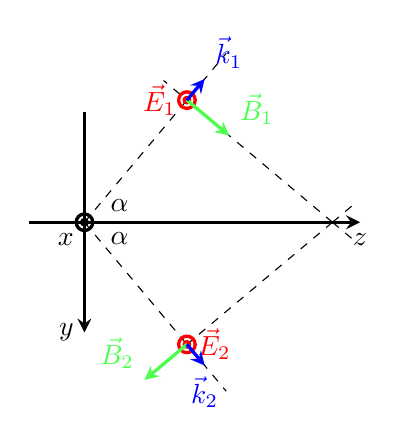
\begin{tikzpicture}[line width = 1.2pt, line join=round,>=stealth,scale=.7]
	\draw [->] (-1,0,0) -- (5,0,0) node[anchor=north] {$z$};
	\draw [->] (0,2,0) -- (0,-2,0) node[anchor=east] {$y$};
	\draw (0,0) circle (1.5 mm);
	\draw (0,0) circle (.5 mm) node[anchor=north east]{$x$};

	\draw[thin,dashed] (0,0) -- (50:4);
	\draw[thin,dashed] (0,0) -- (-50:4);

	\draw[thin,dashed] (4.5,0) -- +(140:4);
	\draw[thin,dashed] (4.5,0) -- +(-140:4);
	\draw[thin,dashed] (4.5,0) -- +(-40:.5);
	\draw[thin,dashed] (4.5,0) -- +(40:.5);

	\centerarc[thin,dotted](0,0)(0:50:1);
	\node at (25:0.7) {$\alpha$};
	\centerarc[thin,dotted](0,0)(0:-50:1);
	\node at (-25:0.7) {$\alpha$};

	\draw[red] (1.859,2.216) circle (1.5 mm);
	\draw[red] (1.859,2.216) circle (.5 mm) node[anchor=east]{$\vec{E}_1$};
	\draw[green!70, ->] (1.859,2.216) -- +(-40:1) node[anchor=south west]{$\vec{B}_1$};
	\draw[blue, ->] (1.859,2.216) -- +(50:.5) node[anchor=south west]{$\vec{k}_1$};

	\draw[red] (1.859,-2.216) circle (1.5 mm);
	\draw[red] (1.859,-2.216) circle (.5 mm) node[anchor=west]{$\vec{E}_2$};
	\draw[green!70, ->] (1.859,-2.216) -- +(-140:1) node[anchor=south east]{$\vec{B}_2$};
	\draw[blue, ->] (1.859,-2.216) -- +(-50:.5) node[anchor=north]{$\vec{k}_2$};

\end{tikzpicture}
		        \end{center}
		   \begin{align*}\ubar{\vec{E}}_1 = \ubar{\vec{E}}_0  \mathrm{e}^{\mathrm{j}(\omega t - \vec{k}_1\cdot\vec{r} )} = \ubar{E}_{0} \vu{x}  \mathrm{e}^{\mathrm{j}(\omega t - \vec{k}_1\cdot\vec{r} )} &\quad \text{ und }\quad
		         \vec{\ubar{B}}_1 = \dfrac{\vec{k}}{\omega}\times\ubar{\vec{E}}_1=\dfrac{1}{ v_\mathrm{p}} \left( \vu{{k_1}} \times \ubar{\vec{E}}_0  \mathrm{e}^{-\mathrm{j}\vec{k}_1\cdot\vec{r} }\right)  \mathrm{e}^{\mathrm{j}\omega t } \\
		  \ubar{\vec{E}}_2 = \ubar{\vec{E}}_0  \mathrm{e}^{\mathrm{j}(\omega t - \vec{k}_2\cdot\vec{r} )} = \ubar{E}_{0}\vu{x} \mathrm{e}^{\mathrm{j}(\omega t - \vec{k}_2\cdot\vec{r} )}&\quad \text{ und }\quad \vec{\ubar{B}}_2 = \dfrac{\vec{k}}{\omega}\times\ubar{\vec{E}}_2=\dfrac{1}{ v_\mathrm{p}} \left( \vu{{k_2}} \times \ubar{\vec{E}}_0  \mathrm{e}^{-\mathrm{j}\vec{k}_2\cdot\vec{r} }\right)  \mathrm{e}^{\mathrm{j}\omega t }\\
		  \vec{k}_1 = - k_y\vu{y} +  k_z\vu{z} & \quad \text{ und }\quad \vec{k}_2 =  k_y\vu{y} +  k_z\vu{z}  \end{align*}
		   \textbf{Überlagerung} der beiden Wellen:
		        \begin{equation*}\begin{split}
				        \ubar{\vec{E}} &= 2\ubar{E}_{0}\cos( k_yy) \vu{x}  \mathrm{e}^{\mathrm{j}(\omega t -  k_z z)} \\
				        \vec{\ubar{B}} &= \frac{2\ubar{E}_{0}}{ k  v_\mathrm{p}} \left(  k_z \cos( k_y y) \vu{y} + \mathrm{j} k_y\sin( k_y y) \vu{z}\right)  \mathrm{e}^{\mathrm{j}(\omega t -  k_z z)}
			        \end{split}\end{equation*}
		 $E$ ist transversal zur Ausbreitungsrichtung, $B$ hat auch eine longitudinale Komponente. Es handelt sich somit um eine \textbf{TE-Welle} (H-Welle), propagiert wird in $z$-Richtung. Ganz analog gibt es \textbf{TM-Wellen} (E-Wellen).\\
 Betrachtet man nun noch einmal die obige Grafik, dann stellt man fest, dass wenn $\alpha$ größer wird sich der Schnittpunkt der Wellenfronten immer schneller bewegen muss. Die Wellenfront bewegt sich entlang der Kathete, der Schnittpunkt entlang der Hypotenuse des rechtwinkligen Dreiecks. Für die Phasengeschwindigkeit folgt wegen der Ausbreitung in $z$-Richtung: \begin{equation*}
  	v_\mathrm{p} = \dfrac{\omega}{ k_z}
  \end{equation*}  
   Für die \textbf{einzelnen} Wellen gilt:
    \begin{equation*}
  v_\mathrm{c} = \dfrac{\omega}{ k} = \dfrac{\omega}{\sqrt{ k_y^2+ k_z^2}} \Rightarrow  k_z = \sqrt{\dfrac{\omega^2}{ v_\mathrm{c}^2}- k_y^2 }
  \end{equation*} 
		 Hiermit folgt für die Phasengeschwindigkeit:
		        \begin{equation*}\begin{split}
				        v_\mathrm{p} & = \frac{\omega}{ k_z} = \frac{\omega}{\sqrt{\frac{\omega^2}{ v_\mathrm{c}^2}- k_y^2 }} \\
				        & = \frac{\omega}{\frac{\omega}{ v_\mathrm{c}}\sqrt{1-\frac{ k_y^2  v_\mathrm{c}^2}{\omega^2} }} = \frac{ v_\mathrm{c}}{\sqrt{1-\frac{ k_y^2  v_\mathrm{c}^2}{\omega^2} }} \ge  v_\mathrm{c}
			        \end{split}\end{equation*}
		   Die Phasengeschwindigkeit ist hier also mindestens so groß wie die Ausbreitungsgeschwindigkeit im Medium (also insbesondere nicht gleich der Lichtgeschwindigkeit). Im Vakuum kann die Phasengeschwindigkeit somit \textbf{größer als die Lichtgeschwindigkeit} sein! Dass die Lichtgeschwindigkeit eine Obergrenze ist, gilt nur für Geschwindigkeiten, mit denen Information übertragen wird.
 \section{Allgemeine Lösung der homogenen Wellengleichung}
  \subsection{Darstellung als 4D-Fourier-Transformierte}
	  Es soll nun die \textbf{allgemeine Lösung} \(\Psi(\vec{r} ,t)\) der \textbf{homogenen Wellengleichung} ($\nearrow$\ref{homwell} mit \ref{geschwepsmu}) mit  vorgegebenen \textbf{Anfangswerten}
		        \begin{equation}\begin{split}
				        \Psi(\vec{r} ,t=0) &= \Psi_0(\vec{r} )\quad \text{ und}\\
				        \left.\frac{\partial \Psi(\vec{r} ,t)}{\partial t}\right|_{t=0} &= \dot{\Psi}_0(\vec{r} ) \quad\text{ betrachtet werden.}
			        \end{split}\end{equation}
		  Diese allgemeine Lösung lässt sich durch \textbf{Fourier-Transformation} ($\nearrow$\ref{fourtrans}) der partiellen Differentialgleichung finden. Die 4D-Fourier-Transformierte der noch unbekannten Lösung sei \(\tilde{\Psi}(\vec{k}, \omega)\) und existiert. Anzumerken ist, dass für viele zeitliche Abläufe die Fourier-Transformierte nicht existiert, weil das Integral nicht konvergiert. Bei Problemen, wo etwas abgestrahlt wird (also Antennen etc.) existiert die Fourier-Transformierte häufig schon. Deshalb wird \(\Psi(\vec{r} , t)\) formal als \textbf{Überlagerung ebener Wellen} mit beliebigen Wellenvektoren \(\vec{k}\) und Kreisfrequenzen \(\omega\) geschrieben:
		        \begin{equation}
			        \Psi(\vec{r} , t) = \frac{1}{(2\pi)^4} \iiint\limits_{\mathbb{R}^3} \int\limits_{-\infty}^\infty \tilde{\Psi}(\vec{k}, \omega)  \mathrm{e}^{\mathrm{j}(\vec{k}\cdot\vec{r} -\omega t)} \dd \omega \dd^3k
		        \end{equation}
		   Dass $\vec{k}\cdot\vec{r}$ und $\omega t$ gegensätzliche Vorzeichen haben, ist Konvention. $\omega$ kann hier auch negativ sein (zweiseitiges Spektrum einfacher zu rechnen). Wegen der Überlagerung zu beliebigen Ausbreitungsrichtungen ist die Lösung im Allgemeinen \textbf{keine ebene Welle} (nicht zwangsläufig TEM-Welle).	 Die Schreibweise als 4-dimensionale Fouriertransformierte erlaubt es, die Ableitungen explizit auszuführen:
		        \begin{equation}
			        \Delta  \mathrm{e}^{\mathrm{j}(\vec{k}\cdot\vec{r} -\omega t)} = -k^2  \mathrm{e}^{\mathrm{j}(\vec{k}\cdot\vec{r} -\omega t)}\quad \text{ und }\quad \frac{\partial^2}{\partial t^2} \mathrm{e}^{\mathrm{j}(\vec{k}\cdot\vec{r} -\omega t)}= -\omega^2 \mathrm{e}^{\mathrm{j}(\vec{k}\cdot\vec{r} -\omega t)}
		        \end{equation}
		 Die homogene Wellengleichung ($\nearrow$\ref{homwell}) schreibt sich damit in der Form
		        \begin{equation}
			        \frac{1}{(2\pi)^4} \iiint\limits_{\mathbb{R}^3} \int\limits_{-\infty}^\infty \left(-k^2+\frac{\omega^2}{ v_\mathrm{c}^2} \right)\tilde{\Psi}(\vec{k}, \omega)  \mathrm{e}^{\mathrm{j}(\vec{k}\cdot\vec{r} -\omega t)} \dd \omega \dd^3k  = 0
		        \end{equation}
		  Dies kann aber allgemein nur erfüllt werden, wenn gilt
		        \begin{equation}
			        \boxed{\left(\frac{\omega^2}{ v_\mathrm{c}^2} -k^2 \right)\tilde{\Psi}(\vec{k}, \omega)  = 0}
		        \end{equation}
		  Durch den Übergang zur Fourier-Transformierten resultiert eine zur homogenen Wellengleichung \textbf{äquivalente algebraische Gleichung}. Die triviale Lösung $\tilde{\Psi}(\vec{k}, \omega)=0$ ist nicht von Interesse. Deshalb ist die bereits vorher bei ebenen Wellen und Kugelwellen gefundene Beziehung
		        \begin{equation}\label{omkv}
			        \boxed{\omega = \pm  v_\mathrm{c} k}
		        \end{equation}
		        eine allgemeingültige Beziehung im Kontext der homogenen Wellengleichung.
  \subsection{Darstellung als 3D-Fourier-Transformierte}
   Den bisher eingeschlagenen Weg über eine 4D-Transformierte könnte man problemlos weitergehen und würde eine allgemeine Lösung der Wellengleichung zu den Anfangswerten finden. Um eine bestimmte Formulierung, die Kirchhoffsche Lösung, zu finden, wird der Ansatz variiert. Die Erkenntnis \ref{omkv} wird aber weiter genutzt. Man setzt nun eine 3D-Fourier-Transformierte an (beachte: $\omega$ und $k$ sind voneinander abhängig!): 
		        \begin{align}
			        \tilde{\Psi}(\vec{k}, \textcolor{red}{t}) & = \iiint\limits_{\mathbb{R}^3} \Psi (\vec{r} , \textcolor{red}{t})  \mathrm{e}^{-\mathrm{j}\vec{k}\cdot\vec{r} } \dd^3 r                         &  & \text{ Hintransformation}  \\
			        \Psi(\vec{r} , \textcolor{red}{t})        & = \frac{1}{(2\pi)^3}\iiint\limits_{\mathbb{R}^3} \tilde{\Psi} (\vec{k}, \textcolor{red}{t})  \mathrm{e}^{\mathrm{j}\vec{k}\cdot\vec{r} } \dd^3 k &  & \text{ Rücktransformation}
		        \end{align}
		  Transformation der Anfangswerte liefert:
		        \begin{equation}
			        \tilde{\Psi}_0(\vec{k}) = \iiint\limits_{\mathbb{R}^3} \Psi_0 (\vec{r} )  \mathrm{e}^{-\mathrm{j}\vec{k}\cdot\vec{r} } \dd^3 r \quad\text{ und }\quad
			        \tilde{\dot{\Psi}}_0(\vec{k}) = \iiint\limits_{\mathbb{R}^3} \dot{\Psi}_0 (\vec{r} )  \mathrm{e}^{-\mathrm{j}\vec{k}\cdot\vec{r} } \dd^3 r
		        \end{equation}
  \subsection{Kirchhoffsche Lösung}\label{kirchlsg}
		  Einsetzen in die homogene Wellengleichung ($\nearrow$\ref{homwell}) ergibt:
		        \begin{equation}
			        \frac{1}{(2\pi)^3}\iiint\limits_{\mathbb{R}^3} \left(-k^2 -\frac{1}{ v_\mathrm{c}^2}\frac{\partial^2}{\partial t^2}\right)\tilde{\Psi} (\vec{k}, t)  \mathrm{e}^{\mathrm{j}\vec{k}\cdot\vec{r} } \dd^3 k = 0
		        \end{equation}
		  Dies führt auf ein einfaches Anfangswertproblem für \(\tilde{\Psi} (\vec{k}, t)\):
		        \begin{equation}
			        \left(\frac{1}{ v_\mathrm{c}^2}\frac{\partial^2}{\partial t^2} + k^2 \right)\tilde{\Psi} (\vec{k}, t) =0 ; \quad \tilde{\Psi}(\vec{k}, 0) = \tilde{\Psi}_0(\vec{k}), \quad \tilde{\dot{\Psi}}(\vec{k}, 0) = \tilde{\dot{\Psi}}_0(\vec{k})
		        \end{equation}
		  Die allgemeine Lösung für dieses Problem lautet (Zusammenhang \ref{omkv} nun genutzt): 
		  \begin{equation}
		  	\boxed{\tilde{\Psi} (\vec{k}, t) = A(\vec{k}) \cos( k v_\mathrm{c}t) + B(\vec{k}) \sin( k v_\mathrm{c}t)}
		  \end{equation}
		  Für die Konstanten folgt: 
		  \begin{equation}\begin{split} \tilde{\Psi}(\vec{k}, 0) = \Aboxed{\tilde{\Psi}_0(\vec{k}) &= A(\vec{k})} \\
		       \left. \frac{\partial}{\partial t} \tilde{\Psi}(\vec{k}, t)\right|_{t=0}  =  k v_\mathrm{c} B(\vec{k}) = \tilde{\dot{\Psi}}_0(\vec{k}) \to \Aboxed{B(\vec{k}) &= \frac{\tilde{\dot{\Psi}}_0(\vec{k})}{ k v_\mathrm{c}}}\end{split}\end{equation}
	       Durch die Anfangswerte ist die Fouriertransformierte nun komplett bekannt. Einsetzen in die Rücktransformation ergibt die \textbf{allgemeine Lösung der homogenen Wellengleichung} mit \textbf{Anfangswerten}:
		        \begin{align}\label{allglsganf}
			        \Aboxed{\Psi(\vec{r} , t) & = \frac{1}{(2\pi)^3}\iiint\limits_{\mathbb{R}^3} \left[ \tilde{\Psi}_0(\vec{k}) \cos( k v_\mathrm{c}t) + \tilde{\dot{\Psi}}_0(\vec{k}) \frac{\sin( k v_\mathrm{c}t)}{ k v_\mathrm{c}} \right] \mathrm{e}^{\mathrm{j}\vec{k}\cdot\vec{r} } \dd^3 k \text{ mit}}                            \\
			        \tilde{\Psi}_0(\vec{k})   & = \iiint\limits_{\mathbb{R}^3} \Psi_0 (\vec{r} )  \mathrm{e}^{-\mathrm{j}\vec{k}\cdot\vec{r} } \dd^3 r \quad \text{ und } \quad\tilde{\dot{\Psi}}_0(\vec{k}) = \iiint\limits_{\mathbb{R}^3} \dot{\Psi}_0 (\vec{r} )  \mathrm{e}^{-\mathrm{j}\vec{k}\cdot\vec{r} } \dd^3 r \nonumber
		        \end{align}
		   Diese allgemeine Lösung kann noch etwas umgeschrieben werden, um Eigenschaften leichter ablesen zu können. Offenbar gilt: \begin{equation}\cos( k v_\mathrm{c}t)  = \frac{\partial}{\partial t}\left( \frac{\sin( k v_\mathrm{c}t)}{ k v_\mathrm{c}} \right)\end{equation}
		   Außerdem kann \textbf{\(R(t) =  v_\mathrm{c}t \)} interpretiert werden als den \textbf{Weg, den eine einzelne Wellenfront seit \(t=0\) zurückgelegt hat}. Es kann ersetzt werden: \(  v_\mathrm{c} = \frac{R(t)}{t}\).
		   Weiterhin gilt folgende Identität (\(K_R\): Kugel im Ursprung mit Radius $R$):
		        \begin{equation}
			        \frac{\sin  k R}{ k R} = \frac{1}{4\pi R^2} \oiint\limits_{O(K_R)}  \mathrm{e}^{\mathrm{j}\vec{k} \cdot \vec{r} '} \dd^2 r' = \frac{1}{4\pi R^2} \int\limits_0^{2\pi}\int\limits_0^\pi  \mathrm{e}^{\mathrm{j}\vec{k} \cdot \vec{r} '} R^2\sin\vartheta\dd\vartheta\dd\varphi
		        \end{equation}
		   Einsetzen der Beziehungen liefert unter Vertauschung der Integrationsreihenfolge: 
		        \begin{equation}\begin{split}
				        \Psi(\vec{r} , t) = \frac{\partial}{\partial t} &\left[ \frac{t}{4\pi R^2} \oiint\limits_{O(K_R)} \left\{ \frac{1}{(2\pi)^3}\iiint\limits_{\mathbb{R}^3}  \tilde{\Psi}_0(\vec{k})  \mathrm{e}^{\mathrm{j}\vec{k} \cdot (\vec{r} +\vec{r} ')} \dd^3 k\right\} \dd^2 r' \right] \\
				        + &\left[ \frac{t}{4\pi R^2} \oiint\limits_{O(K_R)} \left\{ \frac{1}{(2\pi)^3}\iiint\limits_{\mathbb{R}^3}  \tilde{\dot{\Psi}}_0(\vec{k})  \mathrm{e}^{\mathrm{j}\vec{k} \cdot (\vec{r} +\vec{r} ')} \dd^3 k\right\} \dd^2 r' \right]
			        \end{split}\end{equation}
Vereinfachen des Ganzen liefert die \textbf{Kirchhoffsche Lösung} als allgemeine Lösung der homogenen Wellengleichung mit Anfangswerten:
		        \begin{equation}
			        \boxed{\Psi(\vec{r} , t) = \frac{\partial}{\partial t} \left[ \frac{t}{4\pi R^2(t)} \oiint\limits_{O(K_{R(t)})} \Psi_0(\vec{r} +\vec{r} ') \dd^2 r' \right]
				        + \left[ \frac{t}{4\pi R^2(t)} \oiint\limits_{O(K_{R(t)})} \dot{\Psi}_0(\vec{r} +\vec{r} ') \dd^2 r' \right]}
		        \end{equation}
		        Die eindimensionale Formulierung dieser Gleichung heißt d'Alembertsche Lösung und kann \href{https://de.wikipedia.org/wiki/Wellengleichung#Die_Wellengleichung_in_einer_r%C3%A4umlichen_Dimension}{direkt} oder über die 1D-Betrachtung von \ref{allglsganf} gewonnen werden:
		        \begin{equation}
		        	\begin{split}
		        		\Psi(z , t) & = \frac{1}{(2\pi)}\int\limits_{\IR} \left[ \tilde{\Psi}_0(k)  \cos( k v_\mathrm{c}t) + \tilde{\dot{\Psi}}_0(k) \frac{\sin( k v_\mathrm{c}t)}{ k v_\mathrm{c}} \right] \mathrm{e}^{\mathrm{j}kz } \dd k\\
		        		&=\underbrace{\mathcal{F}^{-1}\left\{ \tilde{{\Psi}}_0(k)\right\} * \mathcal{F}^{-1}\left\{ \frac{\mathrm{e}^{\mathrm{j}kv_\mathrm{c}t}+\mathrm{e}^{-\mathrm{j}kv_\mathrm{c}t}}{2}\right\}}_{\text{Faltungssatz der Fouriertransformation}}\\
		        		&\phantom{=}+\frac{1}{2\pi}\iint\limits_{\IR^2} \dot{\Psi}_0(z')\mathrm{e}^{-\mathrm{j}kz'} \dd z' \underbrace{\frac{\mathrm{e}^{\mathrm{j}kv_\mathrm{c}t}-\mathrm{e}^{-\mathrm{j}kv_\mathrm{c}t}}{2\mathrm{j}kv_\mathrm{c}}\mathrm{e}^{\mathrm{j}kz}}_{\frac{1}{2v_\mathrm{c}}\int\limits_{z-v_\mathrm{c}t}^{z+v_\mathrm{c}t}\mathrm{e}^{\mathrm{j}ku} \dd u} \dd k\\
		        		&=\frac{1}{2}\Psi_0(z-v_\mathrm{c}t)+\frac{1}{2}\Psi_0(z+v_\mathrm{c}t)+\frac{1}{2v_\mathrm{c}}\int\limits_{z-v_\mathrm{c}t}^{z+v_\mathrm{c}t} \underbrace{\frac{1}{2\pi}\iint\limits_{\IR^2} \dot{\Psi}_0(z')\mathrm{e}^{\mathrm{j}k(u-z')}\dd k \dd z'}_{\stackrel{\nearrow\text{\ref{diracft}}}{=}\dot{\Psi}_0(u)} \dd u \\
		        	\Aboxed{	\Psi(z , t)&=\frac{1}{2}\Psi_0(z-v_\mathrm{c}t)+\frac{1}{2}\Psi_0(z+v_\mathrm{c}t)+\frac{1}{2v_\mathrm{c}}\int\limits_{z-v_\mathrm{c}t}^{z+v_\mathrm{c}t} \dot{\Psi}_0(u) \dd u}
		        	\end{split}
		        \end{equation}
  \subsection{Interpretation - Huygens-Fresnelsches Prinzip}\label{huy}
  Zum Zeitpunkt $t_1$ wird die Welle am Ort $\vec{r}$ durch die Anfangswerte auf der blauen Kugel bestimmt. Zu einem späteren Zeitpunkt $t_2$ wäre der Radius $R$ der Kugel größer. Die grünen Kugeln zeigen jeweils, an welchen Orten der Anfangswert vom Mittelpunkt der Kugel zum Zeitpunkt $t_1$ einen Einfluss hat. Die Superposition der Wirkungen aller Elementarwellen (also aller grünen Kreise) im Punkt $\vec{r}$ führt auf die Welle in diesem Punkt.
	  \begin{center}
		  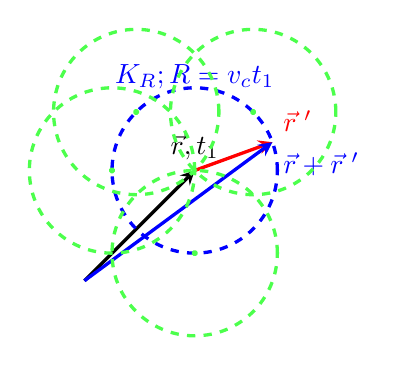
\begin{tikzpicture}[line width = 1.2pt, line join=round,>=stealth, scale=0.7]
	\draw [->,   ] (-2,-2) -- (0,0) node[anchor=south,   ] {$\vec{r} , t_1$};
	\draw [red,->,   ] (0,0) -- (20:1.5) node[anchor=south west,   ] {$\vec{r} \;'$};
	\draw [blue,->,   ] (-2,-2) -- (20:1.5) node[anchor=north west,   ] {$\vec{r} +\vec{r} \;'$};

	\draw[blue, dashed,   ] (0,0) circle (1.5);
	{\node[blue] at (0,1.7) {$K_R; R=v_ct_1$};}

	\draw[green!70,   ] (45:1.5) circle (0.03);
	\draw[green!70, dashed,   ] (45:1.5) circle (1.5);

	\draw[green!70,   ] (135:1.5) circle (0.03);
	\draw[green!70, dashed,   ] (135:1.5) circle (1.5);

	\draw[green!70,   ] (180:1.5) circle (0.03);
	\draw[green!70, dashed,   ] (180:1.5) circle (1.5);

	\draw[green!70,   ] (270:1.5) circle (0.03);
	\draw[green!70, dashed,   ] (270:1.5) circle (1.5);

\end{tikzpicture}
	  \end{center}
	  Jeder Punkt einer Wellenfront ist Ausgangspunkt einer neuen Welle (also eine Anfangsbedingung), der so genannten \textbf{Elementarwelle}. Die Elementarwelle hat die gleiche Frequenz und Ausbreitungsgeschwindigkeit wie die Primärwelle. Die neue Wellenfront ergibt sich durch phasenrichtige Addition -- \textbf{Superposition} -- sämtlicher Elementarwellen. Im dreidimensionalen Raum breiten sich die Elementarwellen \textbf{kugelförmig} aus. Das heißt, dass eine Anregung an einem Punkt nach einer gewissen Zeit ihre Wirkung an allen Punkten einer Kugeloberfläche entfaltet. Phasenfronten entsprechen also einer Kugel. Das ist nicht zu verwechseln mit der kugelsymmetrischen Lösung der Wellengleichung, welche einen inhärenten Widerspruch darstellt ($\nearrow$\ref{kugwell}). Dort war kritisch, dass $\Psi(\vec{r},t)=\Psi(r,t)$ golt, die Komponenten der Vektoren also keine $\varphi$ oder $\vartheta$-Abhängigkeit haben durften. Diese Einschränkung gilt für allgemeine Wellen nicht.
\subsection{Konzeptionelle Zusammenfassung - Superposition}
Insbesondere werden im gesamten Kapitel zu den elektromagnetischen Wellen die (1) monochromatischen (2) ebenen Wellen (3) linearer Polarisation betrachtet. Dabei können ebene Wellen als solche praktisch gar nicht auftreten, es wäre eine unendliche ausgedehnte Wellenfront und damit auch unendlich viel Energie nötig. Es stellt sich also die Frage, warum den praktisch unmöglichen Wellen hier so viel Platz eingeräumt wird.\\
Die \textbf{Maxwell-Gleichungen} sind \textbf{lineare} pDGLs. Das heißt insbesondere, dass \textbf{Superpositionen} möglich sind.
\begin{enumerate}
	\item Man kann im Sinne einer klassischen Fourier-Synthese \textbf{monochromatische} Wellen verschiedener Frequenzen überlagern und erhält so die allgemeinere \textbf{polychromatische} Wellen (bspw. eine Dreieckspannung auf einem Leiter) ($\nearrow$\ref{fourtrans}).
	\item Das Selbe kann man mit einer \textbf{3D-Fourier-Transformierten} im $k$-Raum machen, d.h. man kann verschiedene Wellenvektoren (wie Frequenzen) superponieren und erhält so allgemeinere Wellenformen ($\nearrow$\ref{fourtrans}).
	\item Es ist zudem möglich aus zwei \textbf{senkrecht} zueinander stehenden \textbf{linearen Polarisationen} eine \textbf{beliebige Polarisation} zu konstituieren ($\nearrow$\ref{poleb}).
\end{enumerate}
Dies ist konzeptionell dem Huygens-Fresnelschen Prinzip sehr ähnlich (Superposition von Elementarwellen). 
 \section{Ebene Wellen als Lösung der Telegraphen-Gleichung (leitende Medien)}\label{leitendeMed}
 Bisher wurde sowohl die Ladungsträgerdichte \(\rho_\text{V}\) als auch die Stromdichte \(\vec{J}\) als identisch Null angenommen ($\nearrow$\ref{annhomwell}). Dies entspricht der \textbf{Ausbreitung in isolierenden Dielektrika} und ohne weitere Quellen. Für die \textbf{Anwendung wichtig} sind aber auch \textbf{Wellenausbreitungen in leitfähigen (verlustbehafteten) Medien}. In diesem Fall sind das elektrische Feld \(\vec{E}\) und die (Leitungs-) Stromdichte \(\vec{J}\) entsprechend \ref{ohm} über die elektrische Leitfähigkeit \(\kappa\) miteinander verknüpft. Weiter sollen neutrale, also \(\rho_\text{V} = 0\), sowie homogene, isotrope und lineare Medien angenommen werden.
   \subsection{Telegraphen-Gleichungen}
    Die Annahmen lauten zusammengefasst im Gegensatz zu \ref{annhomwell}:
 \begin{equation}\label{anntelegraph}
 	\text{hli, }\quad\rho_\text{V}=0 \quad \text{ und }\quad\vec{J}=\kappa\vec{E}.
 \end{equation}
 Die Maxwell Gleichungen ($\nearrow$\ref{ind},\ref{quellf},\ref{durchf},\ref{gauss}) lauten unter diesen Annahmen:
		        \begin{align}
			        \rot \vec{E} & = -\frac{\partial \vec{B} }{\partial t} & \div \vec{E} & = 0 & \rot \vec{B} & = \mu\kappa \vec{E} + \mu\varepsilon \frac{\partial \vec{E}}{\partial t} & \div \vec{B} & = 0
		        \end{align}
		  Diese Gleichungen können wieder wie üblich über \ref{rotrot} entkoppelt werden. Die entkoppelten Maxwellgleichungen sind die \textbf{Telegraphen-Gleichungen}, die für \(\kappa \to 0\) in die Wellengleichungen übergehen:
		        \begin{equation}\begin{split}
				        \Aboxed{\left[\Delta - \varepsilon\mu \frac{\partial^2}{\partial t^2} -\mu\kappa \frac{\partial}{\partial t}\right]\vec{E}(\vec{r} , t) = \left[\square -\mu\kappa \frac{\partial}{\partial t}\right]\vec{E}(\vec{r} , t) &= \vec{0}}\\
				        \Aboxed{\left[\Delta - \varepsilon\mu \frac{\partial^2}{\partial t^2} -\mu\kappa \frac{\partial}{\partial t}\right]\vec{B} (\vec{r} , t) = \left[\square -\mu\kappa \frac{\partial}{\partial t}\right]\vec{B} (\vec{r} , t)&= \vec{0}}
			        \end{split}\end{equation}
		  Der Wellenoperator wird also durch einen zusätzlichen Term modifiziert. Wie schon im Falle der homogenen Wellengleichung kann sich für die Analyse auf eine Feldkomponente beschränkt werden, die wieder als \(\Psi(\vec{r} , t)\) bezeichnet wird. Es soll der wichtige Spezialfall \textbf{harmonischer Zeitabhängigkeit} betrachtet werden, wobei der Hinweis zur Normierung aus \ref{harmebwell} zu beachten ist:
		        \begin{align}
			        \Psi(\vec{r} , t) & = \re{\underline{\Psi}(\vec{r} , t)} & \underline{\Psi}(\vec{r} , t) & = \underline{\Psi}_0(\vec{r} )  \mathrm{e}^{\mathrm{j}\omega t} & \frac{\partial}{\partial t} \underline{\Psi} & = \mathrm{j}\omega \underline{\Psi} & \frac{\partial^2}{\partial t^2} \underline{\Psi} & = -\omega^2 \underline{\Psi}
		        \end{align}
		   Die Telegraphen-Gleichung lautet dann:
		        \begin{equation}
			        \boxed{\left[ \Delta + \omega^2\varepsilon\mu - \mathrm{j}\omega\mu\kappa \right] \underline{\Psi}(\vec{r} , t) =0}
		        \end{equation}
  \subsection{Lösung der Telegraphen-Gleichung mit komplexen Größen}
  \subsubsection{Abgrenzung: Komplexe Permittivität im Dielektrikum}
  Im Gegensatz zum Vakuum ist das Verhalten beim Anlegen eines Wechselfeldes in Materialien frequenzabhängig. Es kommt auch zu einer Phasenverschiebung des elektrischen Feldes gegenüber der elektrischen Flussdichte, da sich die atomaren Strukturen nicht instantan umpolarisieren. Man definiert:
  \begin{equation}\label{komplperm1}
  	\boxed{\ubar{\varepsilon}(\omega)=\varepsilon'(\omega)+\mathrm{j}\varepsilon''(\omega)
  	=|\ubar{\varepsilon}(\omega)|(1-\mathrm{j}\tan\delta)=\frac{\ubar{D}}{\ubar{E}}}
  \end{equation}
 Es gibt unterschiedliche Konventionen bei dieser Definition. $\delta$ ist der sogenannte \textbf{Verlustwinkel}. Der Imaginärteil sorgt also für Verluste, anschaulich sind das Reibungsverluste durch die Schwingung (harmonischer Oszillator $\to$ Term, der proportional zur zeitlichen Ableitung ist führt zu Verlusten wie beim Federpendel). Insbesondere ist die komplexe Permittivität wegen atomarer Effekte frequenzabhängig (\href{https://de.wikipedia.org/wiki/Datei:Dielectric_responses.svg}{Bildquelle}):\\
 \begin{minipage}{0.39\textwidth}
 	\includegraphics[width=0.9\textwidth]{res/Dielectric_responses_DE.pdf}
 \end{minipage}\hfill
 \begin{minipage}{0.6\textwidth}
 	Grundsätzlich gibt es beim Anlegen eines zeitlich veränderlichen Feldes ein verschiedenes Verhalten bei vorhandenen oder nicht
 	vorhandenen Rückstellkräften. \textbf{Dipolar} orientieren sich polare Moleküle (z.B.
 	Wasser) im Feld, es gibt keine Rückstellkraft, nur thermische Bewegung (Debye-Relaxation).
 	\textbf{Molekular} und \textbf{atomar} (kleinere Größe $\to$ höhere Frequenz, wo der Effekt zum Tragen kommt) sind Rückstellkräfte vorhanden (harmonischer Oszillator, Schwingkreis $\to$ Kurve sieht so aus wie Impedanzverlauf im Schwingkreis).
 	Die dielektrische Spektroskopie dient zur Aufklärung der Mechanismen.
 \end{minipage}\\\\
 Dieser Abschnitt diente zur Abgrenzung, denn bei der Lösung der Telegraphen-Gleichung wird auch eine komplexe Permittivität eingeführt, die aber nicht mit den hier beschriebenen molekularen Effekten zusammenhängt.
 \subsubsection{Eigentliche Lösung der Telegraphen-Gleichung}
		  Die Telegraphen-Gleichung bei harmonischer Zeitabhängigkeit kann leicht in die bekannte Form der homogenen \textbf{Wellengleichung} ($\nearrow$\ref{homwell}) überführt werden:
		        \begin{equation}\begin{split}
				        \left[ \Delta + \omega^2\varepsilon\mu - \mathrm{j}\omega\mu\kappa \right] \underline{\Psi}(\vec{r} , t) =\left[ \Delta + \omega^2\mu\left(\varepsilon - \mathrm{j}\frac{\kappa}{\omega}\right) \right] \underline{\Psi}(\vec{r} , t) &=0\\
				        \left[ \Delta + \omega^2\mu_0\mu_r\varepsilon_0\left(\varepsilon_r - \mathrm{j}\frac{\kappa}{\varepsilon_0\omega}\right) \right] \underline{\Psi}(\vec{r} , t) &=0\\
				        \left[ \Delta + \frac{\omega^2}{c^2}\underline{\varepsilon}_r\mu_r\right] \underline{\Psi}(\vec{r} , t) = \left[ \Delta + \frac{\omega^2}{ \ubar{v}_\mathrm{c}^2}\right] \underline{\Psi}(\vec{r} , t)&=0
			        \end{split}\end{equation}
		 Hierbei wurde eine \textbf{komplexe Permittivität} \(\underline{\varepsilon}_r\) eingeführt ($\nearrow$\ref{komplperm1}):
		        \begin{equation}\begin{split}
			        \Aboxed{\underline{\varepsilon}_r &= \varepsilon_r^{\prime} + \mathrm{j}\varepsilon_r^{\prime\prime} = \varepsilon_r - \mathrm{j}\frac{\kappa}{\varepsilon_0\omega} = |\underline{\varepsilon}_r|  \mathrm{e}^{-\mathrm{j}\delta}} \\ |\underline{\varepsilon}_r|&=\sqrt{\varepsilon_r^2+\frac{\kappa^2}{\varepsilon_0^2\omega^2}} \\
			        \tan\delta &= \frac{\kappa}{\varepsilon_0\varepsilon_r\omega} \\
			        \underline{\varepsilon}_r &=\varepsilon_r (1 - \mathrm{j}\tan\delta)
		        \end{split}\end{equation}
		        Man sollte beachten, dass hier von einer \textbf{reellen Permittivität} ausgegangen wurde und dann ein Term mit der Leitfähigkeit in die Permittivität hineindefiniert wurde. Genauso kann man hier auch von einer \textbf{komplexen Permittivität} ausgehen (die wie im Abschnitt zuvor den molekularen Effekten Rechnung trägt). Das führt dann dazu, dass der Imaginärteil zwei Komponenten hat. Welche Terme man betrachtet und welche man (näherungsweise) vernachlässigt, ist vom jeweiligen Problem abhängig (im guten Leiter dominiert häufig der Imaginärteil, in einem guten Dielektrikum häufig der Realteil). Jede komplexe Permittivität führt zu Verlusten, weshalb $\delta$ auch Verlustwinkel heißt.\\
		   Außerdem ergibt sich die \textbf{komplexe Ausbreitungsgeschwindigkeit} \( \ubar{v}_\mathrm{c}\):
		        \begin{equation}
			        \boxed{ \ubar{v}_\mathrm{c} = \frac{1}{\sqrt{\varepsilon_0\underline{\varepsilon}_r\mu_0\mu_r}} = \frac{1}{\sqrt{\underline{\varepsilon}\mu}}}
		        \end{equation}
		 Aus den Betrachtungen zur Wellengleichung in \ref{harmebwell} folgt vollkommen analog (nur hier mit einem komplexen Wellenvektor) die Lösung der Telegraphengleichung:
		        \begin{equation}
			        \boxed{\underline{\Psi}(\vec{r} , t) = \underline{\Psi}_0  \mathrm{e}^{\mathrm{j}(\omega t -  \vec{\ubar{k}}\cdot\vec{r} )}}
		        \end{equation}
		 Hierbei ist \( \vec{\ubar{k}}\) der \textbf{komplexe Wellenvektor}, der sich aus der komplexen Ausbreitungsgeschwindigkeit ergibt:
		        \begin{equation}
			        \vec{\ubar{k}} = \frac{\omega}{ \ubar{v}_\mathrm{c}} \vu{k} = \omega \sqrt{\underline{\varepsilon}\mu}\, \vu{k}= \frac{\omega}{c} \sqrt{\underline{\varepsilon}_r\mu_r}\, \vu{k} = \frac{\omega}{c} \underline{n}\, \vu{k}
		        \end{equation}
		  Außerdem wurde der \textbf{komplexe Brechungsindex} \(\underline{n}\) eingeführt, dessen Realteil $n^{\prime}$ auch \textbf{verallgemeinerter Brechungsindex} und dessen Imaginärteil $\gamma$ auch \textbf{Extinktionskoeffizient} genannt wird:
		        \begin{equation}\begin{split}
				        \underline{n} &= \sqrt{\underline{\varepsilon}_r\mu_r} = n^{\prime} - \mathrm{j}\gamma \text{ mit}\\
				        n^{\prime} &= n\cdot \sqrt{ \frac{1}{2}+\frac{1}{2}\sqrt{1+ \left( \frac{\kappa}{\varepsilon_0\varepsilon_r\omega} \right)^2} } \xrightarrow{\kappa\to 0} n \\
				        \gamma &= n \cdot \sqrt{-\frac{1}{2}+\frac{1}{2}\sqrt{1+ \left( \frac{\kappa}{\varepsilon_0\varepsilon_r\omega} \right)^2} } \xrightarrow{\kappa\to 0} 0 
			        \end{split}\end{equation}
  \subsection{Lösung für die Felder}
		 Setzt man die gefundene Lösung z.B. für das elektrische Feld ein ergibt sich:
		        \begin{equation}\begin{split}
				        \ubar{\vec{E}}(\vec{r} , t) &= \ubar{\vec{E}}_0  \mathrm{e}^{\mathrm{j}(\omega t -  \vec{\ubar{k}}\cdot\vec{r} )}\\
				        &=\ubar{\vec{E}}_0  \mathrm{e}^{\mathrm{j}(\omega t - \frac{\omega}{c}\underline{n}\vu{k}\cdot\vec{r} )} = \ubar{\vec{E}}_0  \mathrm{e}^{\mathrm{j}(\omega t - \frac{\omega}{c}(n^{\prime}-\mathrm{j}\gamma)\vu{k}\cdot\vec{r} )}\\
				        &= \ubar{\vec{E}}_0 \mathrm{e}^{-\frac{\omega}{c}\gamma \vu{k}\cdot\vec{r} }  \mathrm{e}^{\mathrm{j}(\omega t - \frac{\omega}{c}n^{\prime}\vu{k}\cdot\vec{r} )} = \ubar{\vec{E}}_0 \mathrm{e}^{- k^{\prime\prime} \vu{k}\cdot\vec{r} }  \mathrm{e}^{\mathrm{j}(\omega t -  k^{\prime}\vu{k}\cdot\vec{r} )}
			        \end{split}\end{equation}
		  Dies beschreibt eine \textbf{gedämpfte Welle} in Richtung \(\vu{k} \) mit \textbf{Eindringtiefe} \(\delta = \frac{c}{\omega\gamma}\). Je größer also der Extinktionskoeffizient (je größer also die Leitfähigkeit), desto weniger stark dringt die Welle in das Medium ein. Die \textbf{Phasengeschwindigkeit} ließt man aus dem Wellenterm ab:
		        \begin{equation}
			        \boxed{ v_\mathrm{p} = \frac{\omega}{ k^{\prime}} = \frac{c}{n^{\prime}} \le \frac{c}{n}} 
		        \end{equation}
		   Diese ist offensichtlich maximal für $\kappa=0$. Für die magnetische Flussdichte gilt:
		        \begin{equation}
			        \vec{\ubar{B}}(\vec{r} , t) = \vec{\ubar{B}}_0  \mathrm{e}^{\mathrm{j}(\omega t -  \vec{\ubar{k}}\cdot\vec{r} )}
		        \end{equation}
		        folgt analog zu den früheren Herleitungen:
		        \begin{equation}
			        \vec{\ubar{k}}\cdot\ubar{\vec{E}} = 0 \; ,\quad  \vec{\ubar{k}}\cdot\vec{\ubar{B}} = 0 \; ,\quad \frac{ \ubar{k}}{\omega} \vu{k}\times \ubar{\vec{E}} = \boxed{\vec{\ubar{B}} = \frac{1}{c}(n^{\prime}-\mathrm{j}\gamma) \vu{k}\times \ubar{\vec{E}}}
		        \end{equation}
		        Es handelt sich also um eine \textbf{TEM-Welle}, $E$ und $B$ sind aber \textbf{nicht in Phase}.

 \section{Reflexion und Brechung von ebenen Wellen}
 Das Medium, aus dem die Welle einfällt, heißt Medium 1. Entsprechend ist das andere Medium 2 und der Normalenvektor ist von 1 nach 2 orientiert. Die geometrischen Größen und Materialparameter sind wie in der folgenden Grafik definiert. In der Grafik ist zudem verdeutlicht, dass zunächst noch unbekannt ist, ob die Wellenvektoren von reflektierter und transmittierter Welle in der Einfallsebene liegen.\\
  \begin{minipage}{.5\textwidth}
	  \resizebox*{\textwidth}{!}{\tdplotsetmaincoords{70}{20}
\begin{tikzpicture}[scale=0.6,tdplot_main_coords]
	\draw[fill=gray!50,canvas is xy plane at z=0] (-5,-5) rectangle (5,5);
	\node[transform shape,canvas is xy plane at z=0,anchor=south west]
	at (-5,-5) {{\huge Grenzfläche}};
	\draw[-stealth] (-5.5,0,0) -- (5.5,0,0) node[pos=1.05]{$x$};
	\draw[-stealth] (0,5.5,0) -- (0,-5.5,0) node[pos=1.05]{$y$};
	\draw[-stealth] (0,0,5) -- (0,0,-2.5) node[pos=1.025]{$z$};
	\begin{scope}[canvas is xy plane at z=0]
		\draw[-latex] (2.5,0) arc(0:-40:2.5) node[below right]{$\varphi_r, \; \varphi_t$};
	\end{scope}

	\foreach \X [count=\Y,evaluate=\Y as \Col using {int(\Y*20)}] in {0,-20,-40}
		{\tdplotsetrotatedcoords{\X}{00}{0}
			\begin{scope}[tdplot_rotated_coords]
				\begin{scope}[canvas is xz plane at y=0]
					\draw[fill=blue!\Col, fill opacity=0.5] (0:2.5) arc (0:90:2.5) -- (0,0);
				\end{scope}
			\end{scope}}

	\begin{scope}[canvas is xz plane at y=0]
		\draw[fill=blue!20,fill opacity=0.5] (90:4.2) arc (90:180:4.2) -- (0,0);
		\draw[thick] (150:6.5) node[above,align=center]{Einfalls-\\ richtung} -- (0,0);
		\draw[thick,-latex] (150:6.5) -- (150:4.7) node[anchor=south west]{$\vec{k_i}$};
		\node[anchor=south east] at (110:3) {$\vartheta_i$};
		\draw[-latex] (90:3) arc(90:150:3);

		\draw[thick] (55:6.5) node[above,align=center]{Refelxions-\\ richtung} -- (55:2.2);
		\draw[dashed] (55:2.2) -- (0,0);
		\draw[thick,-latex] (55:2.5) -- (55:4.5) node[anchor=south east]{$\vec{k_r}$};
		\node[anchor=south west] at (75:3.2) {$\vartheta_r$};
		\draw[-latex] (90:3.2) arc(90:55:3.2);
		%
		\draw[thick] (-65:3.7) node[right,align=center]{Transmissions-\\ richtung} -- (-65:2.2);
		\draw[dashed] (-65:2.2) -- (0,0);
		\draw[thick,-latex] (-65:2.5) -- (-65:3.2) node[anchor=east]{$\vec{k_t}$};
		\node[anchor=south west] at (265:2.15) {$\vartheta_t$};
		\draw[-latex] (-90:1.2) arc(-90:-65:1.2);

	\end{scope}

	\draw[thick, red,-latex] (xyz spherical cs: radius=1.5, phi=-90, theta=30) -- +(xyz spherical cs: radius=1, phi=90, theta=60) node[anchor=south]{$\vec{E_\parallel}$};
	\draw[thick, blue,-latex] (xyz spherical cs: radius=1.5, phi=-90, theta=30) -- +(xyz spherical cs: radius=1, phi=180, theta=0) node[anchor=north]{$\vec{B_\parallel}$};

	\draw[thick, red,-latex] (xyz spherical cs: radius=2.2, phi=-90, theta=30) -- +(xyz spherical cs: radius=1, phi=180, theta=0) node[anchor=east]{$\vec{E_\perp}$};
	\draw[thick, blue,-latex] (xyz spherical cs: radius=2.2, phi=-90, theta=30) -- +(xyz spherical cs: radius=1, phi=90, theta=-120) node[anchor=north]{$\vec{B_\perp}$};
	\draw[thick,-latex] (4,0,0) -- (4,0,-1) node[anchor= west] {$\vec{n}$};
	\draw[thin] (-2.3,0,2.9) -- (-3,0,4) node[anchor=south,align=center]{Einfalls-\\ ebene};

\end{tikzpicture}}
  \end{minipage}
  \begin{minipage}{.5\textwidth}
	  \resizebox*{\textwidth}{!}{\tdplotsetmaincoords{70}{20}
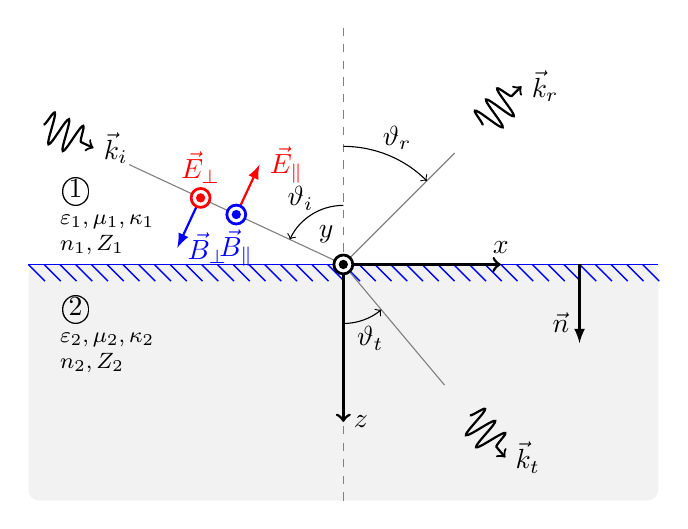
\begin{tikzpicture}[media/.style={font={\footnotesize}},wave/.style={decorate,decoration={snake,post length=1.4mm,amplitude=2mm,segment length=2mm},thick},
		interface/.style={
				% The border decoration is a path replacing decorator. 
				% For the interface style we want to draw the original path.
				% The postaction option is therefore used to ensure that the
				% border decoration is drawn *after* the original path.
				postaction={draw,decorate,decoration={border,angle=-45,
								amplitude=0.3cm,segment length=2mm}}},
	]
	% Round rectangle
	\fill[gray!10,rounded corners] (-4,-3) rectangle (4,0);
	% Interface
	\draw[blue,line width=.5pt,interface](-4,0)--(4,0);
	% Vertical dashed line
	\draw[dashed,gray](0,-3)--(0,3);
	% Coordinates system
	\draw(0,0.15)node[anchor=south east]{$y$};
	\draw[<->,line width=1pt] (2,0) node[above]{$x$}-|(0,-2) node[right]{$z$};
	% Incidence
	\draw[->,wave]
	(155:4.2cm)--(155:3.5cm)node[right]{$\vec{k}_i$};
	\draw[gray](0:0cm)--(155:3cm);
	\path (0,0)++(123:1cm)node{$\vartheta_i$};
	\draw[->](0,0.75)arc(90:155:.75cm);
	% EField
	\draw[red, -latex,thick](155:1.5)--+(65:0.7)node[right]{$\vec{E}_\parallel$};
	\filldraw[fill=white,draw=blue,line width=1pt](155:1.5)circle(.12cm) node[blue,below,yshift=-1.5]{$\vec{B}_\parallel$};
	\filldraw[fill=blue,draw=blue,line width=1pt](155:1.5)circle(.04cm);

	\draw[blue, -latex,thick](155:2)--+(245:0.7)node[right]{$\vec{B}_\perp$};
	\filldraw[fill=white,draw=red,line width=1pt](155:2)circle(.12cm) node[red,above,yshift=1.5]{$\vec{E}_\perp$};
	\filldraw[fill=red,draw=red,line width=1pt](155:2)circle(.04cm);

	% Transmission
	\draw[->,wave]
	(-50:2.5cm)--(-50:3.2cm)node[right]{$\vec{k}_t$};
	\draw[gray](0:0cm)--(-50:2cm);
	\path (0,0)++(-70:1cm)node{$\vartheta_t$};
	\draw[->] (0,-0.75) arc (-90:-50:.75cm);
	% Reflection
	\draw[->,wave]
	(45:2.5cm)--(45:3.2cm)node[right]{$\vec{k}_r$};
	\path (0,0)++(67:1.75cm) node{$\vartheta_r$};
	\draw[gray](0:0cm)--(45:2cm);
	\draw[->] (0,1.5)arc(90:45:1.5cm);
	% Media names
	\path[media] (-3,.6)  node[align=left]{{\normalsize\textcircled{1}\footnotesize}\\ $\varepsilon_1,\mu_1,\kappa_1$\\ $n_1, Z_1$}
	(-3,-.9) node[align=left]{{\normalsize\textcircled{2}\footnotesize}\\ $\varepsilon_2,\mu_2,\kappa_2$\\ $n_2, Z_2$};

	% $y$ axis
	\filldraw[fill=white,line width=1pt](0,0)circle(.12cm);
	\filldraw[fill=black,line width=1pt](0,0)circle(.04cm);
	% \draw[line width=.6pt] (0,0)
	%                       +(-135:.12cm) -- +(45:.12cm)
	%                       +(-45:.12cm) -- +(135:.12cm);

	\draw[thick,-latex] (3,0) -- (3,-1) node[anchor=south east]{$\vec{n}$};
\end{tikzpicture}}
  \end{minipage}
	   In diesem Abschnitt sollen \textbf{linear polarisierte ebene Wellen} am Übergang zweier Medien mit homogenen, linearen und isotropen Materialeigenschaften betrachtet werden. Der Wellenvektor der einfallenden Welle \(\vec{k}_i\) und Normalenvektor der Grenzfläche \(\vec{n}\) spannen die \textbf{Einfallsebene} auf. Ohne Beschränkung der Allgemeinheit kann \(\vec{n} = \vu{z}\) gesetzt werden (das Koordinatensystem kann beliebig rotiert werden).
	  Es werden folgende Indizes gewählt:
	  \begin{itemize}
	  	\item $i$ - inzident
	  	\item $r$ - reflektiert
	  	\item $t$ - transmittiert
	  \end{itemize} 
	  Weiterhin werden zwei Fälle unterschieden:
	  \begin{enumerate}
	  	\item \textbf{senkrechte Polarisation} ($\perp$,\enquote{horizontal}): $\vec{E}_i$ steht senkrecht zur Einfallsebene
	  	\item \textbf{parallele Polarisation} ($\parallel$,\enquote{vertikal}): $\vec{E}_i$ liegt in der Einfallsebene
	  \end{enumerate} 
	  Alle anderen Polarisationen können als Superposition der beiden Fälle angesehen werden ($\nearrow$\ref{poleb}). Außerdem soll harmonische Zeitabhängigkeit  angenommen werden (Fourier-Synthese möglich $\to$ keine echte Einschränkung), das heißt ausgeschrieben:
		        \begin{align}
			        \ubar{\vec{E}}_i(\vec{r} , t) & = \ubar{\vec{E}}_{0i}  \mathrm{e}^{\mathrm{j}(\omega_i t - \vec{k}_i \cdot \vec{r} )} & \vec{\ubar{B}}_i(\vec{r} , t) & = \frac{1}{\omega_i} \left(\vec{k}_i \times \ubar{\vec{E}}_i(\vec{r} , t)\right) \\
			        \ubar{\vec{E}}_r(\vec{r} , t) & = \ubar{\vec{E}}_{0r}  \mathrm{e}^{\mathrm{j}(\omega_r t - \vec{k}_r \cdot \vec{r} )} & \vec{\ubar{B}}_r(\vec{r} , t) & = \frac{1}{\omega_r} \left(\vec{k}_r \times \ubar{\vec{E}}_r(\vec{r} , t)\right) \\
			        \ubar{\vec{E}}_t(\vec{r} , t) & = \ubar{\vec{E}}_{0t}  \mathrm{e}^{\mathrm{j}(\omega_t t - \vec{k}_t \cdot \vec{r} )} & \vec{\ubar{B}}_t(\vec{r} , t) & = \frac{1}{\omega_t} \left(\vec{k}_t \times \ubar{\vec{E}}_t(\vec{r} , t)\right)
		        \end{align} 
Die Beziehungen für harmonische ebene Wellen sind in \ref{ebwellzsfg} zusammengefasst. Im folgenden wird $\kappa=0$ angenommen (also reelle Permittivität etc.). Wenn $\kappa\neq 0$ gelten sollte, müssen entsprechend der Betrachtungen in \ref{leitendeMed} einige Größen komplex geschrieben werden. Die Vorgehensweise und die resultierenden Gleichungen sind aber vollkommen analog. Das Verhalten von Feldern an Grenzflächen wurde in \ref{Grenz} untersucht und wird hier genutzt.
\subsection{Zusammenhänge der Kreisfrequenzen}
  Entsprechend den Ausführungen in \ref{Grenz} wird die Tangentialkomponente von \(\vec{E}\) betrachtet ($\nearrow$\ref{tanE}). Für \(z=0\) muss gelten:
		        \begin{equation}\label{tanEwellen}
			        \vec{n} \times \left( \ubar{\vec{E}}_{0t}  \mathrm{e}^{\mathrm{j}(\omega_t t - \vec{k}_t \cdot \vec{r} )} -\left( \ubar{\vec{E}}_{0i}  \mathrm{e}^{\mathrm{j}(\omega_i t - \vec{k}_i \cdot \vec{r} )} + \ubar{\vec{E}}_{0r}  \mathrm{e}^{\mathrm{j}(\omega_r t - \vec{k}_r \cdot \vec{r} )}\right)\right) \stackrel{!}{=} \vec{0}
		        \end{equation}
 Für \textbf{beliebige Zeitpunkte \(t \ne 0\) und \(\vec{r}  = \vec{0}\)} kann dies nur erfüllt werden, wenn gilt
		        \begin{equation}
			        \mathrm{e}^{\mathrm{j}\omega_i t} =  \mathrm{e}^{\mathrm{j}\omega_r t} = \mathrm{e}^{\mathrm{j}\omega_t t} \Rightarrow \boxed{\omega_i =\omega_r = \omega_t} \quad 
		        \end{equation}
		       Ein Sinus mit nicht verschwindender Amplitude kann unmöglich zu jedem Zeitpunkt gleich einem Sinus anderer Frequenz sein. Die \textbf{Kreisfrequenzen} \textbf{ändern} sich also \textbf{nicht}.
\subsection{Reflexions- und Brechungsgesetz}
		  Im gewählten Koordinatensystem (Einfallsebene ist $x-z-$Ebene) gilt durch Projektion:
		        \begin{equation}\begin{split}
				        \vec{k}_i &=  k_i \left( \sin\vartheta_i\vu{x} + \cos\vartheta_i\vu{z} \right)\\
				        \vec{k}_r &=  k_r \left( \cos\varphi_r\sin\vartheta_r\vu{x} + \sin\varphi_r\sin\vartheta_r\vu{y}  - \cos\vartheta_r\vu{z}\right) \\
				        \vec{k}_t &=  k_t \left( \cos\varphi_t\sin\vartheta_t\vu{x} + \sin\varphi_t\sin\vartheta_t\vu{y}  + \cos\vartheta_t\vu{z}\right)
			        \end{split}\end{equation}
		   Es wird ein Punkt an der Grenzfläche (\(z=0\)) betrachtet, dort gilt \(\vec{r}  = x\vu{x} + y\vu{y} \). Damit:
		        \begin{equation}\label{spwellort}\begin{split}
				        \vec{k}_i\cdot\vec{r}  &= x \underbrace{k_i \sin\vartheta_i }_{k_{ix}} + y\underbrace{0}_{k_{iy}} \\
				        \vec{k}_r \cdot\vec{r} &= x \underbrace{k_r\cos\varphi_r\sin\vartheta_r}_{k_{rx}} + y\underbrace{k_r\sin\varphi_r\sin\vartheta_r}_{k_{ry}}  \\
				        \vec{k}_t \cdot\vec{r} &=  x \underbrace{k_t  \cos\varphi_t\sin\vartheta_t}_{k_{tx}} + y\underbrace{k_t \sin\varphi_t\sin\vartheta_t}_{k_{ty}}
			        \end{split}\end{equation}
		  Setzt man in \ref{tanEwellen} \(t=0\), kann man die selbe Argumentation wie für die Frequenz für die $x$- und $y$-Komponente ($z=0$) durchziehen. Es muss also 
		  \begin{equation}
		  	\mathrm{e}^{-\mathrm{j}(k_{tx}x+k_{ty}y)}=		  	\mathrm{e}^{-\mathrm{j}(k_{ix}x+k_{iy}y)}=
		  			  	\mathrm{e}^{-\mathrm{j}(k_{rx}x+k_{ry}y)} \Rightarrow \boxed{k_{tx}=k_{ix}=k_{rx}  \text{ und } k_{ty}=k_{iy}=k_{ry}}
		  \end{equation}
		  gelten. Mit Koeffizientenvergleich in \ref{spwellort}:
		        \begin{equation}\begin{split}
			        x:&\quad k_i\sin\vartheta_i =  k_r\cos\varphi_r\sin\vartheta_r = k_t\cos\varphi_t\sin\vartheta_t \\
			       y:&\quad0= k_r\sin\varphi_r\sin\vartheta_r =  k_t\sin\varphi_t\sin\vartheta_t
		        \end{split}\end{equation}
		   Aus der \(y\)-Komponente folgt für \(\vartheta_r\ne 0\) und \(\vartheta_t\ne 0\): \begin{equation}
		   	\boxed{\varphi_r=\varphi_t=0}
		   \end{equation} 
		   Die \textbf{reflektierte} und \textbf{transmittierte} \textbf{Komponente} liegen also in der \textbf{Einfallsebene}.
		  Die Bedingung für die \(x\)-Komponente vereinfacht sich damit zu
		        \begin{equation}\label{vereinfx}
			        k_i\sin\vartheta_i =  k_r\sin\vartheta_r = k_t\sin\vartheta_t
		        \end{equation}
		  Die Beträge der Wellenvektoren sind durch die Materialien bestimmt:
		        \begin{equation}\begin{split}
				        k_i =  k_r &= \frac{2\pi}{\lambda_1} = \frac{\omega}{ v_{c_1}} = \omega\sqrt{\varepsilon_1\mu_1} = \frac{\omega}{c}\sqrt{\varepsilon_{r_1}\mu_{r_1}} = \frac{\omega}{c} n_1 = k_1\\
				        k_t &= \frac{2\pi}{\lambda_2} = \frac{\omega}{ v_{c_2}} = \omega\sqrt{\varepsilon_2\mu_2} = \frac{\omega}{c}\sqrt{\varepsilon_{r_2}\mu_{r_2}} = \frac{\omega}{c} n_2 = k_2
			        \end{split}\end{equation}
		  Einsetzen in \ref{vereinfx} ergibt zwei Gesetze:
\begin{align}
	\textbf{Reflexionsgesetz:} & & \Aboxed{\vartheta_i&=\vartheta_r}:=\vartheta_1\\
	\textbf{Brechungsgesetz nach Snellius:} & & \Aboxed{ n_1\sin\vartheta_1 &= n_2\sin\vartheta_2}\quad \text{ mit } \quad\vartheta_2:=\vartheta_t\label{snellius}
\end{align}
  \subsection{Reflexions- und Transmissionskoeffizienten}
  Es ist materialabhängig, wie stark eine elektromagnetische Welle reflektiert oder transmittiert wird. Bei solchen Betrachtungen muss man zwischen senkrechter und paralleler Polarisation unterscheiden. Das Vorgehen ist bei paralleler und senkrechter Polarisation analog. Die folgenden Grafiken verdeutlichen die Definitionsrichtungen der Größen und das gewählte Koordinatensystem. Es werden ebene Wellen betrachtet, das heißt $\vec{k}$, $\vec{E}$ und $\vec{B}$ bilden ein Rechtsdreibein. $\vec{k}$ sollte zudem sinnvollerweise in Ausbreitungsrichtung zeigen. Dennoch bleiben Freiheitsgrade, wie die anderen beiden Vektoren orientiert sind (bei senkrechter Polarisation bspw. $\vec{E}$ in die Ebene hinein oder aus der Ebene hinaus). Man kann gleichwertig mit anderen Definitionsrichtungen rechnen, die Ergebnisse würden sich physikalisch nicht unterscheiden. Was sich aber unterscheiden kann sind Rechengrößen wie der Reflektionsfaktor. Wenn man bspw. einen Phasensprung um $\pi$ durch Reflektion hat und den reflektierten Vektor antiparallel zum inzidenten definiert, dann ist der Reflektionskoeffizient positiv. Definiert man hingegen parallel, wäre der Reflektionskoeffizient positiv. Deshalb sollte man stets die Definitionen angeben, auf die man sich bezieht. \\
	  \begin{minipage}{.5\textwidth}
	\centering
	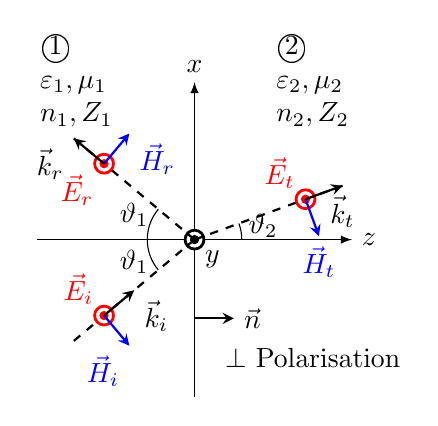
\begin{tikzpicture}
		\draw[-latex, thin] (-2,0) -- (2,0) node[anchor=west] {$z$};
		\draw[-latex, thin] (0,-2) -- (0,2) node[anchor=south] {$x$};
		\filldraw[fill=white,line width=1pt](0,0)circle(.12cm) node[anchor=north west]{$y$};
		\filldraw[fill=black,line width=1pt](0,0)circle(.04cm);
		\path (-1.5,2)  node[align=left]{{\normalsize\textcircled{1}}\\ $\varepsilon_1,\mu_1$\\ $n_1, Z_1$}
		(1.5,2) node[align=left]{{\normalsize\textcircled{2}}\\ $\varepsilon_2,\mu_2$\\ $n_2, Z_2$};
		\draw[dashed, thick] (0,0) -- +(20:2);
		\draw[dashed, thick] (220:2) -- (0,0);
		\draw[dashed, thick] (0,0) -- (140:2);
		\draw[thin] (0.6,0) arc (0:20:0.6) node[right,yshift=-1]{$\vartheta_2$};
		\draw[thin] (-0.6,0) arc (180:220:0.6) node[left,yshift=3]{$\vartheta_1$};
		\draw[thin] (-0.6,0) arc (180:140:0.6) node[left,yshift=-2]{$\vartheta_1$};

		\filldraw[fill=white,line width=1pt, draw=red](140:1.5)circle(.12cm) node[red, anchor=north east]{$\vec{E}_r$};
		\filldraw[fill=red,line width=1pt, draw=red](140:1.5)circle(.04cm);
		\draw[blue,-stealth, thick] (140:1.5) -- +(50:0.5) node[blue, anchor=north west]{$\vec{H}_r$};
		\draw[black,-stealth, thick] (140:1.5) -- +(140:0.5) node[anchor=north east]{$\vec{k}_r$};

		\filldraw[fill=white,line width=1pt, draw=red](220:1.5)circle(.12cm) node[red, anchor=south east]{$\vec{E}_i$};
		\filldraw[fill=red,line width=1pt, draw=red](220:1.5)circle(.04cm);
		\draw[blue,-stealth, thick] (220:1.5) -- +(310:0.5) node[blue, anchor=north east]{$\vec{H}_i$};
		\draw[black,-stealth, thick] (220:1.5) -- +(220:-0.5) node[anchor=north west]{$\vec{k}_i$};

		\filldraw[fill=white,line width=1pt, draw=red](20:1.5)circle(.12cm) node[red, anchor=south east]{$\vec{E}_t$};
		\filldraw[fill=red,line width=1pt, draw=red](20:1.5)circle(.04cm);
		\draw[blue,-stealth, thick] (20:1.5) -- +(-70:0.5) node[blue, anchor=north]{$\vec{H}_t$};
		\draw[black,-stealth, thick] (20:1.5) -- +(20:0.5) node[anchor=north]{$\vec{k}_t$};
		\draw (1.5,-1.5) node{$\perp$ Polarisation};
		\draw[-stealth,thick] (0,-1) -- (0.5,-1) node[anchor=west]{$\vec{n}$};
	\end{tikzpicture}
\end{minipage}
\begin{minipage}{.5\textwidth}
	\centering
	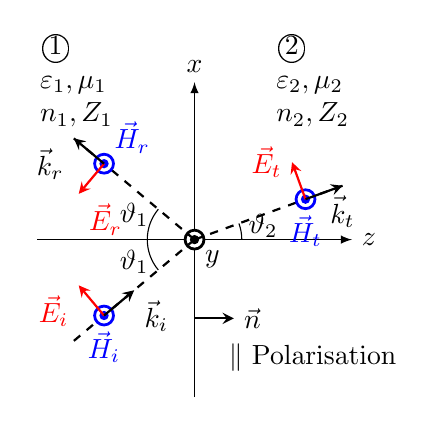
\begin{tikzpicture}
		\draw[-latex, thin] (-2,0) -- (2,0) node[anchor=west] {$z$};
		\draw[-latex, thin] (0,-2) -- (0,2) node[anchor=south] {$x$};
		\filldraw[fill=white,line width=1pt](0,0)circle(.12cm) node[anchor=north west]{$y$};
		\filldraw[fill=black,line width=1pt](0,0)circle(.04cm);
		\path (-1.5,2)  node[align=left]{{\normalsize\textcircled{1}}\\ $\varepsilon_1,\mu_1$\\ $n_1, Z_1$}
		(1.5,2) node[align=left]{{\normalsize\textcircled{2}}\\ $\varepsilon_2,\mu_2$\\ $n_2, Z_2$};
		\draw[dashed, thick] (0,0) -- +(20:2);
		\draw[dashed, thick] (220:2) -- (0,0);
		\draw[dashed, thick] (0,0) -- (140:2);
		\draw[thin] (0.6,0) arc (0:20:0.6) node[right,yshift=-1]{$\vartheta_2$};
		\draw[thin] (-0.6,0) arc (180:220:0.6) node[left,yshift=3]{$\vartheta_1$};
		\draw[thin] (-0.6,0) arc (180:140:0.6) node[left,yshift=-2]{$\vartheta_1$};

		\filldraw[fill=white,line width=1pt, draw=blue](140:1.5)circle(.12cm) node[blue, anchor=south west]{$\vec{H}_r$};
		\filldraw[fill=blue,line width=1pt, draw=blue](140:1.5)circle(.04cm);
		%\draw[line width=.6pt] (0,0) +(-135:.12cm) -- +(45:.12cm) +(-45:.12cm) -- +(135:.12cm); 
		\draw[red,-stealth, thick] (140:1.5) -- +(230:0.5) node[red, anchor=north west]{$\vec{E}_r$};
		\draw[black,-stealth, thick] (140:1.5) -- +(140:0.5) node[anchor=north east]{$\vec{k}_r$};

		\filldraw[fill=white,line width=1pt, draw=blue](220:1.5)circle(.12cm) node[blue, anchor=north,yshift=-2]{$\vec{H}_i$};
		\filldraw[fill=blue,line width=1pt, draw=blue](220:1.5)circle(.04cm);
		%\draw[blue, line width=.6pt] (220:1.5) +(-135:.12cm) -- +(45:.12cm) +(-45:.12cm) -- +(135:.12cm); 
		\draw[red,-stealth, thick] (220:1.5) -- +(130:0.5) node[anchor=north east]{$\vec{E}_i$};
		\draw[black,-stealth, thick] (220:1.5) -- +(220:-0.5) node[anchor=north west]{$\vec{k}_i$};

		\filldraw[fill=white,line width=1pt, draw=blue](20:1.5)circle(.12cm) node[blue, anchor=north,yshift=-2]{$\vec{H}_t$};
		\filldraw[fill=blue,line width=1pt, draw=blue](20:1.5)circle(.04cm);
		%\draw[line width=.6pt] (0,0) +(-135:.12cm) -- +(45:.12cm) +(-45:.12cm) -- +(135:.12cm); 
		\draw[red,-stealth, thick] (20:1.5) -- +(110:0.5) node[red, anchor=east]{$\vec{E}_t$};
		\draw[black,-stealth, thick] (20:1.5) -- +(20:0.5) node[anchor=north]{$\vec{k}_t$};
		\draw (1.5,-1.5) node{$\parallel$ Polarisation};
		\draw[-stealth,thick] (0,-1) -- (0.5,-1) node[anchor=west]{$\vec{n}$};
	\end{tikzpicture}
\end{minipage}
	  Im \textbf{Spezialfall}, dass $\vec{k}_i \parallel \vec{n}$, ist die Einfallsebene nicht eindeutig definiert. Man kann dann gleichwertig mit den Formeln für parallele und senkrechte Polarisation rechnen. Zu beachten ist dabei allerdings, wie die Vektoren definiert sind. So wird man feststellen, dass $\ubar{r}_\perp=-\ubar{r}_\parallel$ ist. Das liegt daran, dass der elektrische Feldvektor des reflektierten Felds im Fall der parallelen Polarisation antiparallel zu dem einfallenden elektrischen Feldvektor definiert ist und im Fall der senkrechten Polarisation parallel. Im parallel polarisierten Fall ist also $\vu{{E_i}}=-\vu{{E_r}}$, im senkrechten hingegen $\vu{{E_i}}=\vu{{E_r}}$, sodass mit $\ubar{r}_\perp=-\ubar{r}_\parallel$ die berechnete Feldstärke $\vec{\ubar{E}}_r$ in beiden Fällen gleich ist.
	  \subsubsection{Senkrechte Polarisation}
	Es wird das \(\vec{E}\)-Feld betrachtet, welches in $y$-Richtung orientiert ist. Die Wellenvektoren haben entsprechend der Grafik für  die folgenden Richtungen:
			        \begin{align}
				        \vu{{k_i}} & = \sin\vartheta_1\vu{x} + \cos\vartheta_1\vu{z} \nonumber \\
				        \vu{{k_r}} & = \sin\vartheta_1\vu{x} - \cos\vartheta_1\vu{z} \label{ekrgln} \\
				        \vu{{k_t}} & = \sin\vartheta_2\vu{x} + \cos\vartheta_2\vu{z} \nonumber
			        \end{align}
		Der Ortsvektor bei \(z=0
			        \) ist \(\vec{r}  = x\vu{x} + y \vu{y}\).
			   Aus der Stetigkeit der Tangentialkomponente von \(\vec{E}\) ($\nearrow$\ref{tanE}) folgt unter Beachtung von $\vu{z} \times \vu{y} = -\vu{x}$:
			        \begin{equation}\begin{split}
					        \vu{z} \times \left(\ubar{E}_{0i} \vu{y} \mathrm{e}^{-\mathrm{j} k_i x \sin\vartheta_1} + \ubar{E}_{0r} \vu{y} \mathrm{e}^{-\mathrm{j} k_r x \sin\vartheta_1}   \right) &= \vu{z} \times \ubar{E}_{0t} \vu{y} \mathrm{e}^{-\mathrm{j} k_t x \sin\vartheta_2}   \\
					        -\vu{x}  \left(\ubar{E}_{0i}  \mathrm{e}^{-\mathrm{j} k_i x \sin\vartheta_1} + \ubar{E}_{0r} \mathrm{e}^{-\mathrm{j} k_r x \sin\vartheta_1}   \right) &= -\vu{x}  \ubar{E}_{0t}  \mathrm{e}^{-\mathrm{j} k_t x \sin\vartheta_2}
				        \end{split}\end{equation}
			   Das gilt für beliebige Punkte auf der Grenzfläche. Für \(x=0\) folgt:
			        \begin{equation}\label{refltransbzh1}
				        \boxed{ \ubar{E}_{0i} + \ubar{E}_{0r}= \ubar{E}_{0t}}
			        \end{equation}
			       Gibt es zwei Grenzflächen, kann im gleichen Koordinatensstem offensichtlich nicht an beiden Grenzflächen $z=0$ gelten. Außerdem kommt es in diesem Fall zu Mehrfachreflexionen, also mathematisch zu einer Superpostion von unendlich vielen Phasoren. Diese Reihe kann man als einen einzigen resultierenden Phasor auffassen (die Superposition unendlich vieler gleichfrequenter Signale ergibt ein Signal dieser Frequenz mit bestimmter Amplitude und Phase). Anstatt die Reihen explizit hinzuschreiben, ist es möglich, direkt diese resultierenden Phasoren als Gesamtwelle an die Randbedingungen anzupassen.\\
			        Nun soll das $\vec{H}$-Feld betrachtet werden. Die Oberflächenstromdichte ist 0 ($\nearrow$Betrachtungen in \ref{skin}). Folglich ist nach \ref{tanH} ($J_A=0$):
			        \begin{equation}
			        	\vu{z}\times\left(\vec{H}_i+\vec{H}_r\right)=\vu{z}\times\vec{H}_t
			        \end{equation}
			        Nun kann man den Zusammenhang zwischen $H$ und $E$ über den Feldwellenwiderstand ansetzten ($\nearrow$\ref{ebwellzsfg}). Demnach ist:
			        \begin{equation}       	\vu{z}\times\left(\frac{1}{Z_1}\vu{{k_i}}\times\vec{E}_i+\frac{1}{Z_1}\vu{{k_r}}\times\vec{E}_r\right)=\vu{z}\times\frac{1}{Z_2}\vu{{k_t}}\times\vec{E}_t
			        \end{equation}
			   Die doppelten Kreuzprodukte kann man auflösen. Dafür wird \ref{grass}, \(\vu{z}\cdot \vec{E}_{irt}=0\) sowie \ref{ekrgln} genutzt:
			        \begin{align}
				        \frac{1}{Z_1}\left[   - \vec{E}_i\left(\vu{z}\cdot \vu{{k_i}}  \right)  - \vec{E}_r\left(\vu{z}\cdot \vu{{k_r}}  \right) \right] & = \frac{1}{Z_2}\left[   - \vec{E}_t\left(\vu{z}\cdot \vu{{k_t}}  \right)\right] \nonumber\\
				        \frac{1}{Z_1}\left[   - \cos\vartheta_1\vec{E}_i  +\cos\vartheta_1 \vec{E}_r \right]                                             & = -\frac{1}{Z_2} \cos\vartheta_2 \vec{E}_t                                    \nonumber  \\
				        \Aboxed{\frac{1}{Z_1}\left[   \cos\vartheta_1\ubar{E}_{0i}  -\cos\vartheta_1 \ubar{E}_{0r} \right]                               & = \frac{1}{Z_2} \cos\vartheta_2 \ubar{E}_{0t}}\label{refltransbzh2}
			        \end{align}
			   Mit \ref{refltransbzh1} und \ref{refltransbzh2} können der \textbf{Reflexions-} und der \textbf{Transmissionskoeffizient}
			        \begin{equation}
				        \underline{r}_\perp = \frac{\ubar{E}_{0r}}{\ubar{E}_{0i}} \qquad \underline{t}_\perp = \frac{\ubar{E}_{0t}}{\ubar{E}_{0i}} 
			        \end{equation}
			        bestimmt werden.
			   Aus \ref{refltransbzh1} ergibt sich:
			        \begin{equation}
				        \ubar{E}_{0i} + \ubar{E}_{0r}= \ubar{E}_{0t} \Rightarrow  1+ \frac{\ubar{E}_{0r}}{\ubar{E}_{0i}}= \frac{\ubar{E}_{0t}}{\ubar{E}_{0i}} \Rightarrow \boxed{1+\underline{r}_\perp = \underline{t}_\perp}
			        \end{equation}
			   Aus \ref{refltransbzh2} ergibt sich:
			        \begin{equation}
				        \frac{1}{Z_1}\left[   \cos\vartheta_1\ubar{E}_{0i}  -\cos\vartheta_1 \ubar{E}_{0r} \right] = \frac{1}{Z_2} \cos\vartheta_2 \ubar{E}_{0t} \Rightarrow  \boxed{Z_2\cos\vartheta_1\left(1-\underline{r}_\perp\right) = Z_1 \cos\vartheta_2\underline{t}_\perp}
			        \end{equation}
			   Hieraus ergeben sich durch umstellen Reflexions- und Transmissionskoeffizient (\textbf{Fresnelsche Beziehungen}) zu
			        \begin{align}
				        \Aboxed{\underline{r}_\perp                         & = \frac{Z_2\cos\vartheta_1-Z_1\cos\vartheta_2}{Z_1\cos\vartheta_2+Z_2\cos\vartheta_1}} \label{frenselsref}\\
				        1+\underline{r}_\perp = \Aboxed{\underline{t}_\perp & = \frac{2 Z_2\cos\vartheta_1}{Z_1\cos\vartheta_2+Z_2\cos\vartheta_1}}\label{frenselstrans}
			        \end{align}
			  Die Beziehungen gelten natürlich auch für komplexe Feldwellenwiderstände. Ein wichtiger Spezialfall ist der Übergang Luft-Metall. 
			   \begin{itemize}
			   	\item In \textbf{Luft} gilt ($\nearrow\ref{feldwellenwid}$): \(Z=Z_1\simeq 377 \mathrm{\Omega}\)
			   	\item Für \textbf{Metall} gilt: \({\displaystyle \ubar{Z}=\ubar{Z}_2 = \sqrt{\frac{\mu}{\underline{\varepsilon}}}  = \sqrt{\frac{\mu}{\varepsilon_0\left(\varepsilon_r -\mathrm{j}\frac{\kappa}{\varepsilon_0\omega}\right)}} \simeq (1+\mathrm{j})\sqrt{\frac{\mu\omega}{2\kappa}} \to \left|Z_2\right| \ll  377 \mathrm{\Omega}}\)\\
			   	$\quad\to$ Näherung für einen guten Leiter ($\kappa$ groß)
			   \end{itemize} 
			   Für typische Frequenzen gilt somit, dass alles reflektiert wird:
			        \begin{equation}
				         \underline{r}_\perp \simeq -1 \quad \underline{t}_\perp \simeq 0
			        \end{equation}

	  \subsubsection{Parallele Polarisation}
			   Die Herleitung von Reflexions- und Transmissionskoeffizienten für \textbf{parallele Polarisation} verläuft völlig analog und wird hier nicht wiederholt. Die Unterschiede in den \textbf{Fresnelschen Beziehungen} werden im direkten Vergleich deutlich ($\nearrow$\ref{frenselsref},\ref{frenselstrans}):
			        \begin{align}
				        \Aboxed{\underline{r}_\parallel   & = \frac{Z_1\cos\vartheta_1-Z_2\cos\vartheta_2}{Z_2\cos\vartheta_2+Z_1\cos\vartheta_1}} \\
				        \frac{Z_2}{Z_1}\left(1+\underline{r}_\parallel\right)=\frac{\cos\vartheta_1}{\cos\vartheta_2}\left(1-\underline{r}_\parallel\right)
				        = \Aboxed{\underline{t}_\parallel & = \frac{2 Z_2\cos\vartheta_1}{Z_2\cos\vartheta_2+Z_1\cos\vartheta_1}}
			        \end{align}
		 Für den Übergang Luft-Metall folgt hier (es ist im Gegensatz zu der senkrechten Polarisation kein Phasensprung nötig, was deutlich wird wenn man sich \ref{tanE} vergegenwärtigt):
			        \begin{equation}
				        \underline{r}_\parallel \simeq +1 \quad \underline{t}_\parallel \simeq 0
			        \end{equation}
	  \subsubsection{Senkrechte und parallele Polarisation, Schreibweise mit $n$}
		  Mit \(Z=\sqrt{\frac{\mu}{\varepsilon}}\) und \(n=\sqrt{\varepsilon_r\mu_r}\) folgt \(Z = \frac{\mu c}{n}\), so dass für die Reflexions- und Transmissionskoeffizienten folgt
			        \begin{align}
				        \Aboxed{\underline{r}_\perp     & = \frac{n_1\cos\vartheta_1-\frac{\mu_1}{\mu_2} n_2\cos\vartheta_2}{n_1\cos\vartheta_1+\frac{\mu_1}{\mu_2} n_2\cos\vartheta_2}}  & \Aboxed{\underline{t}_\perp     & = \frac{2 n_1\cos\vartheta_1}{n_1\cos\vartheta_1+\frac{\mu_1}{\mu_2} n_2\cos\vartheta_2}} \\
				        \Aboxed{\underline{r}_\parallel & = \frac{-n_1\cos\vartheta_2+\frac{\mu_1}{\mu_2} n_2\cos\vartheta_1}{n_1\cos\vartheta_2+\frac{\mu_1}{\mu_2} n_2\cos\vartheta_1}} & \Aboxed{\underline{t}_\parallel & = \frac{2 n_1\cos\vartheta_1}{n_1\cos\vartheta_2+\frac{\mu_1}{\mu_2} n_2\cos\vartheta_1}}
			        \end{align}
			  Wichtiger Spezialfall: \textbf{\(\mu_1 = \mu_2\)}, z.B. beide unmagnetisch
			        \begin{align}
				        \Aboxed{\underline{r}_\perp     & = \frac{n_1\cos\vartheta_1- n_2\cos\vartheta_2}{n_1\cos\vartheta_1+ n_2\cos\vartheta_2}} & \Aboxed{\underline{t}_\perp     & = \frac{2 n_1\cos\vartheta_1}{n_1\cos\vartheta_1+ n_2\cos\vartheta_2}} \\
				        \Aboxed{\underline{r}_\parallel & = \frac{-n_1\cos\vartheta_2+n_2\cos\vartheta_1}{n_1\cos\vartheta_2+ n_2\cos\vartheta_1}} & \Aboxed{\underline{t}_\parallel & = \frac{2 n_1\cos\vartheta_1}{n_1\cos\vartheta_2+ n_2\cos\vartheta_1}}
			        \end{align}
	  \subsubsection{Senkrechte und parallele Polarisation, Schreibweise mit \(\vartheta_1,\;\vartheta_2\)}
			  Im Falle \(\mu_1 = \mu_2\) können die Fresnelschen-Beziehungen mit Hilfe des Brechungsgesetzes \(n_1\sin\vartheta_1=n_2\sin\vartheta_2\) auch nur mit den Winkeln geschrieben werden:
			        \begin{equation}\label{frenselvereinf}\begin{split}
					        \Aboxed{\underline{r}_\perp &= \frac{\cos\vartheta_1- \frac{\sin\vartheta_1}{\sin\vartheta_2}\cos\vartheta_2}{\cos\vartheta_1+ \frac{\sin\vartheta_1}{\sin\vartheta_2}\cos\vartheta_2} = \frac{\sin\left(\vartheta_2-\vartheta_1\right)}{\sin\left(\vartheta_1+\vartheta_2\right)}}\\
					        \Aboxed{\underline{t}_\perp &= \frac{2 \cos\vartheta_1}{\cos\vartheta_1+ \frac{\sin\vartheta_1}{\sin\vartheta_2}\cos\vartheta_2} = \frac{2\sin\vartheta_2\cos\vartheta_1}{\sin\left(\vartheta_1+\vartheta_2\right)}} \\
					        \Aboxed{\underline{r}_\parallel &= \frac{-\cos\vartheta_2+ \frac{\sin\vartheta_1}{\sin\vartheta_2}\cos\vartheta_1}{\cos\vartheta_2+ \frac{\sin\vartheta_1}{\sin\vartheta_2}\cos\vartheta_1}=\frac{\tan\left(\vartheta_1-\vartheta_2\right)}{\tan\left(\vartheta_1+\vartheta_2\right)}}\\
					        \Aboxed{\underline{t}_\parallel &= \frac{2 \cos\vartheta_1}{\cos\vartheta_2+ \frac{\sin\vartheta_1}{\sin\vartheta_2}\cos\vartheta_1}= \frac{2\sin\vartheta_2\cos\vartheta_1}{\sin\left(\vartheta_1+\vartheta_2\right) \cos\left(\vartheta_1-\vartheta_2\right)}}
				        \end{split}\end{equation}
  \subsection{Verschwinden der Reflexion -- Brewster-Winkel}
		  Aus \ref{frenselvereinf} können die Bedingungen für das \textbf{Verschwinden der Reflexion} abgelesen werden (beachte die vereinfachende Annahme \(\mu_1 = \mu_2\)). Es gilt demnach:
		        \begin{align}
			        \underline{r}_\perp & = \frac{\sin\left(\vartheta_2-\vartheta_1\right)}{\sin\left(\vartheta_1+\vartheta_2\right)} & \underline{r}_\parallel & = \frac{\tan\left(\vartheta_1-\vartheta_2\right)}{\tan\left(\vartheta_1+\vartheta_2\right)}
		        \end{align}
		        Es gibt folgende Möglichkeiten, damit keine Reflexion auftritt ($r=0$):
		   \begin{enumerate}
		   	\item Bei $\parallel$ und $\perp$: $\ubar{r}=0$ bei $\vartheta_1=\vartheta_2\Leftrightarrow n_1=n_2\Leftrightarrow$ \textbf{optisch gleiches Material}
		   	\item \textbf{Nur} $\parallel$: $\ubar{r}_\parallel=0$ bei $\vartheta_1+\vartheta_2=\frac{\pi}{2}\Rightarrow \vec{\bm{k_r}} \perp \vec{\bm{k_t}}$
		   	\begin{itemize}
		   		\item[] Nach dem Brechungsgesetz von Snellius ($\nearrow$\ref{snellius}) gilt in diesem Fall:		   	
		   	\begin{equation}
		   		\frac{\sin\vartheta_1}{\sin\vartheta_2} = \frac{\sin\vartheta_1}{\sin\left(\frac{\pi}{2}-\vartheta_1\right)} = \frac{\sin\vartheta_1}{\cos\vartheta_1} = \boxed{\tan\vartheta_1=\frac{n_2}{n_1} }
		   	\end{equation}
		   	\item[]$\vartheta_{1}$ nennt man \textbf{Brewsterscher Polarisationswinkel}.
		   	\item[]Die Reflexion einer beliebig polarisierten Welle, die unter diesem Winkel auf die Grenzfläche trifft, ist somit senkrecht polarisiert (es wird nichts paralleles reflektiert). So kann man einen \textbf{Polarisator} realisieren oder Brechzahlen bestimmen.
		   	\end{itemize}
		   \end{enumerate}
  \subsection{Totalreflexion}
		  Nach dem Brechungsgesetz von Snellius ($\nearrow$\ref{snellius}) gilt beim Übergang zum \textbf{optisch dichteren Medium}: \(n_1 < n_2\Rightarrow \vartheta_1 > \vartheta_2\). Beim Übergang zum \textbf{optisch dünnerem Medium} gilt hingegen \(n_1 > n_2\Rightarrow \vartheta_1 < \vartheta_2\). In diesem Fall wird bei Vergrößerung von \(\vartheta_1\) irgendwann \(\vartheta_2 = \frac{\pi}{2}\) erreicht. Es wird dann nichts mehr transmittiert, man spricht von \textbf{Totalreflexion}. Der \textbf{Grenzwinkel der Totalreflexion} \(\vartheta_{1G}\) ist bestimmt durch ($\vartheta_2 = \frac{\pi}{2}$):
			              \begin{equation}
				              \boxed{\sin\vartheta_{1G} = \frac{n_2}{n_1}}
			              \end{equation}
			              \begin{center}
				              \begin{tikzpicture}
	\clip  (-5,-1.5) rectangle (5,1.5);
	\path [name path=unten] (-5,-1.5) -- (5,-1.5);
	\path [name path=mitte] (-5,0) -- (5,0);
	\path [name path=oben] (-5,1.5) -- (5,1.5);
	\path [name path=right] (5,-2) -- (5,2);
	\draw[thick] (-5,0) -- (5,0);
	\draw[fill=gray, opacity=0.3] (-5,-1.5) rectangle (5,0);
	\draw[fill=blue, opacity=0.2] (-5,0) rectangle (5,1.5);
	\path (-4.3,.6)  node[align=left]{{\normalsize\textcircled{2}}\\ $n_2=1.0$}
	(-4.3,-.9) node[align=left]{{\normalsize\textcircled{1}}\\ $n_1=1.3$};
	\draw[thin,dashed] (-2.8,-1.5) -- (-2.8,1.5);
	\draw[thin,dashed] (0,-1.5) -- (0,1.5);
	\draw[thin,dashed] (3.5,-1.5) -- (3.5,1.5);

	% 20
	\path [name path=ineins] (-2.8,0) -- +(250:4);  % 20
	\path [name path=refeins] (-2.8,0) -- +(290:4); % 20
	\path [name path=traeins] (-2.8,0) -- +(54.7:4); % 35.3
	\draw[name intersections={of=unten and ineins, by=u1}] [red, thick, -latex] (u1) -- (-2.8,0);
	\draw[name intersections={of=unten and refeins, by=u2}] [red, thick, -latex] (-2.8,0) --(u2);
	\draw[name intersections={of=oben and traeins, by=o1}] [red, thick, -latex] (-2.8,0) --(o1);
	\draw[thin, -stealth] (-2.8,-1) arc (270:250:1) node[below,xshift=2,yshift=-2]{$20^o$};
	\draw[thin, -stealth] (-2.8,-1) arc (270:290:1) node[below,xshift=-2,yshift=-2]{$20^o$};
	\draw[thin, -stealth] (-2.8,1) arc (90:54.7:1) node[above,xshift=-2,yshift=5]{$35.3^o$};
	% Grenzwinkel = 50.3
	\path [name path=inzwei] (0,0) -- +(219.7:4);  % 50.3
	\path [name path=refzwei] (0,0) -- +(-39.7:4); % 50.3
	%\path [name path=trazwei] (0,0) -- +(0:4); % 90
	\draw[name intersections={of=unten and inzwei, by=u3}] [red, thick, -latex] (u3) -- (0,0);
	\draw[name intersections={of=unten and refzwei, by=u4}] [red, thick, -latex] (0,0) -- (u4);
	\draw[red, thick, -latex] (0,0) -- +(0:1.5);
	\draw[thin, -stealth] (0,-1) arc (270:219.7:1) node[below,xshift=5,yshift=-8]{$50.3^o$};
	\draw[thin, -stealth] (0,-1) arc (270:320.3:1) node[below,xshift=-5,yshift=-8]{$50.3^o$};
	\draw[thin, -stealth] (0,1) arc (90:0:1) node[above,xshift=-14,yshift=7]{$90^o$};
	% 60
	\path [name path=indrei] (3.5,0) -- +(210:4);  % 60
	\path [name path=refdrei] (3.5,0) -- +(330:4); % 60
	\draw[name intersections={of=unten and indrei, by=u5}] [red, thick, -latex] (u5) -- (3.5,0);
	\draw[name intersections={of=refdrei and right, by=u6}] [red, thick, -latex] (3.5,0) -- (u6);
	\draw[thin, -stealth] (3.5,-1) arc (270:210:1) node[below,xshift=5,yshift=-10]{$60^o$};
	\draw[thin, -stealth] (3.5,-1) arc (270:330:1) node[below,xshift=-5,yshift=-10]{$60^o$};
\end{tikzpicture}
			              \end{center}
		Anwendungen sind Lichtwellenleiter (Glasfaser), wo durch die vollständige Reflexion wenig Energie verloren geht, und Reflexionsprismen. Für den \textbf{Grenzwinkel der Totalreflexion}  gilt beim \textbf{Übergang in ein optisch dünneres Medium}:
			        \begin{equation}
				        \sin\vartheta_{1G} = \frac{n_2}{n_1} \Rightarrow \frac{n_1}{n_2}\sin\vartheta_{1G} = 1 \Rightarrow \boxed{\frac{n_1}{n_2}\sin\vartheta_{1} > 1 \text{ für } \vartheta_{1}>\vartheta_{1G}}
			        \end{equation}
			  Es wird \(\vec{k}_t\) betrachtet ($\nearrow$\ref{ekrgln}):
			        \begin{equation}\begin{split}
					        \vec{k}_t= k_2 \vu{{k_t}} &=  k_2 \left( \sin\vartheta_2\vu{x} +   \cos\vartheta_2\vu{z}\right) \\
					        &=  k_2 \left(\frac{n_1}{n_2} \sin\vartheta_1\vu{x} \pm \sqrt{\left(1-   \sin^2\vartheta_2\right)}\;\vu{z}\right)\\
					        &=  k_2 \left(\frac{n_1}{n_2} \sin\vartheta_1\vu{x} \pm \sqrt{\left(1-  \underbrace{\left(\frac{n_1}{n_2}\right)^2 \sin^2\vartheta_1}_{>1}\right)}\;\vu{z}\right)\\
					        &=  k_2 \left(\frac{n_1}{n_2} \sin\vartheta_1\vu{x} \pm \mathrm{j}\sqrt{\left( \left(\frac{n_1}{n_2}\right)^2 \sin^2\vartheta_1-1\right)}\;\vu{z}\right)\\
					        &= \beta \vu{x} \pm \mathrm{j}\alpha \vu{z}
				        \end{split}\end{equation}
	 Für das elektrische Feld im Medium 2 ergibt sich mit diesem Wellenvektor und dem Transmissionskoeffizienten \(t\):
			        \begin{align}
				        \ubar{\vec{E}}_t & = t \ubar{E}_{0i}  \mathrm{e}^{\mathrm{j}\left(\omega t - \vec{k}_t\cdot\vec{r}  \right)} \vu{{E_t}}                                                             \nonumber\\
				                         & = t \ubar{E}_{0i}  \mathrm{e}^{\pm\alpha z}  \mathrm{e}^{\mathrm{j}\left(\omega t - \beta x \right)}\vu{{E_t}} \quad\quad |\text{\(+\alpha z\) physikalisch unmöglich}  \\
				                         & = t \ubar{E}_{0i}  \mathrm{e}^{-\alpha z}  \mathrm{e}^{\mathrm{j}\left(\omega t - \beta x \right)}\vu{{E_t}}\nonumber 
			        \end{align}
			        Es gibt also einen exponentiellen Abfall in $z$-Richtung (hinein in das Medium) bei einer Wellenausbreitung in $x$-Richtung (entlang der Oberfläche). Für den Poynting-Vektor ergibt sich unter Nutzung von $\vec{\ubar{k}}_t = \beta \vu{x} - \mathrm{j}\alpha \vu{z}$:
			        \begin{align}
				        \vec{\ubar{S}} & = \frac{1}{2} \ubar{\vec{E}}_t \times \vec{\ubar{H}}_t^\star = \frac{1}{2 Z_2} \ubar{\vec{E}}_t \times \left(\vu{{k_t}}^\star \times \ubar{\vec{E}}_t^\star\right) = \frac{1}{2 Z_2} \left|\ubar{\vec{E}}_t\right|^2 \vu{{k_t}}^\star \\
				        & = \frac{1}{2 Z_2 k_2} \left|t \ubar{E}_{0i} \right|^2  \mathrm{e}^{-2\alpha z}\left( \beta \vu{x} +\mathrm{j}\alpha \vu{z}\right)
			        \end{align}
			  Es gibt also einen Wirkleistungsfluss in $x$-Richtung (entlang der Oberfläche) und Blindleistungsfluss in $z$-Richtung (in das Medium hinein). Das Medium 2 ist also nicht feldfrei. Es gibt eine Welle, die entlang der Oberfläche läuft und in $z$-Richtung eindringt, aber dort exponentiell gedämpft wird.		   Wird im Bereich des exponentiell abfallenden Feldes wieder ein Ausbreitungsmedium gebracht, so ergibt sich wieder eine transmittierte Welle (die Totalreflektion wird verhindert und ist dann ganz frustriert:(). Man spricht von \textbf{frustrierter Totalreflexion}. In diesem Fall sehen die elektromagnetischen Felder anders aus, es gibt einen Wirkleistungsfluss auch in $z$-Richtung. Es gibt formal eine große Übereinstimmung mit dem quantenmechanischen Tunneleffekt.
 \section{Inhomogene Wellengleichung - Erzeugung von Wellen}\label{erzemwell}
 \subsection{Greensche Funktion und retardierte Potentiale}
		  Im Abschnitt \ref{emwellgrdl} wurde bereits die Entkopplung der Maxwell-Gleichungen in ihrer allgemeinen Form betrachtet. Der Weg über die Felder ist für die folgenden Betrachtungen sehr kompliziert, deshalb ist es üblich über die Potentiale zu gehen. Definiert man \textbf{Vektorpotential} wie in \ref{potadef} und \textbf{Skalarpotential} wie in \ref{potsdef}, dann ergeben sich in \textbf{Coulomb-Eichung} die Bestimmungsgleichungen \ref{bestvekcoul} sowie \ref{bestskalcoul} und in \textbf{Lorenz-Eichung} \ref{bestvekpotlor} sowie \ref{bestskalarpotlor}. Dabei handelt es sich um inhomogene partielle Differentialgleichungen, die mit dem Formalismus der Greenschen Funktionen gelöst werden können ($\nearrow$\ref{greenfkt}).
		  Für den Wellenoperator kann die \textbf{Greensche-Funktion} folgendermaßen angegeben werden:
		  \begin{equation}\label{greenWell}
		  	\boxed{ G(\vec{r} -\vec{r}^\prime , t - t')=G_\mathrm{ret}(\vec{r} -\vec{r}^\prime , t - t') = \frac{1}{4\pi |\vec{r} -\vec{r}^\prime |}\delta\left(\frac{|\vec{r} -\vec{r}^\prime |}{ v_\mathrm{c}}-(t-t')\right) = \frac{\delta(t'-t_\mathrm{ret})}{4\pi |\vec{r} -\vec{r}^\prime |}}
		  \end{equation}
		  Hierbei ist 
		  \begin{equation}
		  	\boxed{t_\mathrm{ret} = t - \frac{|\vec{r} -\vec{r}^\prime |}{ v_\mathrm{c}}}
		  \end{equation} 
		  die \textbf{retardierte Zeit} und \(G_\mathrm{ret}\) die \textbf{retardierte Greensche Funktion}. Es gibt formal auch \textbf{avancierte} Lösungen ($t_\mathrm{av} = t - \frac{|\vec{r} +\vec{r}^\prime |}{ v_\mathrm{c}}$), diese sind aber nicht kausal, die Wirkung würde vor der Ursache in Erscheinung treten. Eine wichtige Erkenntnis daraus ist, dass es auch Lösungen der Maxwell-Gleichungen gibt, welche physikalisch nicht beobachtbare Phänomene beschreiben. Die \href{https://en.wikipedia.org/wiki/Jefimenko%27s_equations}{Gleichungen von Jefimenko} hingegen ergeben nur kausale Lösungen.\\
		   Die Lösung der inhomogenen Wellengleichung in Lorenz-Eichung sind damit dann die \textbf{retardierten Potentiale} ($\nearrow$ \ref{skalarpotlor},\ref{vekpotlor}):
		  \begin{align}
		  	\Aboxed{\phi_{{L}}(\vec{{r}}, {t})&=\frac{1}{4 \pi \varepsilon_{0}} \iiint \frac{\rho_\text{V}\left(\vec{{r}}^{\prime}, {t}_{\text{ret}}\right)}{\left|\vec{{r}}-\vec{{r}}^{\prime}\right|} \dd^3 {r}^{\prime}}\\
		  	\Aboxed{\vec{{A}}_{{L}}(\vec{{r}}, {t})&=\frac{\mu_{0}}{4 \pi} \iiint \frac{\vec{{J}}\left(\vec{{r}}^{\prime}, {t}_{\text{ret}}\right)}{\left|\vec{{r}}-\vec{{r}}^{\prime}\right|} \dd^3 {r}^{\prime}}
		  \end{align}
		   Bei retardierten Potentialen ist die Lösung wegen Retardierung in der Regel schwierig (für die Felder insbesondere die Integrale schwierig). Vereinfachen lässt sich das ganze in der Nahzone, wo die Retardierung vernachlässigt werden kann, und in der Fernzone, wo die Laufzeit von jedem Quellpunkt zum Beobachtungspunkt näherungsweise gleich ist ($\nearrow$\ref{strahlungszonen}).
		        \begin{center}
			        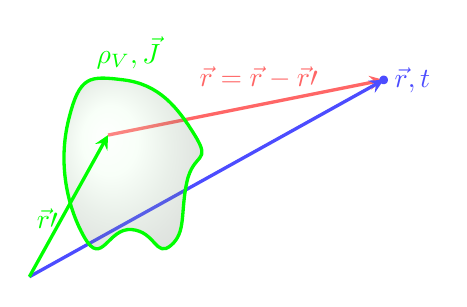
\begin{tikzpicture}[line width = 1.2pt, line join=round,>=stealth]
	% Differenzvektor R
	\draw [->, color=red!60] (1,1.8) -- (4.5,2.5);
	\draw [color=red!60] (3.8,2.25) node[anchor=south east] {$\vec{r}  = \vec{r}  - \vec{r}\prime  $};
	% Aufpunkt
	\draw [->,color=blue!70] (0,0) -- (4.5,2.5) node[anchor=west] {$\vec{r} , t$};
	\filldraw [color=blue!70] (4.5,2.5) circle (1pt);
	% Ladungsdichte
	\coordinate (a) at (2.1,1.8);
	\coordinate (b) at (2,1.2);
	\coordinate (c) at (1.8,0.4);
	\coordinate (d) at (1.3,0.6);
	\coordinate (e) at (0.7,0.5);
	\coordinate (f) at (0.5,2);
	\coordinate (g) at (1.2,2.5);
	\shade[ball color=white!10!green!20,opacity=0.20] plot [smooth cycle, tension = 1] coordinates {(a) (b) (c) (d) (e) (f) (g)};
	\draw [color=green] plot [smooth cycle, tension = 1] coordinates {(a) (b) (c) (d) (e) (f) (g)} node [sloped, above] {\ $ \rho_\text{V}, \vec{J} $};
	\draw [->,color=green] (0,0) -- (1,1.8);
	\draw [color=green] (0.5,1.0) node[anchor=north east] {$ \vec{r}\prime  $};
\end{tikzpicture}
		        \end{center}
		   Die Zeit \(\frac{|\vec{r} -\vec{r}^\prime |}{ v_\mathrm{c}}\) ist gerade die \textbf{Laufzeit} vom Quellpunkt $\vec{r}^\prime$ zum Beobachtungspunkt $\vec{r}$. Wenn also ein Feld (die Wirkung) am Ort $\vec{r}$ und zu einer Zeit $t$ beobachtet wird, dann muss man die Ursache am Ort $\vec{r}^\prime$ zu der Zeit $t_\mathrm{ret} = t - \frac{|\vec{r} -\vec{r}^\prime |}{ v_\mathrm{c}}$ beobachten, weil die Information eine gewisse Zeit benötigt, um sich auszubreiten. Eine quasistationäre Betrachtung wird dann möglich, wenn die Retardierung vernachlässigt werden kann ($\nearrow$\ref{quasistat}).
  \subsection{Strahlungszonen}\label{strahlungszonen}
	   Die Quellen \(\rho_\text{V}, \vec{J}\) seien nur innerhalb einer \textbf{Kugel mit Durchmesser \(d\)} von Null verschieden. Die Beschränkung auf ein räumlich begrenztes Gebiet ist naheliegend, häufig werden Wellen an Antennen erzeugt und propagieren dann. Es genügt die Betrachtung des Vektorpotentials, mit \ref{potadef} und \ref{durchf} mit $\vec{J}=0$ können dann außerhalb der Kugel alle Felder ausgerechnet werden. Zudem wir \textbf{harmonische Zeitabhängigkeit} betrachtet:
		        \begin{equation}\begin{split}
				        \vec{J} (\vec{r}^\prime , t) &= \re{\ubar{\vec{J}}(\vec{r}^\prime ) \mathrm{e}^{\mathrm{j}\omega t}} \\
				        \vec{J} (\vec{r}^\prime , t-\frac{|\vec{r} -\vec{r}^\prime |}{ v_\mathrm{c}}) &= \re{\ubar{\vec{J}}(\vec{r}^\prime ) \mathrm{e}^{\mathrm{j}\omega t} \mathrm{e}^{-\mathrm{j}\omega \frac{|\vec{r} -\vec{r}^\prime |}{ v_\mathrm{c}}}} \stackrel{v_\mathrm{c}=v_\mathrm{p}}{=} \re{\ubar{\vec{J}}(\vec{r}^\prime ) \mathrm{e}^{\mathrm{j}\omega t} \mathrm{e}^{-\mathrm{j} k |\vec{r} -\vec{r}^\prime |}}
			        \end{split}\end{equation}
		  Damit gilt für das komplexe Vektorpotential (hier wurde wieder auf $\mathrm{e}^{\mathrm{j}\omega t}$ normiert):
		        \begin{equation}\label{kompvekpot}
			        \boxed{%
			        \vec{\ubar{A}} (\vec{r} ) = \frac{\mu}{4\pi} \iiint\limits_V \frac{ \mathrm{e}^{-\mathrm{j} k |\vec{r} -\vec{r}^\prime |}}{|\vec{r} -\vec{r}^\prime |} \ubar{\vec{J}}(\vec{r}^\prime ) \dd^3  r^\prime}
		        \end{equation}
		   Hierbei ist
		        \(\tilde{G}_\mathrm{ret}(\vec{r} -\vec{r}^\prime ,  k) = \frac{1}{4\pi} \frac{ \mathrm{e}^{-\mathrm{j} k |\vec{r} -\vec{r}^\prime |}}{|\vec{r} -\vec{r}^\prime |}\)
		        die retardierte Greensche-Funktion im Bildraum mit \( k = \frac{\omega}{ v_\mathrm{c}} = \omega\sqrt{\varepsilon\mu}\). Nun sollen noch nähernde Vereinfachungen für dieses Integral betrachtet werden.
	  \begin{center}
		  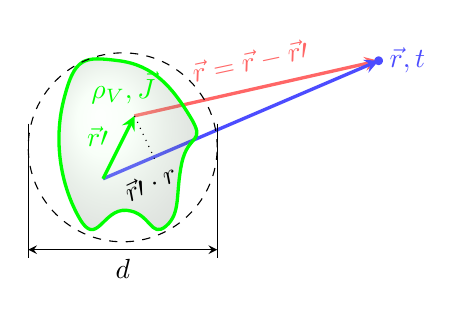
\begin{tikzpicture}[line width = 1.2pt, line join=round,>=stealth]
	% Differenzvektor R
	\draw [->, color=red!60] (1.4,1.8) -- (4.5,2.5);
	\draw [color=red!60] (3.8,2.4) node[anchor=south east, rotate=12] {$\vec{r}  = \vec{r}  - \vec{r}\prime  $};
	% Aufpunkt
	\draw [->,color=blue!70] (1,1) -- (4.5,2.5) node[anchor=west] {$\vec{r} , t$};
	\filldraw [color=blue!70] (4.5,2.5) circle (1pt);
	% Ladungsdichte
	\coordinate (a) at (2.1,1.8);
	\coordinate (b) at (2,1.2);
	\coordinate (c) at (1.8,0.4);
	\coordinate (d) at (1.3,0.6);
	\coordinate (e) at (0.7,0.5);
	\coordinate (f) at (0.5,2);
	\coordinate (g) at (1.2,2.5);
	\shade[ball color=white!10!green!20,opacity=0.20] plot [smooth cycle, tension = 1] coordinates {(a) (b) (c) (d) (e) (f) (g)};
	\draw [color=green] plot [smooth cycle, tension = 1] coordinates {(a) (b) (c) (d) (e) (f) (g)} node [sloped, below] {\ $ \rho_\text{V}, \vec{J} $};
	\draw [->,color=green] (1,1) -- (1.4,1.8);
	\draw [color=green] (1.2,1.8) node[anchor=north east] {$ \vec{r}\prime  $};
	\draw [dotted, thin] (1.4,1.8) -- +(-65:0.6) node[below,rotate=25,xshift=-5]{$\vec{r}\prime \cdot\vu{r}$};
	\draw[dashed,thin] (1.25,1.4) circle (1.2cm);
	\draw[thin] (0.05,1.7) -- (0.05,0);
	\draw[thin] (2.45,1.7) -- (2.45,0);
	\draw[thin, <->] (0.05, 0.1) -- (2.45, 0.1) node[midway, below]{$d$};
\end{tikzpicture}
	  \end{center}
		  Als Näherung für \(|\vec{r} | \gg d > |\vec{r}^\prime |\) gilt:
		        \begin{equation}\begin{split}
				        |\vec{r}  - \vec{r}^\prime | &\simeq |\vec{r} | - \vec{r}^\prime \cdot\vu{r} = r \left(1 - \frac{\vu{r}\cdot \vec{r}^\prime }{r} \right)\\
				       \left.\frac{1}{1-x}\right|_{x \ll 1}\simeq 1+x \Rightarrow \frac{1}{|\vec{r}  - \vec{r}^\prime |} &\simeq \frac{1}{r} \left( 1 +\frac{\vu{r}\cdot \vec{r}^\prime }{r} \right)
			        \end{split}\end{equation}
	Damit können 3 \textbf{Strahlungszonen} unterschieden werden:
	  \begin{enumerate}
		  \item In der \textbf{Nahzone} (statische Zone) gilt \(d \ll r \ll \lambda\). Es gibt \textbf{keine Retardierung}, weil:
		        \begin{equation}
			        \mathrm{e}^{-\mathrm{j} k |\vec{r} -\vec{r}^\prime |} \simeq  \mathrm{e}^{-\mathrm{j}\frac{2\pi}{\lambda}r \left(1 - \frac{\vu{r}\cdot \vec{r}^\prime }{r} \right) } \simeq  \mathrm{e}^{-\mathrm{j}0} =1  
		        \end{equation}
		  \item In der \textbf{Fernzone} (Strahlungszone) gilt \(d \ll r\) und \(\lambda \ll r\). Es gibt die \textbf{gleiche Retardierung} für alle $\vec{r}^\prime$, weshalb die Retardierung vor das Integral gezogen werden kann: 
		        \begin{equation}
			        \mathrm{e}^{-\mathrm{j} k |\vec{r} -\vec{r}^\prime |} \simeq  \mathrm{e}^{-\mathrm{j} k r} 
		        \end{equation}
		\item Dazwischen liegen die \textbf{Übergangszonen}. Es gilt \(d \simeq r\) und/oder \(r\simeq\lambda\). Dieser Fall ist schwieriger und muss jeweils konkret analysiert werden.
	  \end{enumerate}